% Options for packages loaded elsewhere
\PassOptionsToPackage{unicode}{hyperref}
\PassOptionsToPackage{hyphens}{url}
%
\documentclass[
  openany]{book}
\title{Documento Técnico N°6: Ciencia de Datos para el Turismo}
\usepackage{etoolbox}
\makeatletter
\providecommand{\subtitle}[1]{% add subtitle to \maketitle
  \apptocmd{\@title}{\par {\large #1 \par}}{}{}
}
\makeatother
\subtitle{El turismo desde la perspectiva de la oferta: actividad y empleo}
\author{Dirección Nacional de Mercados y Estadísticas - Subsecretaría de Desarrollo Estratégico}
\date{11 de octubre de 2021}

\usepackage{amsmath,amssymb}
\usepackage{lmodern}
\usepackage{iftex}
\ifPDFTeX
  \usepackage[T1]{fontenc}
  \usepackage[utf8]{inputenc}
  \usepackage{textcomp} % provide euro and other symbols
\else % if luatex or xetex
  \usepackage{unicode-math}
  \defaultfontfeatures{Scale=MatchLowercase}
  \defaultfontfeatures[\rmfamily]{Ligatures=TeX,Scale=1}
\fi
% Use upquote if available, for straight quotes in verbatim environments
\IfFileExists{upquote.sty}{\usepackage{upquote}}{}
\IfFileExists{microtype.sty}{% use microtype if available
  \usepackage[]{microtype}
  \UseMicrotypeSet[protrusion]{basicmath} % disable protrusion for tt fonts
}{}
\makeatletter
\@ifundefined{KOMAClassName}{% if non-KOMA class
  \IfFileExists{parskip.sty}{%
    \usepackage{parskip}
  }{% else
    \setlength{\parindent}{0pt}
    \setlength{\parskip}{6pt plus 2pt minus 1pt}}
}{% if KOMA class
  \KOMAoptions{parskip=half}}
\makeatother
\usepackage{xcolor}
\IfFileExists{xurl.sty}{\usepackage{xurl}}{} % add URL line breaks if available
\IfFileExists{bookmark.sty}{\usepackage{bookmark}}{\usepackage{hyperref}}
\hypersetup{
  pdftitle={Documento Técnico N°6: Ciencia de Datos para el Turismo},
  pdfauthor={Dirección Nacional de Mercados y Estadísticas - Subsecretaría de Desarrollo Estratégico},
  hidelinks,
  pdfcreator={LaTeX via pandoc}}
\urlstyle{same} % disable monospaced font for URLs
\usepackage{color}
\usepackage{fancyvrb}
\newcommand{\VerbBar}{|}
\newcommand{\VERB}{\Verb[commandchars=\\\{\}]}
\DefineVerbatimEnvironment{Highlighting}{Verbatim}{commandchars=\\\{\}}
% Add ',fontsize=\small' for more characters per line
\usepackage{framed}
\definecolor{shadecolor}{RGB}{248,248,248}
\newenvironment{Shaded}{\begin{snugshade}}{\end{snugshade}}
\newcommand{\AlertTok}[1]{\textcolor[rgb]{0.94,0.16,0.16}{#1}}
\newcommand{\AnnotationTok}[1]{\textcolor[rgb]{0.56,0.35,0.01}{\textbf{\textit{#1}}}}
\newcommand{\AttributeTok}[1]{\textcolor[rgb]{0.77,0.63,0.00}{#1}}
\newcommand{\BaseNTok}[1]{\textcolor[rgb]{0.00,0.00,0.81}{#1}}
\newcommand{\BuiltInTok}[1]{#1}
\newcommand{\CharTok}[1]{\textcolor[rgb]{0.31,0.60,0.02}{#1}}
\newcommand{\CommentTok}[1]{\textcolor[rgb]{0.56,0.35,0.01}{\textit{#1}}}
\newcommand{\CommentVarTok}[1]{\textcolor[rgb]{0.56,0.35,0.01}{\textbf{\textit{#1}}}}
\newcommand{\ConstantTok}[1]{\textcolor[rgb]{0.00,0.00,0.00}{#1}}
\newcommand{\ControlFlowTok}[1]{\textcolor[rgb]{0.13,0.29,0.53}{\textbf{#1}}}
\newcommand{\DataTypeTok}[1]{\textcolor[rgb]{0.13,0.29,0.53}{#1}}
\newcommand{\DecValTok}[1]{\textcolor[rgb]{0.00,0.00,0.81}{#1}}
\newcommand{\DocumentationTok}[1]{\textcolor[rgb]{0.56,0.35,0.01}{\textbf{\textit{#1}}}}
\newcommand{\ErrorTok}[1]{\textcolor[rgb]{0.64,0.00,0.00}{\textbf{#1}}}
\newcommand{\ExtensionTok}[1]{#1}
\newcommand{\FloatTok}[1]{\textcolor[rgb]{0.00,0.00,0.81}{#1}}
\newcommand{\FunctionTok}[1]{\textcolor[rgb]{0.00,0.00,0.00}{#1}}
\newcommand{\ImportTok}[1]{#1}
\newcommand{\InformationTok}[1]{\textcolor[rgb]{0.56,0.35,0.01}{\textbf{\textit{#1}}}}
\newcommand{\KeywordTok}[1]{\textcolor[rgb]{0.13,0.29,0.53}{\textbf{#1}}}
\newcommand{\NormalTok}[1]{#1}
\newcommand{\OperatorTok}[1]{\textcolor[rgb]{0.81,0.36,0.00}{\textbf{#1}}}
\newcommand{\OtherTok}[1]{\textcolor[rgb]{0.56,0.35,0.01}{#1}}
\newcommand{\PreprocessorTok}[1]{\textcolor[rgb]{0.56,0.35,0.01}{\textit{#1}}}
\newcommand{\RegionMarkerTok}[1]{#1}
\newcommand{\SpecialCharTok}[1]{\textcolor[rgb]{0.00,0.00,0.00}{#1}}
\newcommand{\SpecialStringTok}[1]{\textcolor[rgb]{0.31,0.60,0.02}{#1}}
\newcommand{\StringTok}[1]{\textcolor[rgb]{0.31,0.60,0.02}{#1}}
\newcommand{\VariableTok}[1]{\textcolor[rgb]{0.00,0.00,0.00}{#1}}
\newcommand{\VerbatimStringTok}[1]{\textcolor[rgb]{0.31,0.60,0.02}{#1}}
\newcommand{\WarningTok}[1]{\textcolor[rgb]{0.56,0.35,0.01}{\textbf{\textit{#1}}}}
\usepackage{longtable,booktabs,array}
\usepackage{calc} % for calculating minipage widths
% Correct order of tables after \paragraph or \subparagraph
\usepackage{etoolbox}
\makeatletter
\patchcmd\longtable{\par}{\if@noskipsec\mbox{}\fi\par}{}{}
\makeatother
% Allow footnotes in longtable head/foot
\IfFileExists{footnotehyper.sty}{\usepackage{footnotehyper}}{\usepackage{footnote}}
\makesavenoteenv{longtable}
\usepackage{graphicx}
\makeatletter
\def\maxwidth{\ifdim\Gin@nat@width>\linewidth\linewidth\else\Gin@nat@width\fi}
\def\maxheight{\ifdim\Gin@nat@height>\textheight\textheight\else\Gin@nat@height\fi}
\makeatother
% Scale images if necessary, so that they will not overflow the page
% margins by default, and it is still possible to overwrite the defaults
% using explicit options in \includegraphics[width, height, ...]{}
\setkeys{Gin}{width=\maxwidth,height=\maxheight,keepaspectratio}
% Set default figure placement to htbp
\makeatletter
\def\fps@figure{htbp}
\makeatother
\setlength{\emergencystretch}{3em} % prevent overfull lines
\providecommand{\tightlist}{%
  \setlength{\itemsep}{0pt}\setlength{\parskip}{0pt}}
\setcounter{secnumdepth}{5}
  %%% REFERENCIAS
        \usepackage{hyperref}
        % links del indice en negro; citas y URL en azul
        \hypersetup{colorlinks = true, urlcolor={blue}, 
        citecolor={blue}, linkcolor ={blue}}
\usepackage[spanish]{babel} % Idiomas en los que se escribe el documento. 
\usepackage{booktabs}
\usepackage{amsthm}

\usepackage[final]{pdfpages}

\makeatletter
\def\thm@space@setup{%
  \thm@preskip=8pt plus 2pt minus 4pt
  \thm@postskip=\thm@preskip
}
\makeatother
\let\oldmaketitle\maketitle
\AtBeginDocument{\let\maketitle\relax}
\usepackage{booktabs}
\usepackage{longtable}
\usepackage{array}
\usepackage{multirow}
\usepackage{wrapfig}
\usepackage{float}
\usepackage{colortbl}
\usepackage{pdflscape}
\usepackage{tabu}
\usepackage{threeparttable}
\usepackage{threeparttablex}
\usepackage[normalem]{ulem}
\usepackage{makecell}
\usepackage{xcolor}
\ifLuaTeX
  \usepackage{selnolig}  % disable illegal ligatures
\fi

\begin{document}
\maketitle


\includepdf[pages={1}, scale=1]{DT6Portada.pdf}
\newpage

\let\maketitle\oldmaketitle
\maketitle

{
\setcounter{tocdepth}{1}
\tableofcontents
}
\hypertarget{presentaciuxf3n}{%
\chapter*{Presentación}\label{presentaciuxf3n}}
\addcontentsline{toc}{chapter}{Presentación}

El presente documento, \textbf{Ciencia de Datos para Turismo}, se enmarca en el proyecto de Armonización de las Estadísticas de Turismo en las Provincias de la \href{https://www.yvera.tur.ar/estadistica/}{Dirección Nacional de Mercados y Estadística de la Subsecretaría de Desarrollo Estratégico del Ministerio de Turismo y Deportes}. El objetivo general de este proyecto es contribuir con propuestas metodológicas para los sistemas de estadísticas de turismo provinciales que orienten a producir indicadores provinciales básicos y comparables.

Además de este, se encuentra disponible una serie de documentos técnicos que abordan otras problemáticas vinculadas a la producción de estadística de turismo:

\begin{itemize}
\item
  \href{https://dnme-minturdep.github.io/DT1_medicion_turismo/}{Documento Técnico \#1}: Conceptos y elementos básicos para la medición provincial de los turistas
\item
  \href{https://dnme-minturdep.github.io/DT2_encuestas/}{Documento Técnico \#2}: Propuestas metodológicas para las encuestas de ocupación en alojamientos turísticos
\item
  \href{https://dnme-minturdep.github.io/DT3_registros_adminsitrativos/}{Documento Técnico \#3}: Descripción, análisis y utilización de los Registros Administrativos para la medición del Turismo
\item
  \href{https://dnme-minturdep.github.io/DT4_perfiles/}{Documento Técnico \#4}: Propuestas Metodológicas para las Encuestas de Perfil del Visitante
\item
  \href{https://dnme-minturdep.github.io/DT5_actividad_empleo/}{Documento Técnico \#5}: Medición de la contribución económica del turismo: actividad y empleo
\end{itemize}

\hypertarget{documento-tuxe9cnico-nuxba6---resumen}{%
\subsection*{Documento Técnico Nº6 - Resumen}\label{documento-tuxe9cnico-nuxba6---resumen}}
\addcontentsline{toc}{subsection}{Documento Técnico Nº6 - Resumen}

La ciencia de datos es una disciplina que ha brindado nuevas y maravillosas posibilidades a muchas industrias por medio de la explotación de datos. Junto con estas posibilidades, también ha traído consigo cambios y desafíos constantes. La industria del turismo no es una excepción.

En este documento técnico realizaremos una introducción al concepto de ciencia de datos y su proceso. Introduciremos el lenguaje de programación R como la caja de herramientas principales para poder llevar adelante cada tarea y etapa de este proceso.

El documento se divide en xx capítulos con ejemplos prácticos y ejercicios (desafíos) para introducir y practicar los conceptos mencionados.

\hypertarget{ciencia-de-datos}{%
\chapter{Ciencia de Datos}\label{ciencia-de-datos}}

\begin{quote}
``Disciplina \textbf{emergente} que se basa en el conocimiento en \textbf{metodología estadística y ciencias de la computación} para crear predicciones, clasificaciones e ideas impactantes para una amplia gama de campos tradicionales''
\end{quote}

No existe un acuerdo sobre una definición formal de ciencia de datos, pero la mayoría de estas definiciones concuerda en que tiene al menos tres pilares: el conocimiento estadístico, el conocimiento de ciencias de la computación y el conocimiento de área sobre el cual se va a aplicar.
En este caso el turismo.

El proceso de ciencia de datos en el cual nos vamos a basar se puede ver en el siguiente diagrama:

Primero, debes \textbf{importar} tus datos hacia la herramienta donde vas a procesarlos.
Típicamente, esto implica tomar datos que están guardados en un archivo o base de datos y cargarlos en tu software para poder trabajar con ellos.

Una vez que has importado los datos, el siguiente paso es \textbf{ordenarlos} para que tengan un formato adecuado para su análisis.
Este formato pensado para el análisis tiene la característica que, en los conjuntos de datos ordenados, \emph{cada columna es una variable y cada fila una observación}.
Tener datos ordenados nos provee una estructura consistente, preparada para analizarlos y podemos enfocar nuestros esfuerzos en las preguntas que queremos contestar con nuestros datos y no tener que acomodarlos cada vez que la pregunta cambie.

Cuando tus datos están ordenados, podemos necesitar \emph{transformarlos}.
La transformación implica quedarte con las observaciones que sean de interés (como todos los hoteles de una ciudad o todos los datos del último año), crear nuevas variables que a partir de variables ya existentes (como calcular el porcentaje de ocupación a partir de la cantidad de plazas totales y las ocupadas) y calcular una serie de estadísticos de resumen (como recuentos y medias).

Una vez que tienes los datos ordenados con las variables que necesitas, hay dos principales fuentes generadoras de conocimiento: la \textbf{visualización} y el \textbf{modelado}.
Ambas tienen fortalezas y debilidades complementarias, por lo que cualquier análisis va a utilizarlas varias veces aprovechando los resultados de una para alimentar a la otra.

La visualización es una herramienta fundamental.
Una buena visualización te mostrará el patrón de los datos, cosas que tal vez no esperabas o te hará surgir nuevas preguntas.
También puede ayudarte a replantear tus preguntas o darte cuenta si necesitas recolectar datos diferentes.

Los modelos son herramientas complementarias a la visualización.
Una vez que tus preguntas son lo suficientemente precisas, puedes utilizar un modelo para responderlas.
Los modelos son herramientas estadísticas o computacionales y tienen supuestos para poder aplicarlos, así que la tarea de seleccionar el modelo adecuado para nuestro problema es una parte importante de este proceso, como también lo es su implantación e interpretación posterior.

El último paso en el proceso de la ciencia de datos es la \textbf{comunicación}, una parte crítica de cualquier proyecto de análisis de datos, porque es cuando vas a mostrar tus resultados a otras personas y necesitas que puedan comprenderlos y encontrarlos útiles para utilizarlos.

Alrededor de todas estas herramientas se encuentra la \textbf{programación} como herramienta transversal en el proyecto de ciencia de datos.
No necesitás ser una persona experta en programación para hacer ciencia de datos, pero aprender más sobre programar te ayudará a automatizar tareas recurrentes, compartir tu trabajo de forma reusable y aprovechar el trabajo de otros para resolver problemas similares con mayor facilidad y rapidez.

En este cuadernillo te mostraremos como realizar cada una de estas etapas utilizando el software R y te dejaremos links donde puedes aprender y profundizar más cada aspecto de este proceso.

\hypertarget{por-quuxe9-r}{%
\section{¿Por qué R?}\label{por-quuxe9-r}}

Excel es un software admirable.
Es genial para hacer data entry, para ver los datos crudos y para hacer gráficos rápidos.
Si venís usándolo hace tiempo, seguro que aprendiste un montón de trucos para sacarle el jugo al máximo, habrás aprendido a usar fórmulas, tablas dinámicas, e incluso macros.
Pero seguro que también sufriste sus limitaciones.

En una hoja de Excel no hay un límite claro entre datos y análisis.
Sobrescribir datos es un peligro muy real y análisis complicados son imposibles de entender, especialmente si abrís una hoja de cálculo armada por otra persona (que quizás es tu vos del pasado).
Además, repetir el análisis en datos distintos o cambiando algún parámetro se puede volver muy engorroso.

Si lo que necesitás son reportes frecuentes y automáticos, y análisis de datos con muchas partes móviles, estaría bueno poder escribir una receta paso a paso y que la computadora corra todo automáticamente cada vez que se lo pedís.
Para poder hacer eso, ese paso a paso tiene que estar escrito en un lenguaje que la computadora pueda entender, ese lenguaje es R.

La forma en la que interactuás con la computadora con R es diametralmente distinta que con Excel.
Esto lo hace extremadamente poderoso, pero el precio a pagar es básicamente el de tener que aprender un nuevo idioma.

\hypertarget{cuxf3mo-decirle-a-r-quuxe9-hacer}{%
\section{Cómo decirle a R qué hacer}\label{cuxf3mo-decirle-a-r-quuxe9-hacer}}

\hypertarget{orientuxe1ndose-en-rstudio}{%
\subsection{Orientándose en RStudio}\label{orientuxe1ndose-en-rstudio}}

En principio se podría escribir código de R con el Bloc de Notas y luego ejecutarlo, pero nosotros vamos a usar RStudio, que brinda una interfaz gráfica con un montón de herramientas extra para hacernos la vida más fácil.

Cuando abras RStudio te vas a encontrar con una ventana con cuatro paneles como esta:

\begin{figure}
\centering
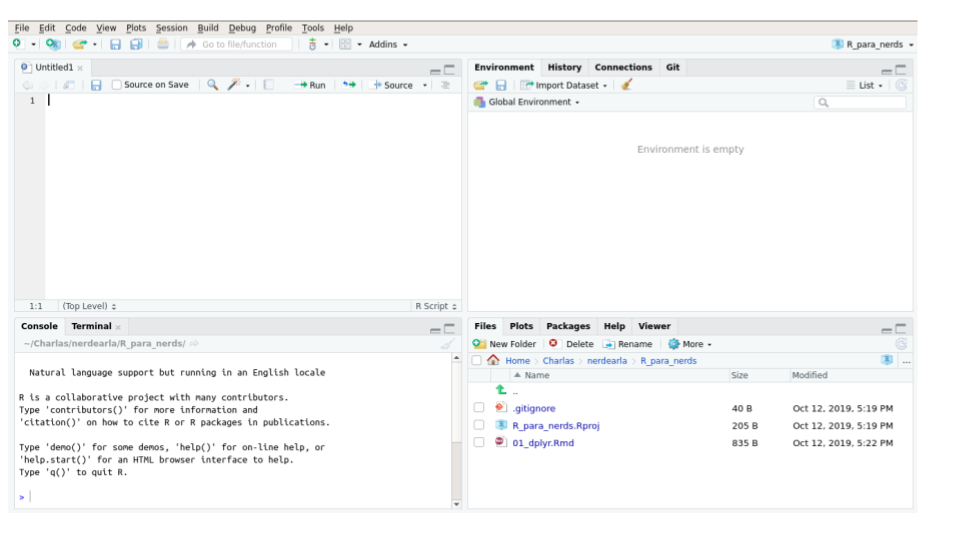
\includegraphics{img/rstudio.png}
\caption{Ventana de RStudio}
\end{figure}

Los dos paneles de la izquierda son las dos formas principales de interactuar con R.
El panel de abajo a la izquierda es \textbf{la consola}.
Es el lugar que te permite \emph{conversar} con R.
Podés escribir comandos que se van a ejecutar inmediátamente cuando aprietes Enter y cuyo resultado se va a mostrar en la consola.

Por ejemplo, hacé click en la consola, escribí \texttt{2\ +\ 2} y apretá Enter.
Vas a ver algo como esto:

\begin{Shaded}
\begin{Highlighting}[]
\DecValTok{2} \SpecialCharTok{+} \DecValTok{2}
\end{Highlighting}
\end{Shaded}

\begin{verbatim}
## [1] 4
\end{verbatim}

Le dijiste a R que sume 2 y 2 y R te devolvió el resultado: 4 (no te preocupes del \texttt{{[}1{]}} por ahora).
Eso está bueno si querés hacer una cuenta rápida o chequear algo pequeño, pero no sirve para hacer un análisis complejo y reproducible.

En el panel de arriba a la izquierda tenemos esencialmente un editor de texto.
Ahí es donde vas a escribir si querés guardar instrucciones para ejecutarlas en otro momento y donde vas a estar el 87\% de tu tiempo usando R.

A la derecha hay paneles más bien informativos y que tienen varias solapas que vamos a ir descubriendo a su tiempo.
Para destacar, arriba a la derecha está el ``environment'', que es forma de ver qué es lo que está ``pensando'' R en este momento.
Ahí vas a poder ver un listado de los datos que están abiertos y otros objetos que están cargados en la memoria de R.
Ahora está vacío porque todavía no cargaste ni creaste ningún dato.
Abajo a la derecha tienen un explorador de archivos rudimentario y también el panel de ayuda, que es donde vas a pasar el otro 13\% del tiempo usando R.

Entonces, para resumir:

\begin{figure}
\centering
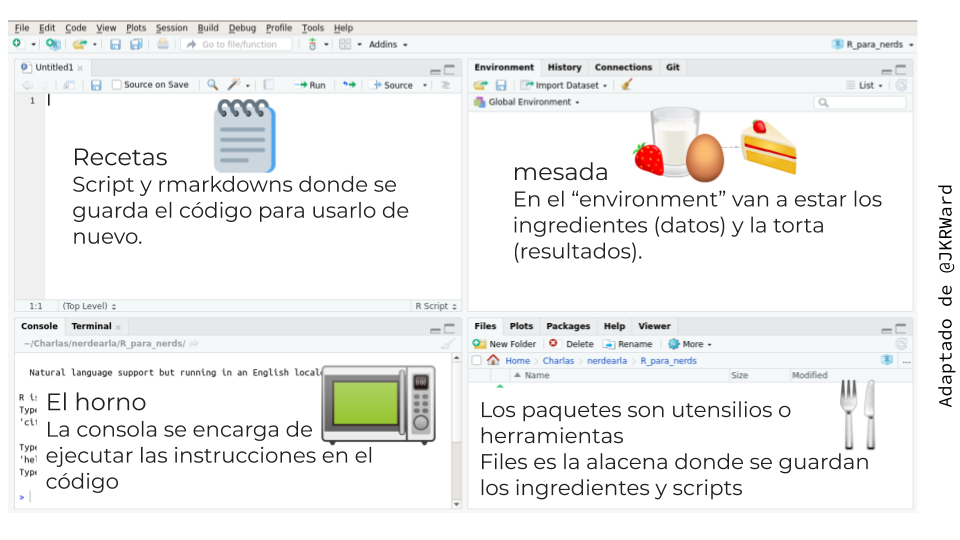
\includegraphics{img/rstudio-cocina.png}
\caption{La cocina de RStudio}
\end{figure}

\hypertarget{hablando-con-r}{%
\subsection{Hablando con R}\label{hablando-con-r}}

Ya viste cómo usar R como una calculadora.

\begin{Shaded}
\begin{Highlighting}[]
\DecValTok{2} \SpecialCharTok{+} \DecValTok{2}
\end{Highlighting}
\end{Shaded}

\begin{verbatim}
## [1] 4
\end{verbatim}

Si usaste fórmulas en Excel, esto es muy parecido a poner \texttt{=2+2} en una celda.
R entiende un montón de operaciones aritméticas escritas como seguramente ya te imaginás:

\begin{itemize}
\tightlist
\item
  \texttt{+}: sumar
\item
  \texttt{-}: restar
\item
  \texttt{*}: multiplicar
\item
  \texttt{/}: dividir
\item
  \texttt{\^{}}: exponenciar
\end{itemize}

Pero además conoce muchas otras operaciones.
Para decirle a R que calcule el seno de 1 hay que escribir esto:

\begin{Shaded}
\begin{Highlighting}[]
\FunctionTok{sin}\NormalTok{(}\DecValTok{1}\NormalTok{)}
\end{Highlighting}
\end{Shaded}

\begin{verbatim}
## [1] 0.841471
\end{verbatim}

Esto es similar a poner \texttt{=SIN(1)} en Excel.
La sintaxis básica para aplicar cualquier función es \texttt{nombre\_funcion(argumentos)}.

\textbf{Nota}: En Excel el nombre de las funciones dependen del idioma en el que está instalado.
Si lo usás en español, la función seno es \texttt{SEN()}.
En R, las funciones siempre se escriben igual (que coincide con el inglés).

\textbf{Desafío}

Decile a R que compute las siguientes operaciones:

\begin{itemize}
\tightlist
\item
  2 multiplicado por 2
\item
  3 al cuadrado
\item
  dos tercios
\item
  5 por 8 más 1
\end{itemize}

Al hacer todas estas operaciones, lo único que hiciste fue decirle a R que haga esos cálculos.
R te devuelve el resultado, pero no lo guarda en ningún lado.
Para decirle que guarde el resultado de una operación hay que decirle con qué ``nombre'' querés guardarlo.
El siguiente código hace eso:

\begin{Shaded}
\begin{Highlighting}[]
\NormalTok{x }\OtherTok{\textless{}{-}} \DecValTok{2} \SpecialCharTok{+} \DecValTok{2}
\end{Highlighting}
\end{Shaded}

La ``flechita'' \texttt{\textless{}-} es el operador de asignación, que le dice a R que tome el resultado de la derecha y lo guarde en una variable con el nombre que está a la izquierda.
Vas a ver que no te devele el resultado.
Para verlo, ejecutamos

\begin{Shaded}
\begin{Highlighting}[]
\NormalTok{x}
\end{Highlighting}
\end{Shaded}

\begin{verbatim}
## [1] 4
\end{verbatim}

Esto le dice a R que te ``imprima'' el contenido de la variable x.

\textbf{Desafío}

¿Qué te imaginás que va a pasar cuando ahora corra el siguiente código?

\begin{Shaded}
\begin{Highlighting}[]
\NormalTok{x }\SpecialCharTok{+} \DecValTok{2}
\end{Highlighting}
\end{Shaded}

Ponerle nombre a las variables es a veces la parte más difícil de escribir código.
A R le viene bien cualquier nombre de variable siempre y cuando no empiece con un número o un ``\_''.
Pero a los seres humanos que lean el código y tengan que interpretarlos les va a resultas más fácil entender qué hace la variable \texttt{promedio\_noches\_estadia} que la variable \texttt{xxy1}.

El consejo es tratar en lo posible usar nombre descriptivos y consistentes.
Por ejemplo, siempre usar minúsculas y separar palabras con ``\_''.

\textbf{Tip}: Para hacerse la vida más fácil existen ``guías de estilo'' para programar que explicitan reglas específicas para escribir código.
Por ejemplo \href{https://rpubs.com/FvD/guia-estilo-r}{esta} o \href{https://github.com/eliocamp/tesis/blob/master/docs/gu\%C3\%ADa_de_estilo.md}{esta otra}.
Se trata de reglas únicamente para los ojos humanos, y que no afectan en absoluto la eficiencia o correctitud de la programación.
En general, no existen guías buenas o malas, la idea es elegir una y ser consistente.
De esta manera, vas a poder entender tu código con más facilidad.

\hypertarget{extendiendo-r}{%
\subsection{Extendiendo R}\label{extendiendo-r}}

R es un lenguaje creado por personas que practican la estadística y pensado para la estadística, por lo que ya viene con un montón de métodos estadísticos incorporados, como \texttt{mean()} o \texttt{median()}.
Pero hay tantos métodos estadísticos como gente haciendo estadística así que es imposible que estén todos.
La solución es que podés ``agregarle'' a R funciones que no vienen instaladas por defecto pero que escribieron otras personas en forma de ``paquetes''.
¡Este es el poder de \textbf{la comunidad de R}!

Para instalar paquetes de R, la forma mas fácil es con la función \texttt{install.packages()}.
Entonces, por ejemplo,

\begin{Shaded}
\begin{Highlighting}[]
\FunctionTok{install.packages}\NormalTok{(}\StringTok{"readr"}\NormalTok{)}
\end{Highlighting}
\end{Shaded}

te instala un paquete que contiene funciones para leer datos.
Luego, usando el comando

\begin{Shaded}
\begin{Highlighting}[]
\FunctionTok{library}\NormalTok{(readr)}
\end{Highlighting}
\end{Shaded}

le decís a R que cargue las funciones que vienen en el paquete readr para usarlas.

\textbf{Desafío}: Instalá el paquete \{readr\} con el comando \texttt{install.packages("readr")\ en\ la\ consola.}

\textbf{Nota}: Si cerrás y volveś a abrir R, vas a tener que usar \texttt{library(readr)} nuevamente para acceder a la funcionalidad del paquete readr.
Sólo hace falta correr \texttt{install.packages("readr")} una vez por máquina.

\hypertarget{buscando-ayuda}{%
\subsection{Buscando ayuda}\label{buscando-ayuda}}

Entre la enorme cantidad de funciones que tiene R por defecto y las que se pueden agregar instalando paquetes externos, es imposible recordar todas las funciones y cómo usarlas.
Por eso, una gran proporción del tiempo que uses R vas a pasarlo leyendo documentación de funciones, ya sea para aprender a usarlas o porque no te acordás algún detalle.

Para acceder a la ayuda de una función usamos el signo de pregunta:

\begin{Shaded}
\begin{Highlighting}[]
\NormalTok{?sin}
\end{Highlighting}
\end{Shaded}

\textbf{Nota}: Otra forma de acceder a la ayuda de una función es poniendo el cursor sobre ella y apretando F1

Esto va a abrir el documento de ayuda para la función \texttt{sin()} que, como verás, tiene la documentación de las funciones trigonométricas que trae R por defecto.
Todas las ayudas de R vienen divididas en secciones:

\begin{description}
\item[Description]
Una descripción breve de la función o funciones que se documentan.
\item[Usage]
Nombre de los argumentos de la función.
La mayoría de las funciones trigonométricas tienen un solo argumento, que se llama \texttt{x}.
La función \texttt{atan2()} tiene dos argumentos, llamados \texttt{x} e \texttt{y}.
\item[Arguments]
Una descripción de cada argumento.
En este caso \texttt{x} e \texttt{y} son vectores numéricos o complejos.
Aunque todavía no sepas qué es un ``vector'', de esta descripción ya podés intuir que las funciones trigonométricas aceptan números complejos.
\item[Details]
Una descripción detallada de las funciones.
Por ejemplo, detalla qué es lo que devuelve la función \texttt{atan2()}, describe las unidades en las que tienen que estar \texttt{x} e \texttt{y}, etc..
\item[Value]
Describe qué tipo de valor devuelve la función.
\item[Examples]
(abajo de todo) Es la sección más importante y probablemente la que vas a buscar primero cuando te encuentres con una función nueva que no sabés cómo usar.
Acá vas a encontrar código de R de que ejemplifica el uso típico de la función.
Podes copiar y pegar el código en la consola y ver el resultado para entender como funciona.
\item[(Otras secciones)]
Pueden haber otras secciones que detallen distintas particularidades de la función, o referencias a los métodos implementados.
\end{description}

\textbf{Desafío}

Abrí y leé la ayuda de la función \texttt{sd()}.
Puede que haya cosas que aún no entiendas, pero tratá de captar la idea general.
¿Qué hace esa función?
¿Qué argumentos acepta?

\hypertarget{trabajar-con-proyectos-en-rstudio}{%
\chapter{Trabajar con proyectos en RStudio}\label{trabajar-con-proyectos-en-rstudio}}

Trabajar con proyectos de RStudio no solo hace tus análisis más ordenados y reproducibles, también hacen tu vida más simple.

Al comienzo posiblemente tengas un script y uno o dos archivos con datos, pero es posible que rápidamente te encuentres con una docena de archivos con nombres parecidos pero que pertenecen a análisis totalmente distintos.
Antes de que la cosa comience a complicarse te proponemos trabajar con proyectos.

\hypertarget{quuxe9-ventajas-tiene}{%
\subsection{¿Qué ventajas tiene?}\label{quuxe9-ventajas-tiene}}

\begin{itemize}
\tightlist
\item
  Te permite ``cuidar'' los datos que usas al ordenarnos en carpetas que diferencien entre la versión original o cruda y los datos limpios o los resultados finales.
\item
  Te permite compartir tu trabajo fácilmente con otras personas. Solo tendrías que compartir la carpeta del proyecto sabiendo que incluye todo lo necesario para que cualquiera reproduzca tu análisis.
\item
  Te permite publicar de manera ordenada tu código si vas a presentar o publicar tu trabajo.
\item
  Te permite continuar con lo que estabas haciendo hace una semana o hace un mes como si el tiempo no hubiera pasado. De alguna manera es un regalo para tu yo futuro.
\end{itemize}

\textbf{Primer desafío: Crea un nuevo proyecto en RStudio}

\begin{enumerate}
\def\labelenumi{\arabic{enumi}.}
\tightlist
\item
  Hacé click en el menú ``Archivo'' (``File'') y luego en ``Nuevo Proyecto'' (``New Project'').
\item
  Hacé click en ``Nueva Carpeta'' (``New Directory'').
\item
  Hacé click en ``Nuevo Proyecto'' (``New Project'').
\item
  Escribí el nombre de la carpeta que alojará a tu proyecto, por ejemplo ``mi\_proyecto''
\item
  Si aparece (y sabés usarlo), seleccioná ``Crear un repositorio de git'' (``Create a git repository'').
\item
  Hacé click en ``Crear Proyecto'' (``Create Project'').
\end{enumerate}

Si todo salió bien, ahora deberías tener una nueva carpeta que se llama \emph{mi\_proyecto}.
Pero si bien es una carpeta común y corriente, le llamamos proyecto porque además contiene un archivo con el mismo nombre \emph{mi\_proyecto.Rproj} (o solo \emph{mi\_proyecto} si en tu computadora no ves la extensión de los archivos).

\hypertarget{abrir-un-proyecto}{%
\subsection{Abrir un proyecto}\label{abrir-un-proyecto}}

La manera más simple de abrir un proyecto es abriendo la carpeta que lo contiene y haciendo doble click sobre el archivo \emph{mi\_proyecto.Rproj}.
Al hacer esto se abrirá RStudio y la sesión de R en la misma carpeta y, por defecto, cualquier archivo que quieras abrir o guardar lo hará en esa misma ubicación.
Esto ayuda a mantener tu trabajo ordenado y que luego sea simple retomar o compartir lo que hiciste.

RStudio permite tener varios proyectos abiertos, y esto es posible porque justamente cada proyecto tiene su propia carpeta.
Si en algún momento trabajas con proyectos en paralelo vas a poder hacerlo sin que el código o los resultados de un análisis interfieran con otro.

\textbf{Segundo desafío: Abrí tu nuevo proyecto desde el explorador de archivos}

\begin{enumerate}
\def\labelenumi{\arabic{enumi}.}
\tightlist
\item
  Cerrá RStudio
\item
  Desde el explorador de archivos, buscá la carpeta donde creaste tu proyecto.
\item
  Hacé doble click en el archivo que tiene el nombre de tu proyecto (y que termina con \emph{.Rproj}) que encontrarás en esa carpeta.
\end{enumerate}

\hypertarget{cuxf3mo-se-organiza}{%
\subsection{¿Cómo se organiza?}\label{cuxf3mo-se-organiza}}

No existe una ``mejor'' forma de organizar un proyecto pero acá van algunos principios generales que nos hacen la vida más simple::

\begin{itemize}
\tightlist
\item
  \textbf{Tratar los datos como sólo de lectura} Es posible que la toma de los datos que querés analizar te haya costado mucho trabajo, o te haya costado conseguirlos. Trabajar con datos de forma interactiva (por ejemplo, en Excel) tiene la ventaja de permitirte hacer algunos análisis rápidamente pero al mismo tiempo tiene la desventaja de que esos datos pueden ser modificados fácilmente. Esto significa que a veces no conozcas de la procedencia de los datos, o no recuerdes cómo los modificaste desde que los obtuviste. Por lo tanto, es una buena idea tratar los datos como ``sólo de lectura'' y nunca modificar los archivos originales.
\item
  \textbf{Limpieza de datos} En muchos casos tus datos estarán ``sucios'', necesitarán un preprocesamiento importante para organizarlos en un formato que R (o cualquier otro lenguaje de programación) pueda analizados fácilmente. Esta tarea se denomina a veces ``amasado'' o ``masticado de datos''. Es una buena costumbre guardar el código que te permitió limpiar estos datos por si los volvieras a necesitar. También es recomendable guardar esa versión de los datos limpios, de ``sólo lectura'', para que puedas usarlos en tu análisis sin necesidad de repetir cada vez todo el proceso de limpieza de los datos.
\item
  \textbf{Tratar las salidas o resultados generados como descartables} Cualquier resultado (gráficos, tablas, valores) debe poder repetirse o rehacerse a partir del código guardado. Si bien las pruebas rápidas para \emph{ver si el código funciona} se pueden hacer en la consola, es importante guardar el código que genera los resultados y asegurarnos de que sean reproducibles. Aún mejor, si organizas esos resultados en distintas sub-carpetas, luego tendrás todo aún más ordenado.
\end{itemize}

\hypertarget{ordenando-auxfan-muxe1s}{%
\subsection{Ordenando aún más}\label{ordenando-auxfan-muxe1s}}

Si tenés alguna experiencia programando con R es posible que tengas estás lineas al comienzo de alguno de tus scripts o si nunca las usaste, seguro viste que alguien más lo hacia:

\begin{Shaded}
\begin{Highlighting}[]
\FunctionTok{setwd}\NormalTok{(}\StringTok{"/Users/pao/una\_carpeta/al/proyecto\_importante"}\NormalTok{)}
\FunctionTok{rm}\NormalTok{(}\AttributeTok{list =} \FunctionTok{ls}\NormalTok{())}
\end{Highlighting}
\end{Shaded}

La primera línea \emph{setea} o le avisa a R cual será la carpeta donde va a trabajar. \emph{Con el uso de proyectos esto está prácticamente solucionado} porque al abrir el proyecto ya sea desde el explorador de archivos haciendo doble click en el archivo con extensión \emph{Rproj} o desde RStudio, R sabrá que ese directorio será el de trabajo.

Pero también te dijimos que era una buena práctica organizar las diferentes partes del proyecto en subcarpetas, como por ejemplo colocar los datos en una subcarpeta llamada ``datos'', los informes en otra y tal vez las figuras en una subcarpeta distinta dentro del proyecto. ¿Cómo hacemos para que R lea un archivo que no está en la carpeta de trabajo? Podríamos escribir el camino hacia ese archivo, por ejemplo \texttt{"datos/mi\_archivo\_de\_datos.csv"} pero si queremos compartir el código a otra persona que tal vez tiene un sistema operativo distinto y usa la barra invertida \texttt{\textbackslash{}} va a estar en problemas al intentar correr esa línea.

Para solucionar estos problemas existe el paquete \texttt{\{here\}}, que funciona independientemente del sistema operativo. Su función principal \texttt{here()} recibe como argumentos el camino hacia el archivo que se quiere leer, siempre entre comillas y separados por comas, así:

\begin{Shaded}
\begin{Highlighting}[]
\NormalTok{mis\_datos }\OtherTok{\textless{}{-}} \FunctionTok{read\_csv}\NormalTok{(}\FunctionTok{here}\NormalTok{(}\StringTok{"datos"}\NormalTok{, }\StringTok{"mi\_archivo\_de\_datos.csv"}\NormalTok{))}
\end{Highlighting}
\end{Shaded}

Internamente este paquete puede identificar cual es el directorio de trabajo (por ejemplo detectando que hay un archivo \emph{.Rproj}) y busca a partir de ahí la subcarpeta ``datos'' y adentro de ella el archivo ``mi\_archivo\_de\_datos.csv''.

La segunda línea del código inicial se usa para borrar los elementos que creamos en el análisis normalmente cuando cambiamos de tema o empezamos a trabajar con algo distinto. Esto está bien porque no queremos arrastrar análisis que hicimos en un proyecto a otro, necesitamos que sean autocontenidos y \emph{reproducibles}. El problema es que este comando \textbf{no} borra los paquetes activados o las opciones usuario que hayamos seteado.

\hypertarget{borruxf3n-y-cuenta-nueva-todos-los-duxedas}{%
\subsection{Borrón y cuenta nueva\ldots{} todos los días!}\label{borruxf3n-y-cuenta-nueva-todos-los-duxedas}}

¿Cómo nos aseguramos de que el análisis sea realmente reproducible?
Esta es una pregunta bastante amplia y hay muchas herramientas para resolver este problema.
Por ahora nos vamos a concentrar en que al menos en tu computadora puedas repetir los cálculos o el análisis desde cero.
Y además de organizar proyectos y no modificar los datos originales, ¿cómo podés asegurarte de que guardaste todo el código que estuviste escribiendo y usaste?
La manera más directa es reiniciar la sesión de R y correr el código de nuevo, si da error o no devuelve lo que esperabas significa que te faltó guardar algún paso.

Tip: Podés reiniciar la sesión de R con el atajo \texttt{Ctrl+Shif+F10}

Esto puede pasar si por ejemplo leés una base de datos en memoria pero no guardás el código que lo hace.
Mientras estemos trabajando, R tendrá esa base de datos en memoria y podremos hacer cálculos y gráficos.
Por defecto además RStudio va a recordar las variables que estés usando mañana o pasado en un archivo oculto (.RData) a menos que le indiques lo contrario.
Y si bien suena práctico volver a R al otro día y tener el análisis tal cual lo dejamos, esto puede significar que nunca nos demos cuenta que nos faltó guardar una línea de código clave en nuestro análisis.

\textbf{Tercer desafío: Configurá RStudio}

\begin{enumerate}
\def\labelenumi{\arabic{enumi}.}
\tightlist
\item
  Hacé click en el menú ``Herramientas (''Tools'') y luego ``Opciones globales'' (``Global Options'').
\item
  Destildá la opción ``Recuperar .RData al inicio de la sesión'' (``Restore .RData into workspace at startup'').
\item
  Hacé click en ``Aplicar'' (``Apply'').
\end{enumerate}

\hypertarget{introducciuxf3n-a-rmarkdown}{%
\chapter{Introducción a RMarkdown}\label{introducciuxf3n-a-rmarkdown}}

Es posible que en tu trabajo tengas que presentar informes o resultados de tu análisis de datos.
Tal vez te hayas encontrando guardando una y otra vez gráficos y tablas o copiando resultados de un archivo al otro hasta que el informe quedó como querías.
Los archivos y el paquete \textbf{RMarkdown} vienen al rescate.

Un archivo de R Markdown (generalmente con la extensión \texttt{.Rmd}), a diferencia de un script \texttt{.R}, es un archivo de texto plano que combina código de R que genera resultados (gráficos, tablas, etc\ldots) y el texto que lo describe.
Al poder intercalar cálculos y gráficos con su análisis o explicación, se unifica el flujo de trabajo y deja de ser necesario guardar figuras o tablas para luego insertarlas en un documento de texto.
Esto es muy importante si buscamos que nuestro trabajo sea reproducible, pero además ahorra tiempo.

\hypertarget{creando-archivos-.rmd}{%
\section{Creando archivos .Rmd}\label{creando-archivos-.rmd}}

En RStudio podés crear un nuevo archivo de R Markdown con el menú desplegable:

File → New File → R Markdown

Y se abrirá un menú donde podés agregar el título de tu informe y tu nombre.
Por ahora vamos a usar el formato HTML como salida, pero más adelante vas a ver que hay muchos otros formatos de salida posibles.

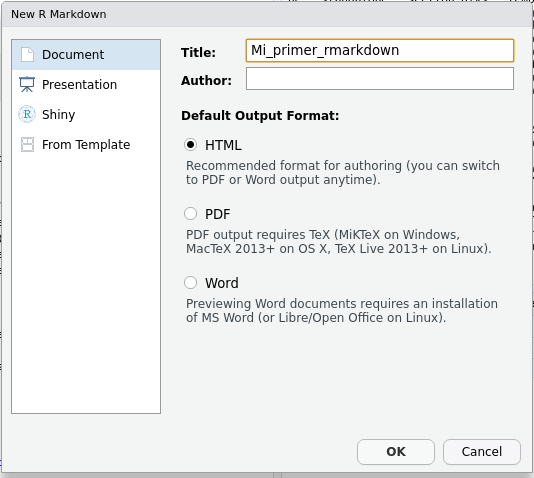
\includegraphics{img/nuevo-rmd.png}

Al aceptar, se abrirá un nuevo archivo con una plantilla de ejemplo (en inglés).

\textbf{Primer desafío: Creá un nuevo archivo R Markdown}

Revisá la plantilla que trae el documento.
¿Podés identificar los bloques de código?

Para generar el archivo de salida, el paquete \textbf{knitr} (que viene de \emph{tejer} en inglés) ejecutará el código en una sesión independiente de R e interpretará el texto, su formato y cualquier otra cosa que agreguemos (por ejemplo imágenes o links externos).
Esto significa que nuestro archivo debe tener \textbf{todo} lo necesario para generar el análisis y si nos olvidamos de algo va a dar error.

Por esta razón es recomendable \emph{knitear} el archivo seguido, para encontrarnos con los errores a tiempo y de paso asegurarnos que el análisis es reproducible.

\textbf{Segundo desafío: kniteá tu R Markdown}

Aprovechando la plantilla de RStudio, obtené el archivo de salida en formato HTML haciendo click en el botón \textbf{knit} (el que tiene un ovillo de lana y un par de agujas!).

\hypertarget{estructura-de-un-.rmd}{%
\section{Estructura de un .Rmd}\label{estructura-de-un-.rmd}}

Cualquier archivo de este tipo tiene 3 partes principales:

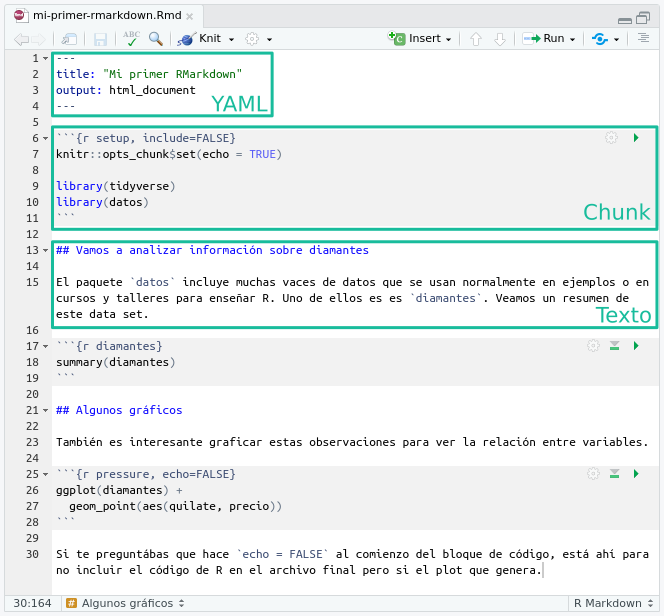
\includegraphics{img/rmd-ejemplo-secciones.png}

(Podés encontrar este archivo de ejemplo \href{files/mi-primer-rmarkdown.Rmd}{acá}.)

\hypertarget{encabezado}{%
\subsection{Encabezado}\label{encabezado}}

El encabezado es una serie de instrucciones organizadas entre tres guiones (\texttt{-\/-\/-}) que determinan las propiedades globales del documento, como el título, el formato de salida, información de autoría, etc\ldots{} También ahí se pueden cambiar opciones asociadas al formato de salida, como el estilo de la tabla de contenidos o índice.

Éstas propiedades se definen en un formato llamado \href{https://es.wikipedia.org/wiki/YAML}{YAML}, el cual permite definir listas jerarquizadas de una forma humanamente legible.
Por ejemplo:

\begin{Shaded}
\begin{Highlighting}[]
\PreprocessorTok{{-}{-}{-}}
\FunctionTok{title}\KeywordTok{:}\AttributeTok{ }\StringTok{"Mi primer RMarkdown"}
\FunctionTok{output}\KeywordTok{:}\AttributeTok{ }
\AttributeTok{  }\FunctionTok{html\_document}\KeywordTok{:}
\AttributeTok{    }\FunctionTok{code\_download}\KeywordTok{:}\AttributeTok{ }\CharTok{true}
\AttributeTok{    }\FunctionTok{toc}\KeywordTok{:}\AttributeTok{ }\CharTok{true}
\AttributeTok{    }\FunctionTok{toc\_float}\KeywordTok{:}\AttributeTok{ }\CharTok{false}
\PreprocessorTok{{-}{-}{-}}
\end{Highlighting}
\end{Shaded}

define dos variables principales, ``title'' y ``output''.
``Output'' a su vez contiene un elemento ``htm\_document'', el cual contiene tres elementos: ``code\_download'', ``toc'' y ``toc\_float''.

Es muy importante mantener el escalonado, o \emph{identación} de los elementos, ya que ésta define la jerarquía de cada elemento.
Muchos de los errores a la hora de knitear ocurren porque el archivo tiene problemas en la identación del encabezado.

\hypertarget{bloques-de-cuxf3digo}{%
\subsection{Bloques de código}\label{bloques-de-cuxf3digo}}

El código de R que va a leer datos, analizarlos y generar figuras, tablas o números se organiza en bloques (o \texttt{chunks}) delimitados por tres acentos graves (\texttt{\textasciigrave{}\textasciigrave{}\textasciigrave{}}) y se diferencia del resto de archivo con un fondo gris.
Todo lo que incluyas entre estos delimitadores será interpretado por R como código e intentará ejecutarlo al \emph{knitear} el archivo.
Cualquier resultado del código (gráficos, tablas, texto, etc\ldots) será insertado en el documento final en el mismo orden que están en el archivo R Markdown.

Para insertar un nuevo chunk podés:

\begin{itemize}
\tightlist
\item
  Usar el botón \textbf{Insert}
\item
  El atajo de teclado Ctrl+Alt+I
\item
  Escribir a mano!
\end{itemize}

El código en cada bloque se ejecuta como si fuera ejecutado en la terminal y todo resultado se muestra en el documento (ya vamos a ver formas de controlar esto).
Por ejemplo, este bloque de código

\begin{verbatim}
```{r sumar}
1 + 1
```
\end{verbatim}

va a insertar esto en el documento de salida:

\begin{verbatim}
[1] 2
\end{verbatim}

Es muy importante no romper los límites de los bloques.
Un problema común es accidentalmente eliminar un acento grave al final de un bloque de código y que luego el documento no knitee correctamente.
Si al knitear te sale un error como ``attempt to use zero-length variable name'', revisá bien que todos tus bloques de código estén correctamente definidos.

Los bloques pueden tener nombre, lo cual es útil para identificar donde ocurren los errores al momento de \emph{knitear} pero también para tener una pista de lo que hace el código que incluye.

Si bien el código se corre cuando uno knitea, cuando estés escribiendo un informe es muy cómodo ir corriendo bloques individuales interactivamente como si fuera en la consola.

Para correr una línea de código, tendrás que pararte sobre esa línea y apretar:

Ctrl+Enter

Pero también podés correr el código de todo el chunk con:

Ctrl+Shift+Enter

Los resultados van a aparecer inmediatamente debajo del bloque.

\textbf{Cuarto desafío: Sumá un chunk a tu archivo}

Usando el archivo con el que venís trabajando insertá un nuevo chunk y:

\begin{enumerate}
\def\labelenumi{\arabic{enumi}.}
\tightlist
\item
  Cargá el paquete readr.
\item
  Creá una variable que se llame \texttt{variable\_prueba} y asignale un valor.
\item
  Mostrá ese valor.
\item
  Volvé a \emph{knitear} el archivo para ver el resultado
\end{enumerate}

Finalmente, es posible que te encuentres mencionando resultados en el texto, por ejemplo algo así como ``el porcentaje de ocupación para el mes de enero fue del 95\%''.
Y también es posible que ese valor cambie si utilizas una base de datos distinta o si luego generas un informe pero para un mes siguiente.
Las chances de de que te olvides de actualizar ese ``95'' son super altas, por eso R Markdown también tiene la posibilidad de incorporar código en línea con el texto.

Si tenés una una variable \texttt{ocupacion} que vale ``95\%'':

\begin{Shaded}
\begin{Highlighting}[]
\NormalTok{ocupacion }\OtherTok{\textless{}{-}} \StringTok{"95\%"}
\end{Highlighting}
\end{Shaded}

Para mencionarla en el texto entonces escribirías:

\begin{quote}
El porcentaje de ocupación para el mes de enero fue del \texttt{\textasciigrave{}r\ ocupacion\textasciigrave{}}.
\end{quote}

y el resultado en el documento kniteado sería

\begin{quote}
El porcentaje de ocupación para el mes de enero fue del 95\%.
\end{quote}

prueba: \texttt{95\%}

\hypertarget{el-texto-propio-del-documento.}{%
\subsection{El texto propio del documento.}\label{el-texto-propio-del-documento.}}

Este es el texto dirigido a las personas que van a leer el reporte.
Incluirá una introducción, descripción de los datos y de los resultados; es lo que escribirías en el archivo de Word.

A diferencia de Word, el formato del texto se define usando \protect\hyperlink{markdown}{markdown}(\url{https://es.wikipedia.org/wiki/Markdown}{]}, que es un lenguaje simple que permite indicar si un texto va en negrita, cursiva, es un título, etc\ldots usando símbolos especiales dentro del texto.

\hypertarget{markdown}{%
\section{Markdown}\label{markdown}}

Markdown permite escribir en texto plano pero definiendo el formato usando símbolos.
Por ejemplo podés resaltar con \textbf{negrita} usando dos asteriscos así: \texttt{**negrita**} o \emph{italizada} con un asterisco de cada lado: \texttt{*itálicas*}.

También podés hacer una lista de elementos utilizando asteriscos:

\begin{verbatim}
* la negrita se consigue con dos asteriscos
* la italizada con un asterisco
* y para resaltar código se usa el acento grave `
\end{verbatim}

o guiones medios:

\begin{verbatim}
- la negrita se consigue con dos asteriscos
- la italizada con un asterisco
- y para resaltar código se usa el acento grave `
\end{verbatim}

Ambas listas se van a ver de esta manera:

\begin{itemize}
\tightlist
\item
  la negrita se consigue con dos asteriscos
\item
  la italizada con un asterisco
\item
  y para resaltar código se usa el acento grave `
\end{itemize}

Si en realidad querés una lista numerada, simplemente comenzá el renglón un número y un punto.
Podrías usar siempre el mismo número, markdown se encarga del resto:

\begin{verbatim}
1. la negrita se consigue con dos asteriscos
1. la italizada con un asterisco
1. y para resaltar código se usa el acento grave `
\end{verbatim}

Ahora la lista numerada se ve así:

\begin{enumerate}
\def\labelenumi{\arabic{enumi}.}
\tightlist
\item
  la negrita se consigue con dos asteriscos
\item
  la italizada con un asterisco
\item
  y para resaltar código se usa el acento grave `
\end{enumerate}

Podés agregar títulos con distinta jerarquía agregando \texttt{\#} al comienzo.
Esto además define secciones dentro del documento:

\begin{verbatim}
# Título
## El primer subtítulo
### Otro subtítulo de menor jerarquía
#### Otro más, y podría seguir!
\end{verbatim}

Podés escribir estos símbolos a mano o usando el Editor Visual de RStudio (sólo disponible para la versión 1.4 en adelante) haciendo click en el ícono de compás que está a la derecha del documento (
\includegraphics{img/icono-editor-visual.png}) .
El Editor Visual permite dar formato al texto usando markdown sin saber usar markdown.

\textbf{Tercer desafío: Agregale texto a tu archivo}

Borrá el contenido del archivo \texttt{.Rmd} que creaste (pero no el encabezado!) y probá escribir algo y darle formato.
Luego volvé a apretar el botón \textbf{knit} para ver el resultado.

Markdown permite muchas otras cosas, por ejemplo:

Podés agregar un link a una página externa: \texttt{{[}texto\ que\ se\ muestra\ con\ el\ link{]}(http://google.com)}.
Resultado: \href{http://google.com}{texto que se muestra con el link}

Podés incluir una imagen: \texttt{!{[}descripción\ de\ la\ figura{]}(https://placekitten.com/200/100)}: Resultado:

\begin{figure}
\centering
\includegraphics{https://placekitten.com/200/100}
\caption{descripción de la figura}
\end{figure}

Y también podés agregar ecuaciones (usando \href{https://es.wikipedia.org/wiki/LaTeX}{LaTeX}) en la misma línea (esto:\texttt{\$E\ =\ mc\^{}2\$} se ve así: \(E = mc^2\)) o en una línea propia.
Esto:

\begin{verbatim}
$$
y = \mu + \sum_{i=1}^p \beta_i x_i + \epsilon
$$
\end{verbatim}

se ve así:

\[
y = \mu + \sum_{i=1}^p \beta_i x_i + \epsilon
\]

Podés revisar la guía rápida de Markdown desde RStudio (en inglés):

Help → Markdown Quick Reference

\hypertarget{lectura-de-datos-ordenados}{%
\chapter{Lectura de datos ordenados}\label{lectura-de-datos-ordenados}}

\hypertarget{descargando-datos}{%
\section{Descargando datos}\label{descargando-datos}}

Antes de poder leer cualquier dato en R, primero hay que encontrarlo y descargarlo.
El Ministerio de Turismo mantiene un portal de datos abierto llamado \href{http://datos.yvera.gob.ar/}{Yvera} donde podés buscar y descargar datos relacionados con el turismo en Argentina.

En esta sección vamos a descargar una serie de tiempo a partir de la Encuesta de Viajes y Turismo de los Hogares (EVyTH).

Primero, ingresá a \url{http://datos.yvera.gob.ar/}, donde te vas a encontrar con la páigna principal de Yvera.



\begin{center}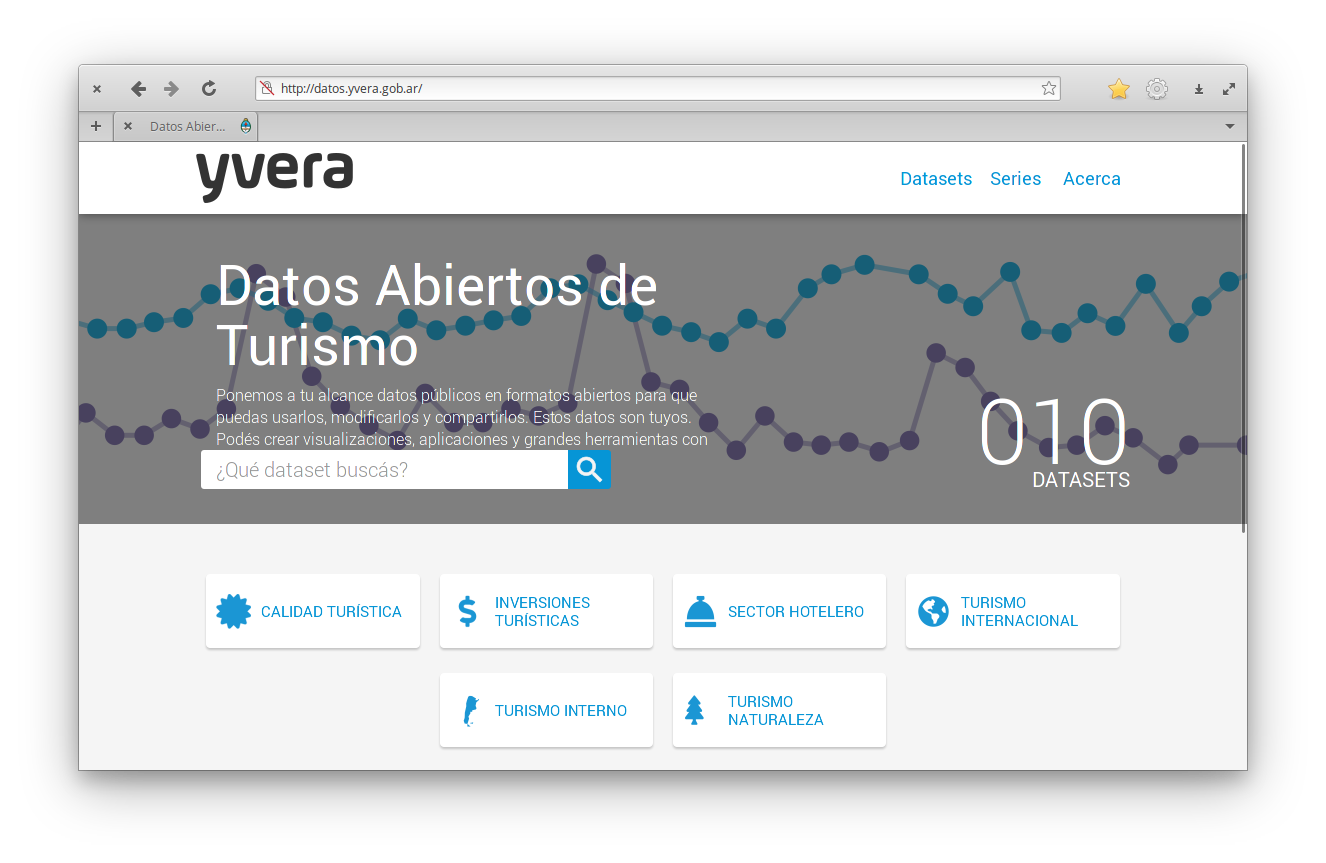
\includegraphics[width=1\linewidth]{img/yvera-principal} \end{center}

La base de datos que vamos a descargar está en el área de Turismo Interno así que hacé click en \href{http://datos.yvera.gob.ar/dataset?groups=turismo-interno}{ese ícono} para navegar a la sección de datasets correspondiente.



\begin{center}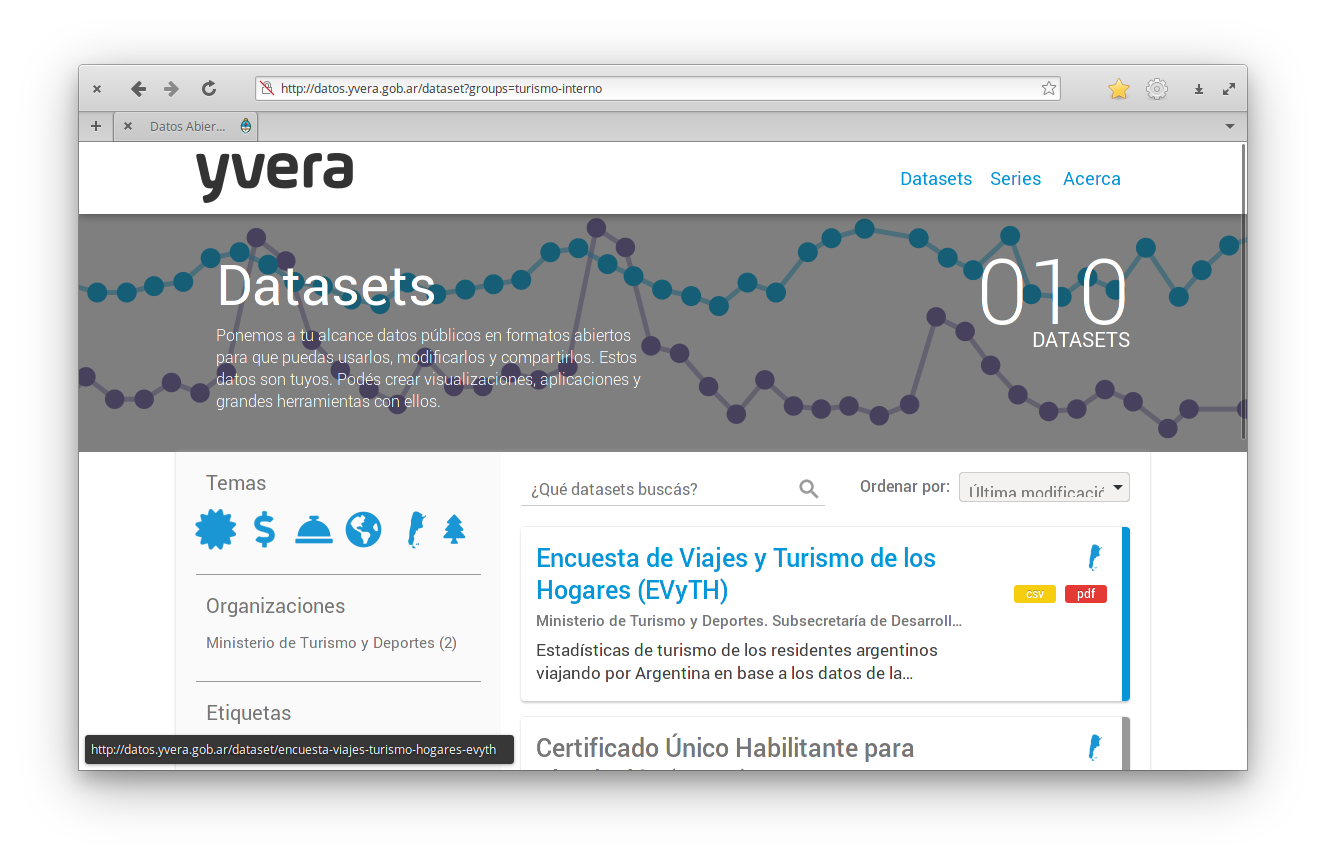
\includegraphics[width=1\linewidth]{img/yvera-interno} \end{center}

Al momento que escribimos esta guía el primer set de datos que aparece es la Encuesta de Viajes y Turismo de los Hogares (EVyTH). Hacé click ahí para ir a \href{http://datos.yvera.gob.ar/dataset/encuesta-viajes-turismo-hogares-evyth}{la página de este set de datos}.



\begin{center}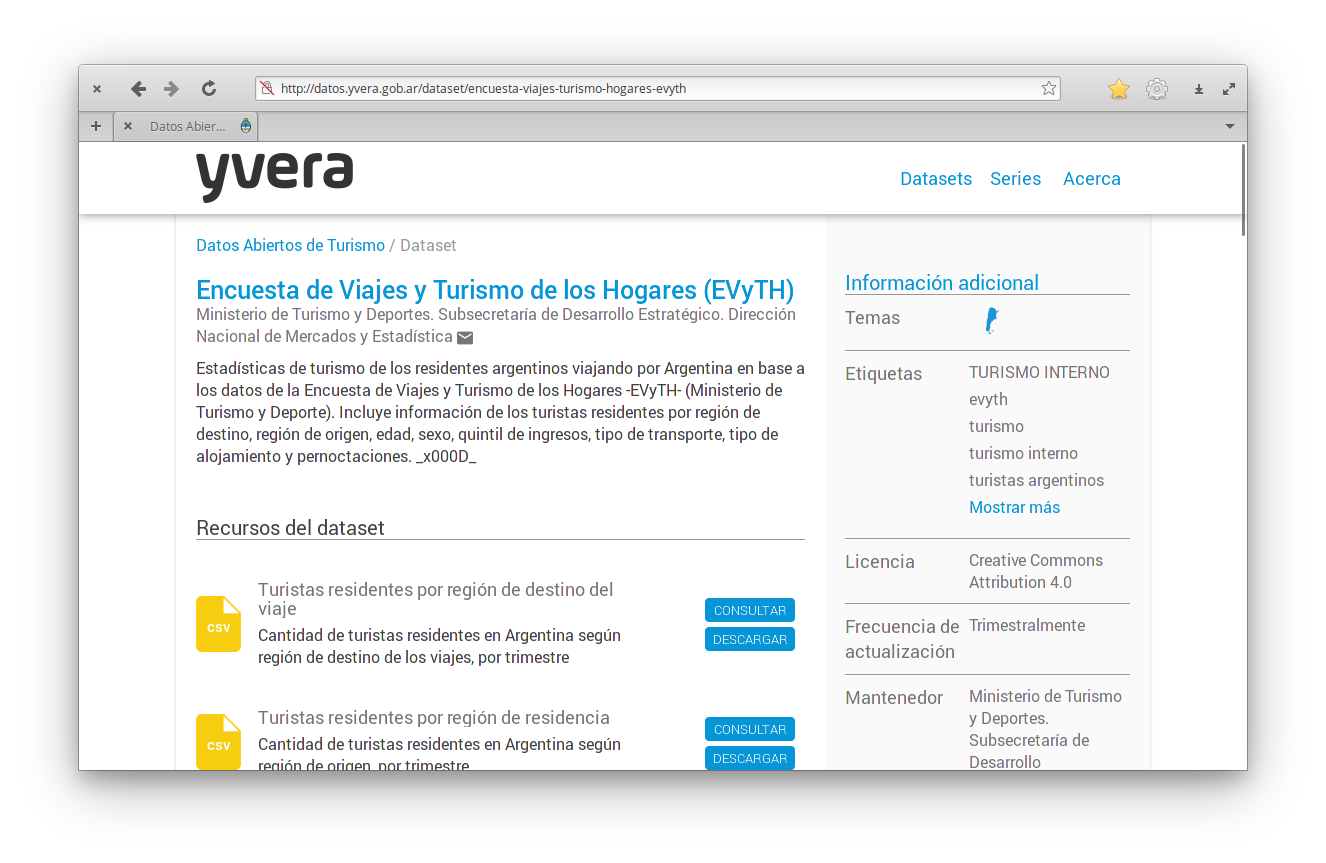
\includegraphics[width=1\linewidth]{img/yvera-evyth} \end{center}

Este set de datos tiene distintos recursos.
Varios son datos, como ``Turistas residentes por región de destino del viaje'' o ``Turistas residentes por edad'', pero también hay un recurso llamado ``Ficha Técnica: EVyTH''.
Este es \href{http://datos.yvera.gob.ar/dataset/945e10f1-eee7-48a2-b0ef-8aff11df8814/resource/f41af122-ca31-4654-907b-a9cd57b80651/download/2021.01.05_evyth.pdf}{un PDF} con la descripción de los datos así como consideraciones metodológicas relevantes.
Es importante que si vas a usar datos siempre mires la ficha técnica para hacerte una idea de las limitaciones metodológicas que pueden tener estos datos.

Por ahora vamos a descargar la \href{http://datos.yvera.gob.ar/dataset/encuesta-viajes-turismo-hogares-evyth/archivo/abdacfcd-4a6c-4283-9abb-c1352def52e1}{serie de Turistas residentes por edad}.



\begin{center}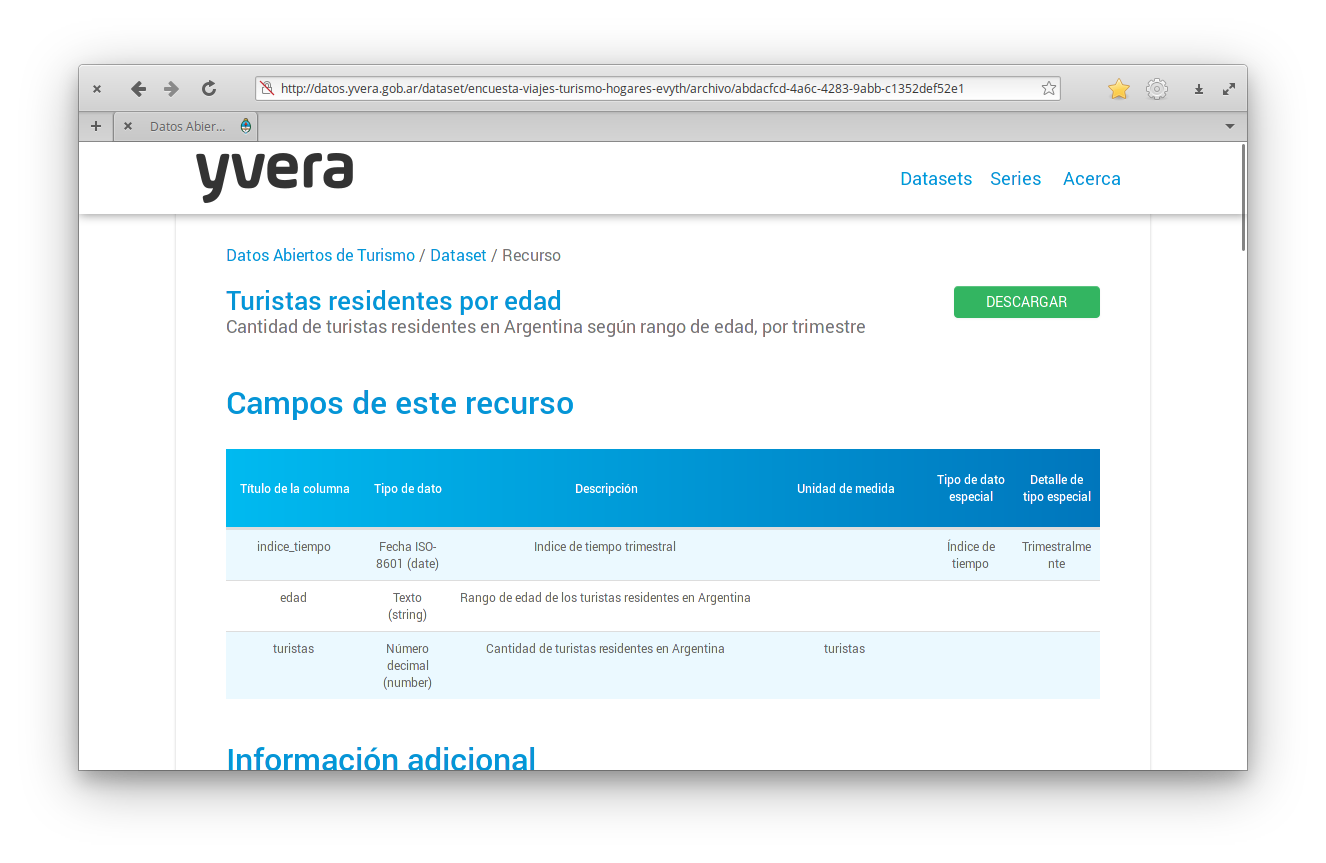
\includegraphics[width=1\linewidth]{img/yvera-evyth-edad} \end{center}

En esta pantalla te vas a encontrar con una descripción del set de datos y sus variables.
Para descargar los datos hay que hacer click en el botón que dice ``\href{http://datos.yvera.gob.ar/dataset/945e10f1-eee7-48a2-b0ef-8aff11df8814/resource/abdacfcd-4a6c-4283-9abb-c1352def52e1/download/tur_int_turistas_residentes_edad_serie.csv}{DESCARGAR}''.
Guardalo en una carpeta dentro del proyecto (recomedamos organizar los datos en una carpeta llamada ``datos'') y ya está listo para leer.

Pero si tuvieras que realizar un informe mensual sobre estos datos tendrías que hacer toda esta descarga manual cada vez que se actualiza el informe.
La gracia de usar código es automatizar todo lo más posible, así que en vez de descargar manualmente el archivo, se puede descargar automáticamente desde el código de R.

Para eso, primero necesitás la dirección (URL) del set de datos.
Eso se consigue yendo a \href{http://datos.yvera.gob.ar/dataset/encuesta-viajes-turismo-hogares-evyth/archivo/abdacfcd-4a6c-4283-9abb-c1352def52e1}{la página del set de datos} y en vez de hacer click en DESCAGAR, haciendo

Click derecho → Copiar dirección del enlace

La URL de la esta serie es \texttt{http://datos.yvera.gob.ar/dataset/945e10f1-eee7-48a2-b0ef-8aff11df8814/resource/abdacfcd-4a6c-4283-9abb-c1352def52e1/download/tur\_int\_turistas\_residentes\_edad\_serie.csv}.
Guaramos eso en una variable en R

\begin{Shaded}
\begin{Highlighting}[]
\NormalTok{turistas\_edad\_url }\OtherTok{\textless{}{-}} \StringTok{"http://datos.yvera.gob.ar/dataset/945e10f1{-}eee7{-}48a2{-}b0ef{-}8aff11df8814/resource/abdacfcd{-}4a6c{-}4283{-}9abb{-}c1352def52e1/download/tur\_int\_turistas\_residentes\_edad\_serie.csv"}
\end{Highlighting}
\end{Shaded}

Y también definimos la ruta donde descargar el archivo

\begin{Shaded}
\begin{Highlighting}[]
\NormalTok{turistas\_edad\_archivo }\OtherTok{\textless{}{-}} \StringTok{"datos/turistas\_edad.csv"}
\end{Highlighting}
\end{Shaded}

Y finalmente usamos la función \texttt{download.file()} para descargar el archivo.

\begin{Shaded}
\begin{Highlighting}[]
\FunctionTok{download.file}\NormalTok{(}\AttributeTok{url =}\NormalTok{ turistas\_edad\_url, }\AttributeTok{destfile =}\NormalTok{ turistas\_edad\_archivo)  }
\end{Highlighting}
\end{Shaded}

Y esto va a descargar la última versión de los datos.

\hypertarget{leer-datos-csv}{%
\section{Leer datos csv}\label{leer-datos-csv}}

Existen muchas funciones distintas para leer datos dependiendo del formato en el que están guardados.
Para datos tabulares, la forma más útil es el formato csv, que es un archivo de texto plano con datos separados por coma.

Para importar datos hace falta escribir el código correspondiente pero también podés aprovechar el entorno gráfico de RStudio:

File → Import Dataset → From Text (readr)\ldots{}

Esto te va abrir una ventana donde podrás elegir el archivo a importar (en este caso el archivo \texttt{turistas\_edad.csv} que está dentro de la capeta \texttt{datos} del proyecto) y otros detalles.

\begin{Shaded}
\begin{Highlighting}[]
\NormalTok{knitr}\SpecialCharTok{::}\FunctionTok{include\_graphics}\NormalTok{(}\StringTok{"img/importar{-}edad{-}xlsx.png"}\NormalTok{)}
\end{Highlighting}
\end{Shaded}

\begin{center}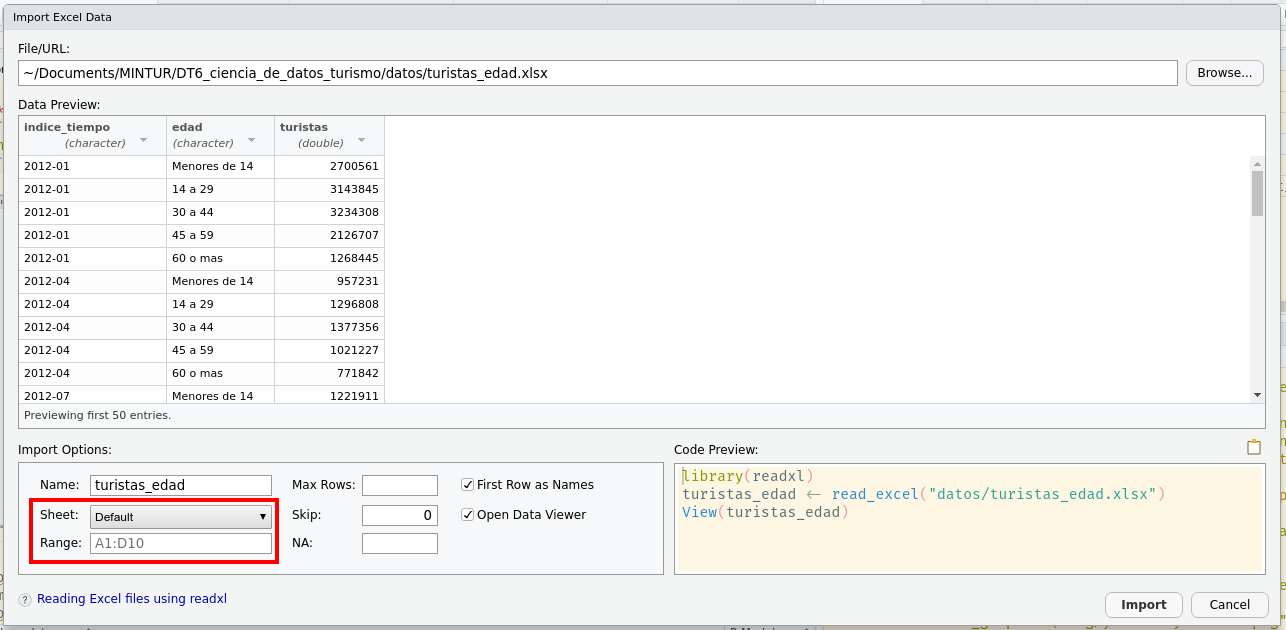
\includegraphics[width=1\linewidth]{img/importar-edad-xlsx} \end{center}

En la pantalla principal vas a poder previsualizar los datos y ver que pinta tienen.
Abajo a la izquierda tenés varias opciones: el nombre que vas a usar para la variable (en este caso llamaremos \texttt{turistas\_edad}), si la primera fila contiene los nombres de las columnas (\texttt{First\ Row\ as\ Names}), qué delimitador tienen los datos (en este caso \texttt{comma}, pero podría ser punto y coma u otro), etc\ldots{}

Y abajo a la derecha es el código que vas a necesitar para efectivamente importar los datos.
Podrías apretar el botón ``Import'' para leer los datos pero si bien es posible, al mismo tiempo esas líneas de código no se guardan en ningún lado y entonces nuestro trabajo luego no se puede reproducir.
Por eso, te proponemos que copies ese código, cierres esa ventana con el botón ``Cancel'', y pegues el código en el archivo donde estés trabajando.
Cuando lo ejecutes, se va a generar la variable \texttt{turistas\_edad} con los datos.

\begin{Shaded}
\begin{Highlighting}[]
\FunctionTok{library}\NormalTok{(readr)}
\NormalTok{turistas\_edad }\OtherTok{\textless{}{-}} \FunctionTok{read\_csv}\NormalTok{(}\StringTok{"datos/turistas\_edad.csv"}\NormalTok{)}
\end{Highlighting}
\end{Shaded}

\begin{verbatim}
## Rows: 180 Columns: 3
\end{verbatim}

\begin{verbatim}
## -- Column specification --------------------------------------------------------
## Delimiter: ","
## chr (2): indice_tiempo, edad
## dbl (1): turistas
\end{verbatim}

\begin{verbatim}
## 
## i Use `spec()` to retrieve the full column specification for this data.
## i Specify the column types or set `show_col_types = FALSE` to quiet this message.
\end{verbatim}

\textbf{Nota}: Notá que en este caso el código para leer los datos consta de dos líneas.
La primera carga el paquete \textbf{readr} y el segundo usa la función \texttt{read\_csv()} (del paquete readr) para leer el archivo .csv.
No es necesario cargar el paquete cada vez que vas a leer un archivo, pero asegurate de incluir esta línea en el primer bloque de código de tu archivo.

\textbf{Nota}: La interfaz de usuario de RStudio sirve para autogenerar el código que lee el archivo.
Una vez que lo tenés, no necesitás abrirla de nuevo.

Todo ese texto naranja/rojo es intimidante pero no te preocupes, es sólo un mensaje que nos informa que los datos se leyeron y qué tipo de dato tiene cada columna.
Podemos explorar la estructura de la variable \texttt{turistas\_edad} usando la función \texttt{str()} (de \emph{structure} en inglés).

\begin{Shaded}
\begin{Highlighting}[]
\FunctionTok{str}\NormalTok{(turistas\_edad)}
\end{Highlighting}
\end{Shaded}

\begin{verbatim}
## spec_tbl_df [180 x 3] (S3: spec_tbl_df/tbl_df/tbl/data.frame)
##  $ indice_tiempo: chr [1:180] "2012-01" "2012-01" "2012-01" "2012-01" ...
##  $ edad         : chr [1:180] "Menores de 14" "14 a 29" "30 a 44" "45 a 59" ...
##  $ turistas     : num [1:180] 2700561 3143845 3234308 2126707 1268445 ...
##  - attr(*, "spec")=
##   .. cols(
##   ..   indice_tiempo = col_character(),
##   ..   edad = col_character(),
##   ..   turistas = col_double()
##   .. )
##  - attr(*, "problems")=<externalptr>
\end{verbatim}

Esto nos dice un montón.
La primera línea dice que es una \texttt{tibble}, que es un caso especial de la estructura de datos tabular básica de R llamada \texttt{data.frame}.
Tiene 180 filas (las \textbf{observaciones}) y 3 columnas (o \textbf{variables} que describen las observaciones).
Las siguientes líneas nos dicen los nombres de las columnas (indice\_tiempo, edad, y turistas), su tipo de dato (\texttt{chr} o \texttt{num}), la longitud ({[}1:180{]}) y sus primeros elementos.

\hypertarget{leer-datos-de-excel}{%
\section{Leer datos de excel}\label{leer-datos-de-excel}}

Si tenés la vista avispada, habrás notado que en el menú de ``Import Dataset'' hay una opción para leer datos de Excel.
En efecto, RStudio provee la misma ayuda para leer este tipo de datos:

File → Import Dataset → From Excel\ldots{}

\textbf{CAMBIAR}

\begin{Shaded}
\begin{Highlighting}[]
\NormalTok{knitr}\SpecialCharTok{::}\FunctionTok{include\_graphics}\NormalTok{(}\StringTok{"img/importar{-}edad{-}xlsx.png"}\NormalTok{)}
\end{Highlighting}
\end{Shaded}

\begin{center}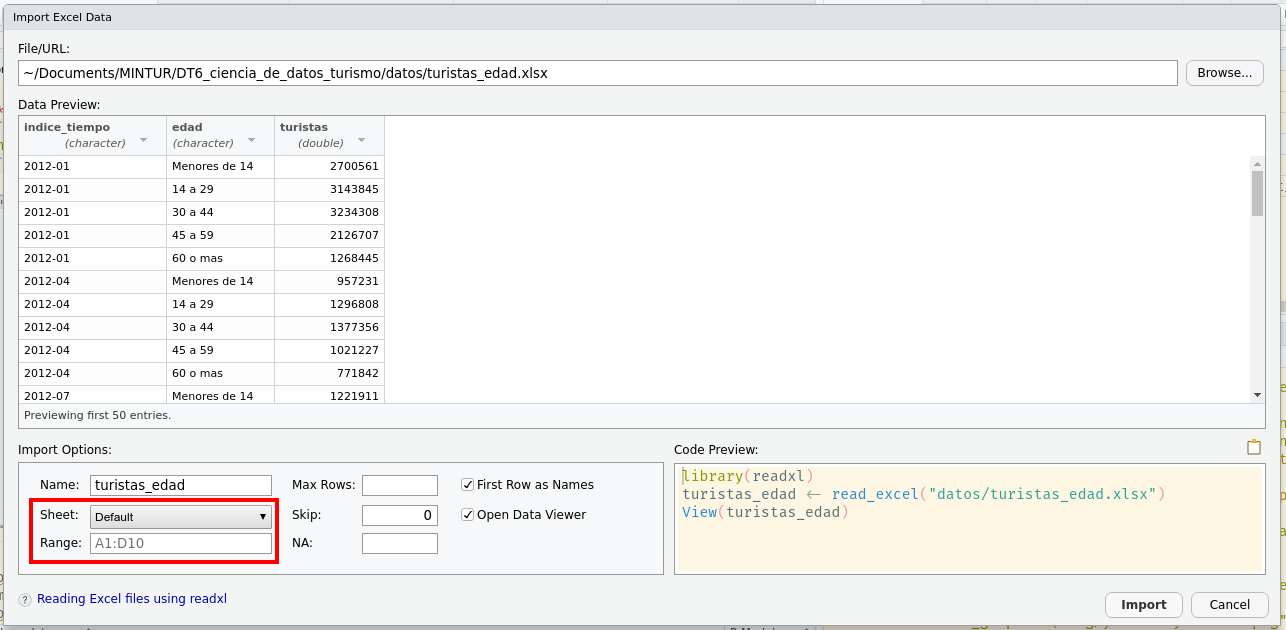
\includegraphics[width=1\linewidth]{img/importar-edad-xlsx} \end{center}

Notá que entre las opciones de abajo a la izquierda aparecen dos variables importantes.
Podés seleccionar de qué hoja leer los datos y qué rango usar.
Esto seguro que te va a ser muy útil para esos archivos de Excel con múltiples tablas en un archivo, o incluso múltiples tablas en cada hoja!

En este caso turistas\_edad.xlsx es un Excel buena onda, y el código para leer los datos es muy simple:

\begin{Shaded}
\begin{Highlighting}[]
\FunctionTok{library}\NormalTok{(readxl)}
\NormalTok{turistas\_edad }\OtherTok{\textless{}{-}} \FunctionTok{read\_excel}\NormalTok{(}\StringTok{"datos/turistas\_edad.xlsx"}\NormalTok{)}
\end{Highlighting}
\end{Shaded}

Con la función \texttt{str()} podés confirmar que los datos leídos son los mismos que para el csv.

\begin{Shaded}
\begin{Highlighting}[]
\FunctionTok{str}\NormalTok{(turistas\_edad)}
\end{Highlighting}
\end{Shaded}

\begin{verbatim}
## tibble [180 x 3] (S3: tbl_df/tbl/data.frame)
##  $ indice_tiempo: chr [1:180] "2012-01" "2012-01" "2012-01" "2012-01" ...
##  $ edad         : chr [1:180] "Menores de 14" "14 a 29" "30 a 44" "45 a 59" ...
##  $ turistas     : num [1:180] 2700561 3143845 3234308 2126707 1268445 ...
\end{verbatim}

\textbf{Desafío: Lee un archivo}

\begin{enumerate}
\def\labelenumi{\arabic{enumi}.}
\tightlist
\item
  Lee el archivo \texttt{turistas\_edad.xlsx}, pero solo las primeras 30 lineas
\item
  ¿Qué cambió en código que devuelve RStudio?
\item
  Revisa la documentación de la función \texttt{read\_excel()} para identificar otros argumentos que puedan resultarte útiles.
\end{enumerate}

\hypertarget{manipulaciuxf3n-de-datos-ordenados}{%
\chapter{Manipulación de datos ordenados}\label{manipulaciuxf3n-de-datos-ordenados}}

El paquete \textbf{dplyr} provee una enorme cantidad de funciones útiles para manipular y analizar datos de manera intuitiva y expresiva.

El espíritu detrás de dplyr es que la enorme mayoría de los análisis, por más complicados que sean, involucran combinar y encadenar una serie relativamente acotada de acciones (o verbos).
En este curso vamos a centrarnos las cinco más comunes:

\begin{itemize}
\tightlist
\item
  \texttt{select()}: selecciona columnas de una tabla.
\item
  \texttt{filter()}: selecciona (o filtra) filas de una tabla a partir de una o más condiciones lógicas.
\item
  \texttt{group\_by()}: agrupa una tabla en base al valor de una o más columnas.
\item
  \texttt{mutate()}: agrega nuevas columnas a una tabla.
\item
  \texttt{summarise()}: calcula estadísticas para cada grupo de una tabla.
\end{itemize}

\textbf{dplyr y tablas dinámicas:}

A grosso modo, las operaciones de dplyr permiten hacer en R lo que se hace en tablas dinámicas (pivot tables) en Excel.
\texttt{filter()} vendría a ser como la sección de ``Filtros'', \texttt{group\_by()}, la sección de ``Filas'', \texttt{select()}, la sección de ``Columnas'' y \texttt{summarise()}, la parte de ``Valores''.

\textbf{Primer desafío:}

Te dieron una tabla con datos de cantidad mensual de visitantes residentes y visitantes no residentes para cada provincia.
Las columnas son: \texttt{año}, \texttt{mes}, \texttt{provincia}, \texttt{visitantes\_residentes} y \texttt{visitantes\_no\_residentes}.
En base a esos datos, te piden que calcules la proporción promedio de visitantes que son residentes para cada provincia en enero.

¿En qué orden ejecutarías estos pasos para obtener el resultado deseado?

\begin{itemize}
\tightlist
\item
  usar \texttt{summarise()} para calcular la estadística \texttt{mean(proporcion\_residentes)} para cada \texttt{provincia}
\item
  usar \texttt{group\_by()} para agrupar por la columna \texttt{provincia}
\item
  usar \texttt{mutate()} para agregar una columna llamada \texttt{proporcion\_residentes} que sea \texttt{visitantes\_residentes/(visitantes\_residentes\ +\ visitantes\_no\_residentes)}.
\item
  usar \texttt{filter()} para seleccionar solo las filas donde la columna \texttt{mes} es igual a 1.
\end{itemize}

Para usar dplyr primero hay que instalarlo (esto hay que hacerlo una sola vez por computadora) con el comando:

\begin{Shaded}
\begin{Highlighting}[]
\FunctionTok{install.packages}\NormalTok{(}\StringTok{"dplyr"}\NormalTok{)}
\end{Highlighting}
\end{Shaded}

y luego cargarlo en memoria con

\begin{Shaded}
\begin{Highlighting}[]
\FunctionTok{library}\NormalTok{(dplyr)}
\end{Highlighting}
\end{Shaded}

Volvé a cargar los datos de turistas por edad (para un recordatorio, podés ir a \href{lectura-de-datos-ordenados.html}{Lectura de datos ordenados}):

\begin{Shaded}
\begin{Highlighting}[]
\FunctionTok{library}\NormalTok{(readr)}
\NormalTok{turistas\_edad }\OtherTok{\textless{}{-}} \FunctionTok{read\_csv}\NormalTok{(}\StringTok{"datos/turistas\_edad.csv"}\NormalTok{)}
\end{Highlighting}
\end{Shaded}

\hypertarget{seleccionando-columnas-con-select}{%
\section{\texorpdfstring{Seleccionando columnas con \texttt{select()}}{Seleccionando columnas con select()}}\label{seleccionando-columnas-con-select}}

Para quedarse únicamente con las columnas de índice de tiempo y turistas, usá \texttt{select()}

\begin{Shaded}
\begin{Highlighting}[]
\FunctionTok{select}\NormalTok{(turistas\_edad, indice\_tiempo, turistas)}
\end{Highlighting}
\end{Shaded}

\begin{verbatim}
## # A tibble: 180 x 2
##    indice_tiempo turistas
##    <chr>            <dbl>
##  1 2012-01        2700561
##  2 2012-01        3143845
##  3 2012-01        3234308
##  4 2012-01        2126707
##  5 2012-01        1268445
##  6 2012-04         957231
##  7 2012-04        1296808
##  8 2012-04        1377356
##  9 2012-04        1021227
## 10 2012-04         771842
## # ... with 170 more rows
\end{verbatim}

¿Dónde quedó este resultado?
Si te fijás en la tabla \texttt{turistas\_edad}, su formato no cambió, sigue teniendo todas las columnas originales a pesar de nuestro select:

\begin{Shaded}
\begin{Highlighting}[]
\NormalTok{turistas\_edad}
\end{Highlighting}
\end{Shaded}

\begin{verbatim}
## # A tibble: 180 x 3
##    indice_tiempo edad          turistas
##    <chr>         <chr>            <dbl>
##  1 2012-01       Menores de 14  2700561
##  2 2012-01       14 a 29        3143845
##  3 2012-01       30 a 44        3234308
##  4 2012-01       45 a 59        2126707
##  5 2012-01       60 o mas       1268445
##  6 2012-04       Menores de 14   957231
##  7 2012-04       14 a 29        1296808
##  8 2012-04       30 a 44        1377356
##  9 2012-04       45 a 59        1021227
## 10 2012-04       60 o mas        771842
## # ... with 170 more rows
\end{verbatim}

\texttt{select()} y el resto de las funciones de dplyr siempre generan una nueva tabla y nunca modifican la tabla original.
Para guardar la tabla con las dos columnas \texttt{indice\_tiempo} y \texttt{turistas} tenés que asignar el resultado a una nueva variable.

\begin{Shaded}
\begin{Highlighting}[]
\NormalTok{turistas\_edad2 }\OtherTok{\textless{}{-}} \FunctionTok{select}\NormalTok{(turistas\_edad, indice\_tiempo, turistas)}
\NormalTok{turistas\_edad2}
\end{Highlighting}
\end{Shaded}

\begin{verbatim}
## # A tibble: 180 x 2
##    indice_tiempo turistas
##    <chr>            <dbl>
##  1 2012-01        2700561
##  2 2012-01        3143845
##  3 2012-01        3234308
##  4 2012-01        2126707
##  5 2012-01        1268445
##  6 2012-04         957231
##  7 2012-04        1296808
##  8 2012-04        1377356
##  9 2012-04        1021227
## 10 2012-04         771842
## # ... with 170 more rows
\end{verbatim}

\begin{figure}
\centering
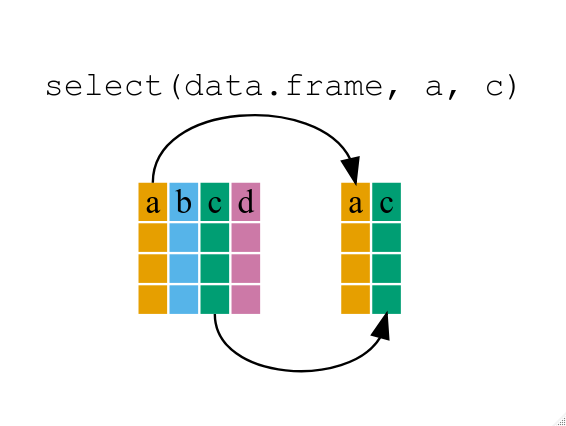
\includegraphics{img/dplyr-select.png}
\caption{Cómo funciona \texttt{select()}}
\end{figure}

\hypertarget{filtrando-filas-con-filter}{%
\section{\texorpdfstring{Filtrando filas con \texttt{filter()}}{Filtrando filas con filter()}}\label{filtrando-filas-con-filter}}

Ahora podés usar \texttt{filter()} para quedarte con sólo unas filas.
Por ejemplo, para quedarse con los turistas menores de 14 años

\begin{Shaded}
\begin{Highlighting}[]
\FunctionTok{filter}\NormalTok{(turistas\_edad, edad }\SpecialCharTok{==} \StringTok{"Menores de 14"}\NormalTok{)}
\end{Highlighting}
\end{Shaded}

\begin{verbatim}
## # A tibble: 36 x 3
##    indice_tiempo edad          turistas
##    <chr>         <chr>            <dbl>
##  1 2012-01       Menores de 14  2700561
##  2 2012-04       Menores de 14   957231
##  3 2012-07       Menores de 14  1221911
##  4 2012-10       Menores de 14  1172970
##  5 2013-01       Menores de 14  2604040
##  6 2013-04       Menores de 14   942360
##  7 2013-07       Menores de 14  1341895
##  8 2013-10       Menores de 14  1382380
##  9 2014-01       Menores de 14  2706215
## 10 2014-04       Menores de 14  1006238
## # ... with 26 more rows
\end{verbatim}

La mayoría de los análisis consisten en varios pasos que van generando tablas intermedias (en el primer desafío usaste 4 pasos para calcular la proporción media de visitantes residentes)
La única tabla que te interesa es la última, por lo que ir asignando variables nuevas en cada paso intermedio es tedioso y poco práctico.
Para eso se usa el operador `pipe' (\texttt{\%\textgreater{}\%}).

El operador `pipe' (\texttt{\%\textgreater{}\%}) agarra el resultado de una función y se lo pasa a la siguiente.
Esto permite escribir el código como una cadena de funciones que van operando sobre el resultado de la anterior.

Las dos operaciones anteriores (seleccionar tres columnas y luego filtrar las filas correspondientes a Argentina) se pueden escribir uno después del otro y sin asignar los resultados intermedios a nuevas variables de esta forma:

\begin{Shaded}
\begin{Highlighting}[]
\NormalTok{turistas\_edad }\SpecialCharTok{\%\textgreater{}\%} 
  \FunctionTok{filter}\NormalTok{(edad }\SpecialCharTok{==} \StringTok{"Menores de 14"}\NormalTok{) }\SpecialCharTok{\%\textgreater{}\%} 
  \FunctionTok{select}\NormalTok{(indice\_tiempo, turistas)}
\end{Highlighting}
\end{Shaded}

\begin{verbatim}
## # A tibble: 36 x 2
##    indice_tiempo turistas
##    <chr>            <dbl>
##  1 2012-01        2700561
##  2 2012-04         957231
##  3 2012-07        1221911
##  4 2012-10        1172970
##  5 2013-01        2604040
##  6 2013-04         942360
##  7 2013-07        1341895
##  8 2013-10        1382380
##  9 2014-01        2706215
## 10 2014-04        1006238
## # ... with 26 more rows
\end{verbatim}

La forma de ``leer'' esto es ``Tomá la variable \texttt{turistas\_edad}, \textbf{después} aplicale \texttt{s\ filter(edad\ ==\ "Menores\ de\ 14")}, \textbf{después} aplicale \texttt{fselect(indice\_tiempo,\ turistas)}''.

Cómo vimos, el primer argumento de todas las funciones de dplyr es el data frame sobre el cual van a operar, pero notá que en las líneas con \texttt{select()} y \texttt{filter()} no escribís la tabla explícitamente.\\
Esto es porque la pipe implícitamente pasa el resultado de las líneas anteriores como el primer argumento de la función siguiente.

Toma el data frame \texttt{turistas\_edad} y se lo pasa al primer argumento de \texttt{select()}.
Luego el data frame resultante de esa operación pasa como el primer argumento de la función \texttt{filter()} gracias al \texttt{\%\textgreater{}\%}.

\textbf{Tip:}

En RStudio podés escribir \texttt{\%\textgreater{}\%} usando el atajo de teclado Ctr + Shift + M.
¡Probalo!

\textbf{Desafío:}

Completá esta cadena para producir una tabla que contenga los datos de turistas de 60 o más años

\begin{Shaded}
\begin{Highlighting}[]
\NormalTok{turistas\_edad }\SpecialCharTok{\%\textgreater{}\%} 
  \FunctionTok{filter}\NormalTok{(edad }\SpecialCharTok{==}\NormalTok{ \_\_\_) }\SpecialCharTok{\%\textgreater{}\%} 
  \FunctionTok{select}\NormalTok{(\_\_\_\_\_, \_\_\_\_)}
\end{Highlighting}
\end{Shaded}

\hypertarget{agrupando-y-reduciendo-con-group_by-summarise}{%
\section{\texorpdfstring{Agrupando y reduciendo con \texttt{group\_by()\ \%\textgreater{}\%\ summarise()}}{Agrupando y reduciendo con group\_by() \%\textgreater\% summarise()}}\label{agrupando-y-reduciendo-con-group_by-summarise}}

Si querés calcular la cantidad promedio de turistas por cada rango de edad, tenés que usar el combo \texttt{group\_by()\ \%\textgreater{}\%\ summarise()}.
Es decir, primero agrupar la tabla según la columna \texttt{edad} y luego calcular el promedio de \texttt{turistas} para cada grupo.

Para agrupar la tabla países según el continente usamos el siguiente código:

\begin{Shaded}
\begin{Highlighting}[]
\NormalTok{turistas\_edad }\SpecialCharTok{\%\textgreater{}\%} 
  \FunctionTok{group\_by}\NormalTok{(edad) }
\end{Highlighting}
\end{Shaded}

\begin{verbatim}
## # A tibble: 180 x 3
## # Groups:   edad [5]
##    indice_tiempo edad          turistas
##    <chr>         <chr>            <dbl>
##  1 2012-01       Menores de 14  2700561
##  2 2012-01       14 a 29        3143845
##  3 2012-01       30 a 44        3234308
##  4 2012-01       45 a 59        2126707
##  5 2012-01       60 o mas       1268445
##  6 2012-04       Menores de 14   957231
##  7 2012-04       14 a 29        1296808
##  8 2012-04       30 a 44        1377356
##  9 2012-04       45 a 59        1021227
## 10 2012-04       60 o mas        771842
## # ... with 170 more rows
\end{verbatim}

A primera vista parecería que la función no hizo nada, pero fijate que el resultado ahora dice que tiene grupos (``Groups:''), y nos dice qué columna es la que agrupa los datos (``edad'') y cuántos grupos hay (``5'').
Las operaciones subsiguientes que le hagamos a esta tabla van a hacerse \emph{para cada grupo}.

Para ver esto en acción, usá \texttt{summarise()} para computar el promedio de turistas

\begin{Shaded}
\begin{Highlighting}[]
\NormalTok{turistas\_edad }\SpecialCharTok{\%\textgreater{}\%} 
  \FunctionTok{group\_by}\NormalTok{(edad) }\SpecialCharTok{\%\textgreater{}\%} 
  \FunctionTok{summarise}\NormalTok{(}\AttributeTok{turistas\_promedio =} \FunctionTok{mean}\NormalTok{(turistas))}
\end{Highlighting}
\end{Shaded}

\begin{verbatim}
## # A tibble: 5 x 2
##   edad          turistas_promedio
##   <chr>                     <dbl>
## 1 14 a 29                1440779.
## 2 30 a 44                1530064.
## 3 45 a 59                1242697.
## 4 60 o mas               1033486.
## 5 Menores de 14          1368313.
\end{verbatim}

¡Tadá!
\texttt{summarise()} devuelve una tabla con una columna para la edad y otra nueva, llamada ``turistas\_promedio'' que contiene el promedio de \texttt{turistas} para cada grupo.
Esta operación es equivalente a esta tabla dinámica en Excel:

\textbf{rehacer el video}

\texttt{group\_by()} permite agrupar en base a múltiples columnas y \texttt{summarise()} permite generar múltiples columnas de resumen.
El siguiente código calcula la cantidad promedio de turistas y su desvío estándar para cada continente y cada año.

\begin{Shaded}
\begin{Highlighting}[]
\NormalTok{turistas\_edad }\SpecialCharTok{\%\textgreater{}\%} 
  \FunctionTok{group\_by}\NormalTok{(edad, }\AttributeTok{mes =} \FunctionTok{substr}\NormalTok{(indice\_tiempo, }\DecValTok{6}\NormalTok{, }\DecValTok{7}\NormalTok{)) }\SpecialCharTok{\%\textgreater{}\%} 
  \FunctionTok{summarise}\NormalTok{(}\AttributeTok{turistas\_promedio =} \FunctionTok{mean}\NormalTok{(turistas),}
            \AttributeTok{turistas\_desvio =} \FunctionTok{sd}\NormalTok{(turistas))}
\end{Highlighting}
\end{Shaded}

\begin{verbatim}
## `summarise()` has grouped output by 'edad'. You can override using the `.groups` argument.
\end{verbatim}

\begin{verbatim}
## # A tibble: 20 x 4
## # Groups:   edad [5]
##    edad          mes   turistas_promedio turistas_desvio
##    <chr>         <chr>             <dbl>           <dbl>
##  1 14 a 29       01             2432791.         439326.
##  2 14 a 29       04              889256.         421702.
##  3 14 a 29       07             1239470.         508496.
##  4 14 a 29       10             1201600.         310893.
##  5 30 a 44       01             2571253.         411656.
##  6 30 a 44       04              954923.         419869.
##  7 30 a 44       07             1289021.         454895.
##  8 30 a 44       10             1305058.         301415.
##  9 45 a 59       01             1955239.         119285.
## 10 45 a 59       04              826473.         319558.
## 11 45 a 59       07             1088687.         421866.
## 12 45 a 59       10             1100391.         245137.
## 13 60 o mas      01             1410029.         196945.
## 14 60 o mas      04              827572.         323722.
## 15 60 o mas      07              931603.         364683.
## 16 60 o mas      10              964739.         278363.
## 17 Menores de 14 01             2452844.         284910.
## 18 Menores de 14 04              698172.         307543.
## 19 Menores de 14 07             1126737.         409562.
## 20 Menores de 14 10             1195499          273635.
\end{verbatim}

\textbf{Tip:}

Este código usa \texttt{substr(indice\_tiempo,\ 6,\ 7)} para definir el mes.
Esta línea lo que hace es quedarse con el texto de \texttt{indice\_tiempo} que está entre la posición 6 y la 7.
De esta manera, del texto \texttt{"2012-01"} se queda con ``\texttt{01}'', que representa el mes.

Esta no es la mejor manera de trabajar con fechas, pero es suficiente por ahora.

El resultado va a siempre ser una tabla con la misma cantidad de filas que grupos y una cantidad de columnas igual a la cantidad de columnas usadas para agrupar y los estadísticos computados.

\textbf{Desafío:}

¿Cuál te imaginás que va a ser el resultado del siguiente código?
¿Cuántas filas y columnas va a tener?
(Tratá de pensarlo antes de correrlo.)

\begin{Shaded}
\begin{Highlighting}[]
\NormalTok{turistas\_edad }\SpecialCharTok{\%\textgreater{}\%} 
   \FunctionTok{summarise}\NormalTok{(}\AttributeTok{turistas\_promedio =} \FunctionTok{mean}\NormalTok{(turistas))}
\end{Highlighting}
\end{Shaded}

El combo \texttt{group\_by()\ \%\textgreater{}\%\ summarise()} se puede resumir en esta figura.
Las filas de una tabla se dividen en grupos, y luego cada grupo se ``resume'' en una fila en función del estadístico usado.

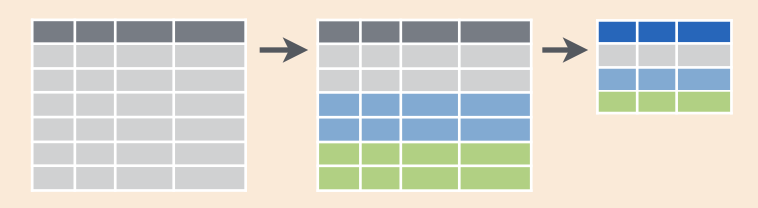
\includegraphics{img/group_by-summarize.png}

Al igual que hicimos ``cuentas'' usando algunas variables numéricas para obtener información nueva, también podemos utilizar variables categóricas.
No tiene sentido calcular \texttt{mean(edad)} ya que en esta tabla la edad está codificada como texto, pero tal vez te interese \emph{contar} la cantidad de observaciones por edad:

\begin{Shaded}
\begin{Highlighting}[]
\NormalTok{turistas\_edad }\SpecialCharTok{\%\textgreater{}\%} 
  \FunctionTok{group\_by}\NormalTok{(edad) }\SpecialCharTok{\%\textgreater{}\%} 
  \FunctionTok{summarise}\NormalTok{(}\AttributeTok{cantidad =} \FunctionTok{n}\NormalTok{())}
\end{Highlighting}
\end{Shaded}

\begin{verbatim}
## # A tibble: 5 x 2
##   edad          cantidad
##   <chr>            <int>
## 1 14 a 29             36
## 2 30 a 44             36
## 3 45 a 59             36
## 4 60 o mas            36
## 5 Menores de 14       36
\end{verbatim}

En este caso se ve que hay 36 observaciones (36 fechas) para todos los rangos etáreos.

\hypertarget{creando-nuevas-columnas-con-mutate}{%
\section{\texorpdfstring{Creando nuevas columnas con \texttt{mutate()}}{Creando nuevas columnas con mutate()}}\label{creando-nuevas-columnas-con-mutate}}

Todo esto está bien para hacer cálculos con columnas previamente existentes, pero muchas veces tenés que crear nuevas columnas.

La tabla \texttt{turistas\_edad} tiene información temporal codificada como texto en el formato ``año-mes''.
Sería mucho mejor que esté codificada como una fecha.
Una forma muy simple de convertir caracteres a fechas es usando el paquete \textbf{lubridate}.
Este paquete tiene un montón de funciones que te facilitan la vida al trabajar con fechas, pero en este caso vamos a usar la función \texttt{ym()} que transforma en fecha cualquier texto que tenga una fecha codificada con el año seguido del mes.

Para agregar una columna llamada \texttt{tiempo} a la tabla \texttt{turistas\_edad}, vamos a usar la función \texttt{mutate()}

\begin{Shaded}
\begin{Highlighting}[]
\NormalTok{turistas\_edad }\SpecialCharTok{\%\textgreater{}\%} 
  \FunctionTok{mutate}\NormalTok{(}\AttributeTok{tiempo =}\NormalTok{ lubridate}\SpecialCharTok{::}\FunctionTok{ym}\NormalTok{(indice\_tiempo))}
\end{Highlighting}
\end{Shaded}

\begin{verbatim}
## # A tibble: 180 x 4
##    indice_tiempo edad          turistas tiempo    
##    <chr>         <chr>            <dbl> <date>    
##  1 2012-01       Menores de 14  2700561 2012-01-01
##  2 2012-01       14 a 29        3143845 2012-01-01
##  3 2012-01       30 a 44        3234308 2012-01-01
##  4 2012-01       45 a 59        2126707 2012-01-01
##  5 2012-01       60 o mas       1268445 2012-01-01
##  6 2012-04       Menores de 14   957231 2012-04-01
##  7 2012-04       14 a 29        1296808 2012-04-01
##  8 2012-04       30 a 44        1377356 2012-04-01
##  9 2012-04       45 a 59        1021227 2012-04-01
## 10 2012-04       60 o mas        771842 2012-04-01
## # ... with 170 more rows
\end{verbatim}

¿Notás la diferencia entre la columna \texttt{indice\_tiempo} y \texttt{tiempo}?

Recordá que las funciones de dplyr nunca modifican la tabla original.
\texttt{mutate()} devolvió una nueva tabla que es igual a la tabla \texttt{turistas\_edad} pero con la columna ``tiempo'' agregada.
La tabla \texttt{turistas\_edad} sigue intacta.

\textbf{Tip:}

Para usar la función \texttt{ym()} del paquete lubridate el código de arriba usa \texttt{lubridate::ym()}.
Esta es una forma de usar funciones de paquetes sin tener que cargarlos con \texttt{library()}.

\hypertarget{desagrupando-con-ungroup}{%
\section{\texorpdfstring{Desagrupando con \texttt{ungroup()}}{Desagrupando con ungroup()}}\label{desagrupando-con-ungroup}}

En general, la mayoría de las funciones de dplyr ``entienden'' cuando una tabla está agrupada y realizan las operaciones para cada grupo.

\textbf{Desafío:}

¿Cuál de estos dos códigos agrega una columna llamada ``turistas\_promedio'' con la cantidad de turistas promedios para cada rango de dades?
¿Qué hace el otro?

\begin{Shaded}
\begin{Highlighting}[]
\NormalTok{turistas\_edad }\SpecialCharTok{\%\textgreater{}\%} 
  \FunctionTok{group\_by}\NormalTok{(edad) }\SpecialCharTok{\%\textgreater{}\%} 
  \FunctionTok{mutate}\NormalTok{(}\AttributeTok{turistas\_promedio =} \FunctionTok{mean}\NormalTok{(turistas)) }

\NormalTok{turistas\_edad }\SpecialCharTok{\%\textgreater{}\%} 
  \FunctionTok{mutate}\NormalTok{(}\AttributeTok{turistas\_promedio =} \FunctionTok{mean}\NormalTok{(turistas)) }
\end{Highlighting}
\end{Shaded}

En otras palabras, los resultados de \texttt{mutate()}, \texttt{filter()}, \texttt{summarise()} y otras funciones cambian según si la tabla está agrupada o no.
Como a veces uno se puede olvidar que quedaron grupos, es conveniente usar la función \texttt{ungroup()} una vez que dejás de trabajar con grupos:

\begin{Shaded}
\begin{Highlighting}[]
\NormalTok{turistas\_edad }\SpecialCharTok{\%\textgreater{}\%} 
  \FunctionTok{group\_by}\NormalTok{(edad) }\SpecialCharTok{\%\textgreater{}\%} 
  \FunctionTok{mutate}\NormalTok{(}\AttributeTok{turistas\_promedio =} \FunctionTok{mean}\NormalTok{(turistas)) }\SpecialCharTok{\%\textgreater{}\%} 
  \FunctionTok{ungroup}\NormalTok{()}
\end{Highlighting}
\end{Shaded}

\begin{verbatim}
## # A tibble: 180 x 4
##    indice_tiempo edad          turistas turistas_promedio
##    <chr>         <chr>            <dbl>             <dbl>
##  1 2012-01       Menores de 14  2700561          1368313.
##  2 2012-01       14 a 29        3143845          1440779.
##  3 2012-01       30 a 44        3234308          1530064.
##  4 2012-01       45 a 59        2126707          1242697.
##  5 2012-01       60 o mas       1268445          1033486.
##  6 2012-04       Menores de 14   957231          1368313.
##  7 2012-04       14 a 29        1296808          1440779.
##  8 2012-04       30 a 44        1377356          1530064.
##  9 2012-04       45 a 59        1021227          1242697.
## 10 2012-04       60 o mas        771842          1033486.
## # ... with 170 more rows
\end{verbatim}

\hypertarget{manipulaciuxf3n-de-datos-ordenados-usando-dplyr-y-tidyr-ii}{%
\chapter{Manipulación de datos ordenados usando \{dplyr\} y \{tidyr\} II}\label{manipulaciuxf3n-de-datos-ordenados-usando-dplyr-y-tidyr-ii}}

En \href{04-lectura-datos.html\#Formatos_de_tablas}{la última sección de lectura de datos} viste el concepto de datos ``anchos'' y ``largos''.

Los datos en formato ``largo'' o ``tidy'', son aquellos en los cuales:

\begin{itemize}
\tightlist
\item
  cada fila es una observación
\item
  cada columna es una variable
\end{itemize}

En el formato ``ancho'' es un poco más complejo de definirlo pero la idea general es que:

\begin{itemize}
\tightlist
\item
  cada fila es un ``item''
\item
  cada columna es una variable
\end{itemize}

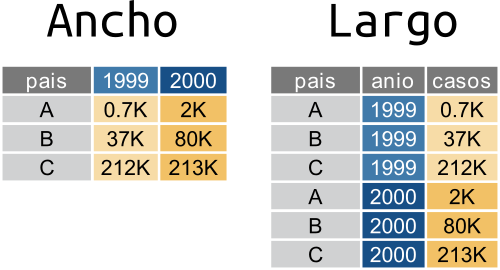
\includegraphics{img/largo-ancho.png}

Una tabla en formato largo va a tener una cierta cantidad de columnas que cumplen el rol de \emph{identificadores} y cuya combinación identifican una única observación y una única columna con el valor de la observación.
En el ejemplo de arriba, \texttt{pais} y \texttt{anio} son las columnas identificadoras y \texttt{casos} es la columna que contiene el valor de las observaciones.

En una tabla ancha, cada observación única se identifica a partir de la intersección de filas y columnas.
En el ejemplo, los países están en las filas y los años en las columnas.

En general, el formato ancho es más compacto y legible por humanos mientras que el largo es más fácil de manejar con la computadora.
Si te fijás en las tablas de arriba, es más fácil comparar los valores entre países y entre años en la tabla ancha.
Pero el nombre de las columnas (``1999'', ``2000'') en realidad ¡son datos!
Además este formato se empieza a complicar en cuanto hay más de dos identificadores.

Un mismo set de datos puede ser representado de forma completamente ``larga'', completamente ``ancha'' o --lo que es más común-- en un formato intermedio pero no existe una forma ``correcta'' de organizar los datos; cada una tiene sus ventajas y desventajas.
Por esto es que es muy normal que durante un análisis los datos vayan y vuelvan entre distintos formatos dependiendo de los métodos estadísticos que se le aplican.
Entonces, aprender a transformar datos anchos en largos y viceversa es un habilidad muy útil.

\textbf{Desafío}

En las tablas de ejemplo cada país tiene el un valor observado de ``casos'' para cada año.
¿Cómo agregarías una nueva variable con información sobre ``precios''?
Dibujá un esquema en papel y lápiz en formato ancho y uno en formato largo.
¿En qué formato es más ``natural'' esa extensión?

En esta sección vas a usar el paquete \{tidyr\} para manipular datos.
Si no lo tenés instalado, instalalo con el comando:

\begin{Shaded}
\begin{Highlighting}[]
\FunctionTok{install.packages}\NormalTok{(}\StringTok{"tidyr"}\NormalTok{)}
\end{Highlighting}
\end{Shaded}

(como siempre, recordá que esto hay que hacerlo una única vez)

Y luego cargá \{tidyr\} y \{dplyr\} (que usaste en \href{05-dplyr-I.html}{una sección anterior}) con:

\begin{Shaded}
\begin{Highlighting}[]
\FunctionTok{library}\NormalTok{(tidyr)}
\FunctionTok{library}\NormalTok{(dplyr)}
\end{Highlighting}
\end{Shaded}

\hypertarget{de-ancho-a-largo-con-pivot_longer}{%
\section{\texorpdfstring{De ancho a largo con \texttt{pivot\_longer()}}{De ancho a largo con pivot\_longer()}}\label{de-ancho-a-largo-con-pivot_longer}}

En secciones anteriores usaste una versión de los datos de \href{https://www.gapminder.org/}{gapminder}.
Ahora vas a leer los datos en su formato original:

\begin{Shaded}
\begin{Highlighting}[]
\NormalTok{paises\_ancho }\OtherTok{\textless{}{-}}\NormalTok{ readr}\SpecialCharTok{::}\FunctionTok{read\_csv}\NormalTok{(}\StringTok{"datos/paises\_ancho.csv"}\NormalTok{)}
\end{Highlighting}
\end{Shaded}

\begin{verbatim}
## Rows: 142 Columns: 38
\end{verbatim}

\begin{verbatim}
## -- Column specification --------------------------------------------------------
## Delimiter: ","
## chr  (2): continente, pais
## dbl (36): pib_per_capita_1952, pib_per_capita_1957, pib_per_capita_1962, pib...
\end{verbatim}

\begin{verbatim}
## 
## i Use `spec()` to retrieve the full column specification for this data.
## i Specify the column types or set `show_col_types = FALSE` to quiet this message.
\end{verbatim}

\begin{Shaded}
\begin{Highlighting}[]
\NormalTok{paises\_ancho}
\end{Highlighting}
\end{Shaded}

\begin{verbatim}
## # A tibble: 142 x 38
##    continente pais                     pib_per_capita_~ pib_per_capita_~ pib_per_capita_~
##    <chr>      <chr>                               <dbl>            <dbl>            <dbl>
##  1 Africa     Algeria                             2449.            3014.            2551.
##  2 Africa     Angola                              3521.            3828.            4269.
##  3 Africa     Benin                               1063.             960.             949.
##  4 Africa     Botswana                             851.             918.             984.
##  5 Africa     Burkina Faso                         543.             617.             723.
##  6 Africa     Burundi                              339.             380.             355.
##  7 Africa     Cameroon                            1173.            1313.            1400.
##  8 Africa     Central African Republic            1071.            1191.            1193.
##  9 Africa     Chad                                1179.            1308.            1390.
## 10 Africa     Comoros                             1103.            1211.            1407.
## # ... with 132 more rows, and 33 more variables: pib_per_capita_1967 <dbl>,
## #   pib_per_capita_1972 <dbl>, pib_per_capita_1977 <dbl>,
## #   pib_per_capita_1982 <dbl>, pib_per_capita_1987 <dbl>,
## #   pib_per_capita_1992 <dbl>, pib_per_capita_1997 <dbl>,
## #   pib_per_capita_2002 <dbl>, pib_per_capita_2007 <dbl>,
## #   esperanza_de_vida_1952 <dbl>, esperanza_de_vida_1957 <dbl>,
## #   esperanza_de_vida_1962 <dbl>, esperanza_de_vida_1967 <dbl>, ...
\end{verbatim}

¿Notaste que en el código anterior no usaste \texttt{library(readr)} para cargar el paquete y luego leer?
Con la notación \texttt{paquete::funcion()} podés acceder a las funciones de un paquete sin tener que cargarlo.
Es una buena forma de no tener que cargar un montón de paquetes innecesarios si vas a correr una única función de un paquete pocas veces.

Esta tabla, increíblemente ancha, es muy difícil de manejar.
Por ejemplo, es imposible hacer una serie de tiempo de una variable, o calcular el promedio por variable y país; ni hablar de calcular una regresión lineal.

Para convertirlo en una tabla más larga, se usa \texttt{pivot\_longer()} (``longer'' es ``más largo'' en inglés):

\begin{Shaded}
\begin{Highlighting}[]
\NormalTok{paises\_largo }\OtherTok{\textless{}{-}} \FunctionTok{pivot\_longer}\NormalTok{(paises\_ancho,}
                             \AttributeTok{cols =} \FunctionTok{c}\NormalTok{(}\FunctionTok{starts\_with}\NormalTok{(}\StringTok{\textquotesingle{}pob\textquotesingle{}}\NormalTok{), }
                                      \FunctionTok{starts\_with}\NormalTok{(}\StringTok{\textquotesingle{}esperanza\textquotesingle{}}\NormalTok{), }
                                      \FunctionTok{starts\_with}\NormalTok{(}\StringTok{\textquotesingle{}pib\_per\textquotesingle{}}\NormalTok{)),}
                             \AttributeTok{names\_to =} \StringTok{"variable\_anio"}\NormalTok{, }
                             \AttributeTok{values\_to =} \StringTok{"valor"}
\NormalTok{)}
\NormalTok{paises\_largo}
\end{Highlighting}
\end{Shaded}

\begin{verbatim}
## # A tibble: 5,112 x 4
##    continente pais    variable_anio     valor
##    <chr>      <chr>   <chr>             <dbl>
##  1 Africa     Algeria poblacion_1952  9279525
##  2 Africa     Algeria poblacion_1957 10270856
##  3 Africa     Algeria poblacion_1962 11000948
##  4 Africa     Algeria poblacion_1967 12760499
##  5 Africa     Algeria poblacion_1972 14760787
##  6 Africa     Algeria poblacion_1977 17152804
##  7 Africa     Algeria poblacion_1982 20033753
##  8 Africa     Algeria poblacion_1987 23254956
##  9 Africa     Algeria poblacion_1992 26298373
## 10 Africa     Algeria poblacion_1997 29072015
## # ... with 5,102 more rows
\end{verbatim}

El primer argumento de\texttt{pivot\_longer()} es la tabla que va a modificar: \texttt{paises\_ancho}.
El segundo argumento se llama \texttt{cols} y es un vector con las columnas que tienen los valores a ``alargar''.
Podría ser un vector escrito a mano (algo como \texttt{c("pib\_per\_capita\_1952",\ "pib\_per\_capita\_1957"...)}) pero con más de 30 columnas, escribir todo eso sería tedioso y probablemente estaría lleno de errores.
Por eso \{tidyr\} provee funciones de ayuda para seleccionar columnas en base a patrones.
El código de arriba usa \texttt{starts\_with()} que, como su nombre en inglés lo indica, selecciona las columnas que \emph{empiezan con} una determinada cadena de caracteres.
El vector \texttt{c(starts\_with(\textquotesingle{}pob\textquotesingle{}),\ starts\_with(\textquotesingle{}esperanza\textquotesingle{}),\ starts\_with(\textquotesingle{}pib\_per\textquotesingle{}))} le dice a \texttt{pivot\_longer()} que seleccione las columnas que empieza con ``pob'', las que empiezan con ``esperanza'' y las que empiezan con ``pib\_per''.

Estas funciones accesorias para seleccionar muchas funciones se llaman ``tidyselect''.
Si querés leer más detalles de las distintas formas que podés seleccionar variables leé la documentación usando \texttt{?tidyselect::language}.

El tercer y cuarto argumento son los nombres de las columnas de ``nombre'' y de ``valor'' que va a tener la nueva tabla.
Como la nueva columna de identificación tiene los datos de la variable y el año a medir, ``variable\_anio'' es un buen nombre.
Y la columna de valor va a tener\ldots{} bueno, el valor.

Tomate un momento para visualizar lo que acaba de pasar.
La tabla ancha tenía un montón de columnas con distintos datos.
Ahora estos datos están uno arriba de otro en la columna ``valor'', pero para identificar el nombre de la columna de la cual vinieron, se agrega la columna ``variable\_anio''.

\begin{figure}
\centering
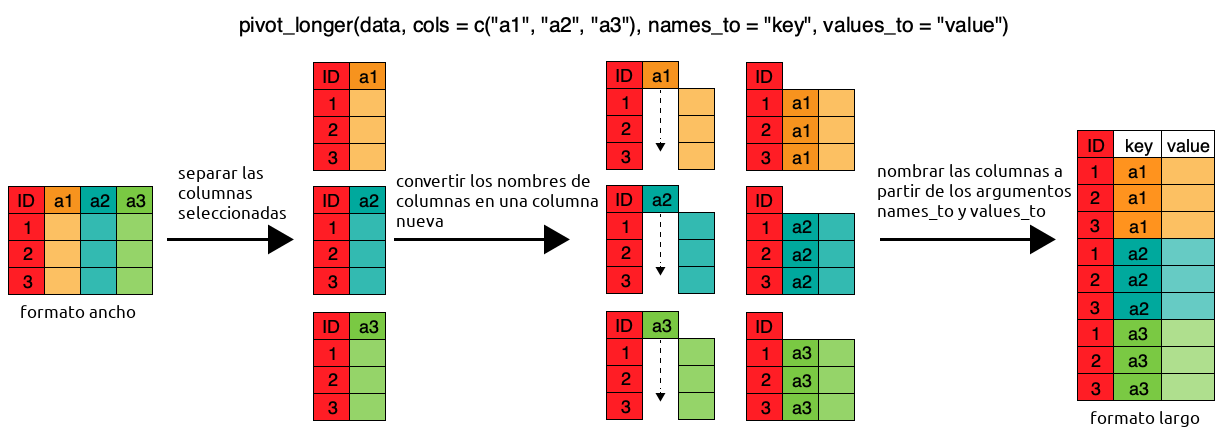
\includegraphics{img/ancho-a-largo.png}
\caption{Proceso de largo a ancho}
\end{figure}

La columna \texttt{variable\_anio} todavía no es muy útil porque contiene 2 datos, la variable (población, expectativa de vida o PBI per cápita) y el año.
Sería mejor separar esta información en dos columnas llamadas ``variable'' y ``anio''.
Para eso está la función \texttt{separate()}.

\begin{Shaded}
\begin{Highlighting}[]
\FunctionTok{separate}\NormalTok{(paises\_largo, }
         \AttributeTok{col =}\NormalTok{ variable\_anio, }
         \AttributeTok{into =} \FunctionTok{c}\NormalTok{(}\StringTok{"variable"}\NormalTok{, }\StringTok{"anio"}\NormalTok{), }
         \AttributeTok{sep =} \SpecialCharTok{{-}}\DecValTok{4}\NormalTok{)}
\end{Highlighting}
\end{Shaded}

\begin{verbatim}
## # A tibble: 5,112 x 5
##    continente pais    variable   anio     valor
##    <chr>      <chr>   <chr>      <chr>    <dbl>
##  1 Africa     Algeria poblacion_ 1952   9279525
##  2 Africa     Algeria poblacion_ 1957  10270856
##  3 Africa     Algeria poblacion_ 1962  11000948
##  4 Africa     Algeria poblacion_ 1967  12760499
##  5 Africa     Algeria poblacion_ 1972  14760787
##  6 Africa     Algeria poblacion_ 1977  17152804
##  7 Africa     Algeria poblacion_ 1982  20033753
##  8 Africa     Algeria poblacion_ 1987  23254956
##  9 Africa     Algeria poblacion_ 1992  26298373
## 10 Africa     Algeria poblacion_ 1997  29072015
## # ... with 5,102 more rows
\end{verbatim}

El primer argumento, como siempre, es la tabla a procesar.
El segundo, \texttt{col}, es la columna a separar en dos (o más) columnas nuevas.
El tercero, \texttt{into} es el nombre de las nuevas columnas que \texttt{separate()} va a crear.
El último argumento es \texttt{sep} que define cómo realizar la separación.
Por defecto, \texttt{sep} es una \href{https://es.wikipedia.org/wiki/Expresi\%C3\%B3n_regular}{expresión regular} que captura cualquier caracter no alfanumérico.
En el caso de \texttt{variable\_anio} no sirve, porque para valores como \texttt{"esperanza\_de\_vida\_1952"}, separaría en \texttt{"esperanza"}, \texttt{"de"}, \texttt{"vida"} y \texttt{"1952"}.
Como el año tiene siempre 4 caracteres, una solución simple es usar \texttt{sep\ =\ -4}, que significa que la separación es 4 caracteres contando desde el final.

Habrás notado un problema.
El texto en la columnas \texttt{variable} todavía tiene un ``\_'' al final.
Podrías usar \texttt{mutate()} y un poco de funciones de manipulación de caracteres para quitarlo, pero hay una forma un poco más simple y es separando la columna \texttt{variable\_anio} en tres, incluyendo una columna con el guión:

\begin{Shaded}
\begin{Highlighting}[]
\NormalTok{paises\_largo }\OtherTok{\textless{}{-}} \FunctionTok{separate}\NormalTok{(paises\_largo, }
         \AttributeTok{col =}\NormalTok{ variable\_anio, }
         \AttributeTok{into =} \FunctionTok{c}\NormalTok{(}\StringTok{"variable"}\NormalTok{, }\StringTok{"guion"}\NormalTok{, }\StringTok{"anio"}\NormalTok{), }
         \AttributeTok{sep =} \FunctionTok{c}\NormalTok{(}\SpecialCharTok{{-}}\DecValTok{5}\NormalTok{, }\SpecialCharTok{{-}}\DecValTok{4}\NormalTok{))}
\NormalTok{paises\_largo}
\end{Highlighting}
\end{Shaded}

\begin{verbatim}
## # A tibble: 5,112 x 6
##    continente pais    variable  guion anio     valor
##    <chr>      <chr>   <chr>     <chr> <chr>    <dbl>
##  1 Africa     Algeria poblacion _     1952   9279525
##  2 Africa     Algeria poblacion _     1957  10270856
##  3 Africa     Algeria poblacion _     1962  11000948
##  4 Africa     Algeria poblacion _     1967  12760499
##  5 Africa     Algeria poblacion _     1972  14760787
##  6 Africa     Algeria poblacion _     1977  17152804
##  7 Africa     Algeria poblacion _     1982  20033753
##  8 Africa     Algeria poblacion _     1987  23254956
##  9 Africa     Algeria poblacion _     1992  26298373
## 10 Africa     Algeria poblacion _     1997  29072015
## # ... with 5,102 more rows
\end{verbatim}

Y ya casi.
Hay que eliminar la columna \texttt{guion}, que no sirve para nada.
Pero fijate que debajo de la columna \texttt{anio} dice \texttt{\textless{}chr\textgreater{}}; eso significa que el tipo de la columna es caracter, pero los años son números.
Usando \texttt{mutate()} podés eliminar la columna \texttt{guion} asignándole el valor \texttt{NULL} (nulo) y coercer (recordá \href{04-lectura-datos.html\#Vectores}{esta sección}) la columna \texttt{anio} a entero usando \texttt{as.integer()}:

\begin{Shaded}
\begin{Highlighting}[]
\NormalTok{paises\_largo }\OtherTok{\textless{}{-}} \FunctionTok{mutate}\NormalTok{(paises\_largo, }
                       \AttributeTok{guion =} \ConstantTok{NULL}\NormalTok{,}
                       \AttributeTok{anio =} \FunctionTok{as.integer}\NormalTok{(anio))}
\NormalTok{paises\_largo}
\end{Highlighting}
\end{Shaded}

\begin{verbatim}
## # A tibble: 5,112 x 5
##    continente pais    variable   anio    valor
##    <chr>      <chr>   <chr>     <int>    <dbl>
##  1 Africa     Algeria poblacion  1952  9279525
##  2 Africa     Algeria poblacion  1957 10270856
##  3 Africa     Algeria poblacion  1962 11000948
##  4 Africa     Algeria poblacion  1967 12760499
##  5 Africa     Algeria poblacion  1972 14760787
##  6 Africa     Algeria poblacion  1977 17152804
##  7 Africa     Algeria poblacion  1982 20033753
##  8 Africa     Algeria poblacion  1987 23254956
##  9 Africa     Algeria poblacion  1992 26298373
## 10 Africa     Algeria poblacion  1997 29072015
## # ... with 5,102 more rows
\end{verbatim}

\textbf{Desafío}

Juntá todos los pasos anteriores en una sola cadena de operaciones usando \texttt{\%\textgreater{}\%}.

\hypertarget{de-largo-a-ancho-con-pivot_wider}{%
\section{\texorpdfstring{De largo a ancho con \texttt{pivot\_wider()}}{De largo a ancho con pivot\_wider()}}\label{de-largo-a-ancho-con-pivot_wider}}

Ahora la variable \texttt{paises\_largo} está en el formato más largo posible.
Tiene 5 columnas, de las cuales sólo una es la columnas con valores.
Pero con los datos así no podrías hacer un gráfico de puntos que muestre la relación entre el PBI per cápita y la expectativa de vida como en la \href{06-graficos-I.html\#Segunda_capa:_geometrías}{sección de gráficos}.
Fijate que los valores de la columna \texttt{valor} no tienen todos las mismas unidades, por lo que operar con ese vector podría dar resultados sin sentido.
Muchas veces es conveniente y natural tener los datos en un formato intermedio en donde hay múltiples columnas con los valores de distintas variables observadas.

Pasa ``ensanchar'' una tabla está la función \texttt{pivot\_wider()} (``wider'' es ``más ancha'' en inglés) y el código para conseguir este formato intermedio es:

\begin{Shaded}
\begin{Highlighting}[]
\NormalTok{paises\_medio }\OtherTok{\textless{}{-}} \FunctionTok{pivot\_wider}\NormalTok{(paises\_largo, }\AttributeTok{names\_from =}\NormalTok{ variable, }\AttributeTok{values\_from =}\NormalTok{ valor)}
\NormalTok{paises\_medio}
\end{Highlighting}
\end{Shaded}

\begin{verbatim}
## # A tibble: 1,704 x 6
##    continente pais     anio poblacion esperanza_de_vida pib_per_capita
##    <chr>      <chr>   <int>     <dbl>             <dbl>          <dbl>
##  1 Africa     Algeria  1952   9279525              43.1          2449.
##  2 Africa     Algeria  1957  10270856              45.7          3014.
##  3 Africa     Algeria  1962  11000948              48.3          2551.
##  4 Africa     Algeria  1967  12760499              51.4          3247.
##  5 Africa     Algeria  1972  14760787              54.5          4183.
##  6 Africa     Algeria  1977  17152804              58.0          4910.
##  7 Africa     Algeria  1982  20033753              61.4          5745.
##  8 Africa     Algeria  1987  23254956              65.8          5681.
##  9 Africa     Algeria  1992  26298373              67.7          5023.
## 10 Africa     Algeria  1997  29072015              69.2          4797.
## # ... with 1,694 more rows
\end{verbatim}

Nuevamente el primer argumento es la tabla original.
El segundo, \texttt{names\_from} es la columna cuyos valores únicos van a convertirse en nuevas columnas.
La columna \texttt{variable} tiene los valores \texttt{"población"}, \texttt{"esperanza\_de\_vida"} y \texttt{"pib\_per\_capita"} y entonces la tabla nueva tendrá tres columnas con esos nombres.
El tercer argumento, \texttt{values\_from}, es la columna de la cual sacar los valores.

Para volver al formato más ancho, basta con agregar más columnas en el argumento \texttt{names\_from}:

\begin{Shaded}
\begin{Highlighting}[]
\FunctionTok{pivot\_wider}\NormalTok{(paises\_largo, }
            \AttributeTok{names\_from =} \FunctionTok{c}\NormalTok{(variable, anio), }
            \AttributeTok{names\_sep =} \StringTok{"\_"}\NormalTok{,}
            \AttributeTok{values\_from =}\NormalTok{ valor)}
\end{Highlighting}
\end{Shaded}

\begin{verbatim}
## # A tibble: 142 x 38
##    continente pais   poblacion_1952 poblacion_1957 poblacion_1962 poblacion_1967
##    <chr>      <chr>           <dbl>          <dbl>          <dbl>          <dbl>
##  1 Africa     Alger~        9279525       10270856       11000948       12760499
##  2 Africa     Angola        4232095        4561361        4826015        5247469
##  3 Africa     Benin         1738315        1925173        2151895        2427334
##  4 Africa     Botsw~         442308         474639         512764         553541
##  5 Africa     Burki~        4469979        4713416        4919632        5127935
##  6 Africa     Burun~        2445618        2667518        2961915        3330989
##  7 Africa     Camer~        5009067        5359923        5793633        6335506
##  8 Africa     Centr~        1291695        1392284        1523478        1733638
##  9 Africa     Chad          2682462        2894855        3150417        3495967
## 10 Africa     Comor~         153936         170928         191689         217378
## # ... with 132 more rows, and 32 more variables: poblacion_1972 <dbl>,
## #   poblacion_1977 <dbl>, poblacion_1982 <dbl>, poblacion_1987 <dbl>,
## #   poblacion_1992 <dbl>, poblacion_1997 <dbl>, poblacion_2002 <dbl>,
## #   poblacion_2007 <dbl>, esperanza_de_vida_1952 <dbl>,
## #   esperanza_de_vida_1957 <dbl>, esperanza_de_vida_1962 <dbl>,
## #   esperanza_de_vida_1967 <dbl>, esperanza_de_vida_1972 <dbl>,
## #   esperanza_de_vida_1977 <dbl>, esperanza_de_vida_1982 <dbl>, ...
\end{verbatim}

En esta llamada también está el argumento \texttt{names\_sep}, que determina el caracter que se usa para crear el nombre de las nuevas columnas.

\textbf{Desafío}

\begin{itemize}
\item
  Creá una nueva tabla, llamada \texttt{paises\_superduper\_ancho} que tenga una columna para cada variable, anio y país.
  (Consejo: la tabla final tiene que tener 5 filas).
\item
  ¿Cómo es la tabla más ancha posible que podés generar con estos datos?
  ¿Cuántas filas y columnas tiene?
\end{itemize}

\hypertarget{uniendo-tablas}{%
\section{Uniendo tablas}\label{uniendo-tablas}}

Hasta ahora todo lo que usaste de \{dplyr\} involucra trabajar y modificar con una sola tabla a la vez, pero es muy común tener dos o más tablas con datos relacionados.
En ese caso, tenemos que \emph{unir} estas tablas.
a partir de una o más variables en común o \emph{keys}.
En Excel u otro programa de hojas de cálculo, esto se resuelve con la función ``VLOOKUP'' o ``BUSCARV'', en R y en particular dentro del mundo de \{dplyr\} hay que usar la familia de funciones \texttt{*\_join()}.
Hay una función cada tipo de unión que queramos hacer.

Asumiendo que querés unir dos data.frames o tablas \texttt{x} e \texttt{y} que tienen en común una variable \texttt{A}:

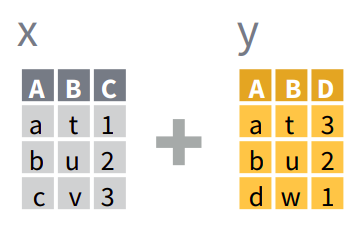
\includegraphics{img/join.png}

\begin{itemize}
\item
  \texttt{full\_join()}: devuelve todas las filas y todas las columnas de ambas tablas \texttt{x} e \texttt{y}.
  Cuando no coinciden los elementos en \texttt{x1}, devuelve \texttt{NA} (dato faltante).
  Esto significa que no se pierden filas de ninguna de las dos tablas aún cuando no hay coincidencia.
  Está es la manera más segura de unir tablas.
\item
  \texttt{left\_join()}: devuelve todas las filas de \texttt{x} y todas las columnas de \texttt{x} e \texttt{y}.
  Las filas en \texttt{x} que no tengan coincidencia con \texttt{y} tendrán \texttt{NA} en las nuevas columnas.
  Si hay múltiples coincidencias entre \texttt{x}e \texttt{y}, devuelve todas las coincidencias posibles.
\item
  \texttt{right\_join()}: es igual que \texttt{left\_join()} pero intercambiando el orden de \texttt{x} e \texttt{y}.
  En otras palabras, \texttt{right\_join(x,\ y)} es idéntico a \texttt{left\_join(y,\ x)}.
\item
  \texttt{inner\_join()}: devuelve todas las filas de \texttt{x} donde hay coincidencias con \texttt{y} y todas las columnas de \texttt{x} e \texttt{y}.
  Si hay múltiples coincidencias entre \texttt{x} e \texttt{y}, entonces devuelve todas las coincidencias.
  Esto significa que eliminará las filas (observaciones) que no coincidan en ambas tablas, lo que puede ser peligroso.
\end{itemize}

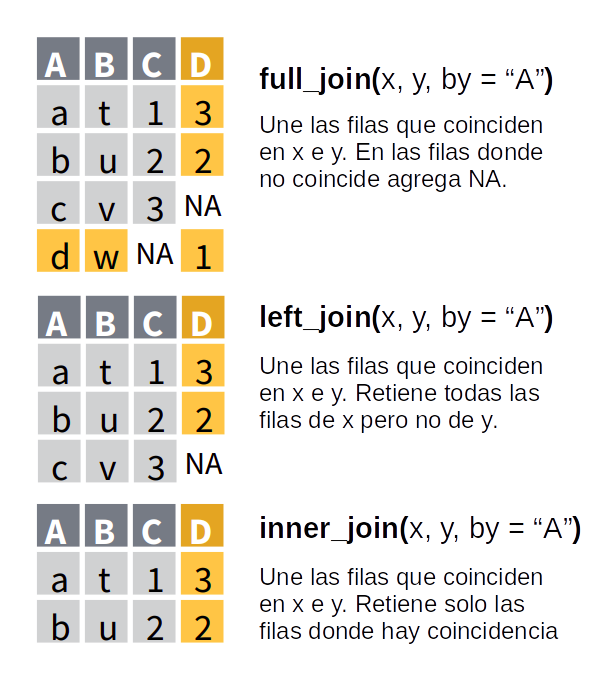
\includegraphics{img/join_family.png}

Ahora vamos a seguir trabajando con las base de datos de \texttt{paises} pero nos vamos a quedar solo con las observaciones del 2007 y de paso unirlo a una nueva base de datos \texttt{co2} que contiene información de la emisión de dióxido de carbono de cada país para ese mismo año.

\begin{Shaded}
\begin{Highlighting}[]
\NormalTok{paises\_2007 }\OtherTok{\textless{}{-}}\NormalTok{ readr}\SpecialCharTok{::}\FunctionTok{read\_csv}\NormalTok{(}\StringTok{"datos/paises.csv"}\NormalTok{) }\SpecialCharTok{\%\textgreater{}\%} 
  \FunctionTok{filter}\NormalTok{(anio }\SpecialCharTok{==} \DecValTok{2007}\NormalTok{) }

\NormalTok{co2\_2007 }\OtherTok{\textless{}{-}}\NormalTok{ readr}\SpecialCharTok{::}\FunctionTok{read\_csv}\NormalTok{(}\StringTok{"datos/co2\_2007.csv"}\NormalTok{)}
\NormalTok{co2\_2007}
\end{Highlighting}
\end{Shaded}

\begin{verbatim}
## # A tibble: 218 x 3
##    codigo_iso emision_co2 pais                  
##    <chr>            <dbl> <chr>                 
##  1 ABW            27.9    Aruba                 
##  2 AFG             0.0854 Afghanistán           
##  3 AGO             1.20   Angola                
##  4 ALB             1.32   Albania               
##  5 AND             6.52   Andorra               
##  6 ARB             4.10   Mundo Árabe           
##  7 ARE            22.4    Emiratos Árabes Unidos
##  8 ARG             4.38   Argentina             
##  9 ARM             1.73   Armenia               
## 10 ATG             5.14   Antigua y Barbuda     
## # ... with 208 more rows
\end{verbatim}

Esta nueva tabla tiene 3 columnas: \texttt{codigo\_iso} tiene el código ISO de 3 letras de (abreviaturas que se usan internacionalmente), \texttt{emision\_co2} tiene las emisiones anuales per cápita de CO2 en toneladas, \texttt{pais} tiene el nombre del país.
Esta última columna también está presente en la tabla \texttt{paises\_2007} y es la que va a servir como variable llave para unir las dos tablas.

Para unir las dos tablas, cualquier función \emph{join} requiere cierta información:

\begin{itemize}
\tightlist
\item
  las tablas a unir: son los dos primeros argumentos.
\item
  qué variable o variables (se puede usar más de una!) usar para identificar coincidencias: el argumento \texttt{by}.
\end{itemize}

Unamos \texttt{paises\_2007} y \texttt{co2\_2007} primero con \texttt{full\_join()}:

\begin{Shaded}
\begin{Highlighting}[]
\NormalTok{paises\_co2\_2007 }\OtherTok{\textless{}{-}} \FunctionTok{full\_join}\NormalTok{(paises\_2007, co2\_2007, }\AttributeTok{by =} \StringTok{"pais"}\NormalTok{)}
\NormalTok{paises\_co2\_2007}
\end{Highlighting}
\end{Shaded}

\begin{verbatim}
## # A tibble: 241 x 8
##    pais       continente  anio esperanza_de_vi~ poblacion pib_per_capita codigo_iso
##    <chr>      <chr>      <dbl>            <dbl>     <dbl>          <dbl> <chr>     
##  1 Afganistán Asia        2007             43.8  31889923           975. <NA>      
##  2 Albania    Europa      2007             76.4   3600523          5937. ALB       
##  3 Argelia    África      2007             72.3  33333216          6223. <NA>      
##  4 Angola     África      2007             42.7  12420476          4797. AGO       
##  5 Argentina  Américas    2007             75.3  40301927         12779. ARG       
##  6 Australia  Oceanía     2007             81.2  20434176         34435. AUS       
##  7 Austria    Europa      2007             79.8   8199783         36126. AUT       
##  8 Baréin     Asia        2007             75.6    708573         29796. <NA>      
##  9 Bangladesh Asia        2007             64.1 150448339          1391. BGD       
## 10 Bélgica    Europa      2007             79.4  10392226         33693. BEL       
## # ... with 231 more rows, and 1 more variable: emision_co2 <dbl>
\end{verbatim}

Si miramos de cerca la tabla unida veremos un par de cosas:

\begin{itemize}
\tightlist
\item
  Todas las columnas de \texttt{paises\_2007} y de \texttt{co2\_2007} están presentes.
\item
  Todas las observaciones están presentes, aún los países que están presentes en \texttt{co2\_2007} pero no en \texttt{paises\_2007} y viceversa. En esos casos ahora tenemos \texttt{NA}. Esto genera una tabla con 241 filas.
\end{itemize}

Esta es la opción más segura si no sabemos si todas las observaciones de una tabla están presente en a otra.

Si solo nos interesa conservar las filas de la tabla \emph{de la izquierda}, en este caso \texttt{paises\_2007} entonces:

\begin{Shaded}
\begin{Highlighting}[]
\NormalTok{paises\_co2\_2007 }\OtherTok{\textless{}{-}} \FunctionTok{left\_join}\NormalTok{(paises\_2007, co2\_2007, }\AttributeTok{by =} \StringTok{"pais"}\NormalTok{)}
\NormalTok{paises\_co2\_2007}
\end{Highlighting}
\end{Shaded}

\begin{verbatim}
## # A tibble: 142 x 8
##    pais       continente  anio esperanza_de_vi~ poblacion pib_per_capita codigo_iso
##    <chr>      <chr>      <dbl>            <dbl>     <dbl>          <dbl> <chr>     
##  1 Afganistán Asia        2007             43.8  31889923           975. <NA>      
##  2 Albania    Europa      2007             76.4   3600523          5937. ALB       
##  3 Argelia    África      2007             72.3  33333216          6223. <NA>      
##  4 Angola     África      2007             42.7  12420476          4797. AGO       
##  5 Argentina  Américas    2007             75.3  40301927         12779. ARG       
##  6 Australia  Oceanía     2007             81.2  20434176         34435. AUS       
##  7 Austria    Europa      2007             79.8   8199783         36126. AUT       
##  8 Baréin     Asia        2007             75.6    708573         29796. <NA>      
##  9 Bangladesh Asia        2007             64.1 150448339          1391. BGD       
## 10 Bélgica    Europa      2007             79.4  10392226         33693. BEL       
## # ... with 132 more rows, and 1 more variable: emision_co2 <dbl>
\end{verbatim}

Ahora esperamos que la tabla resultante tenga la misma cantidad de filas que \texttt{paises\_2007} y efectivamente eso ocurre.
Pero al mismo tiempo varios países en esa tabla no encontraron coincidencia en \texttt{co2\_2007} y por esa razón, la columna nueva columna \texttt{emisiones\_co2} tiene \texttt{NA}.

Finalmente, si quisiéramos quedarnos solo con las observaciones que están presentes en ambas tablas usamos \texttt{inner\_join()}.

\begin{Shaded}
\begin{Highlighting}[]
\NormalTok{paises\_co2\_2007 }\OtherTok{\textless{}{-}} \FunctionTok{inner\_join}\NormalTok{(paises\_2007, co2\_2007, }\AttributeTok{by =} \StringTok{"pais"}\NormalTok{)}
\NormalTok{paises\_co2\_2007}
\end{Highlighting}
\end{Shaded}

\begin{verbatim}
## # A tibble: 119 x 8
##    pais    continente  anio esperanza_de_vi~ poblacion pib_per_capita codigo_iso
##    <chr>   <chr>      <dbl>            <dbl>     <dbl>          <dbl> <chr>     
##  1 Albania Europa      2007             76.4   3600523          5937. ALB       
##  2 Angola  África      2007             42.7  12420476          4797. AGO       
##  3 Argent~ Américas    2007             75.3  40301927         12779. ARG       
##  4 Austra~ Oceanía     2007             81.2  20434176         34435. AUS       
##  5 Austria Europa      2007             79.8   8199783         36126. AUT       
##  6 Bangla~ Asia        2007             64.1 150448339          1391. BGD       
##  7 Bélgica Europa      2007             79.4  10392226         33693. BEL       
##  8 Bolivia Américas    2007             65.6   9119152          3822. BOL       
##  9 Bosnia~ Europa      2007             74.9   4552198          7446. BIH       
## 10 Botswa~ África      2007             50.7   1639131         12570. BWA       
## # ... with 109 more rows, and 1 more variable: emision_co2 <dbl>
\end{verbatim}

En este caso, perdemos las filas de \texttt{co2\_2007} que no encontraron coincidencia en \texttt{paises\_2007} y viceversa y la tabla resultante tiene aún menos filas (119).

\textbf{Desafío}

Estuvimos trabajando con una parte de la base de datos de emisiones.
Pero también está disponible \texttt{co2\_completo.csv} que contiene las emisiones para distintos años.
El objetivo es que unas \texttt{paises} y \texttt{co2} teniendo en cuenta tanto el país como el año.
Para eso:

\begin{enumerate}
\def\labelenumi{\arabic{enumi}.}
\tightlist
\item
  Lee la base de datos \texttt{co2\_completo.csv} en una nueva variable que se llame \texttt{co2}.
\item
  Revisá el nombre de las variables en esta base de datos, ¿se llaman igual que las variables en \texttt{paises}?
\item
  Uní las dos tablas usando \texttt{full\_join()}, tené en cuenta que ahora usamos dos variables llave \texttt{pais} y \texttt{anio}. Buscá en la documentación cómo indicarle eso a la función \texttt{full\_join()}.\\
\end{enumerate}

\hypertarget{manipulaciuxf3n-de-datos-ordenados-usando-dplyr-y-tidyr-ii-1}{%
\chapter{Manipulación de datos ordenados usando \{dplyr\} y \{tidyr\} II}\label{manipulaciuxf3n-de-datos-ordenados-usando-dplyr-y-tidyr-ii-1}}

En \href{04-lectura-datos.html\#Formatos_de_tablas}{la última sección de lectura de datos} viste el concepto de datos ``anchos'' y ``largos''.

Los datos en formato ``largo'' o ``tidy'', son aquellos en los cuales:

\begin{itemize}
\tightlist
\item
  cada fila es una observación
\item
  cada columna es una variable
\end{itemize}

En el formato ``ancho'' es un poco más complejo de definirlo pero la idea general es que:

\begin{itemize}
\tightlist
\item
  cada fila es un ``item''
\item
  cada columna es una variable
\end{itemize}

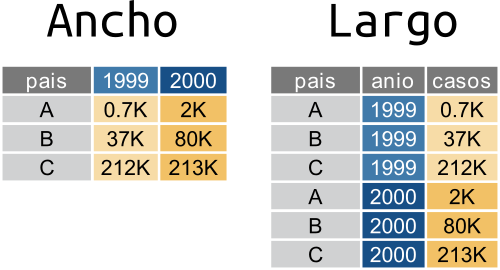
\includegraphics{img/largo-ancho.png}

Una tabla en formato largo va a tener una cierta cantidad de columnas que cumplen el rol de \emph{identificadores} y cuya combinación identifican una única observación y una única columna con el valor de la observación.
En el ejemplo de arriba, \texttt{pais} y \texttt{anio} son las columnas identificadoras y \texttt{casos} es la columna que contiene el valor de las observaciones.

En una tabla ancha, cada observación única se identifica a partir de la intersección de filas y columnas.
En el ejemplo, los países están en las filas y los años en las columnas.

En general, el formato ancho es más compacto y legible por humanos mientras que el largo es más fácil de manejar con la computadora.
Si te fijás en las tablas de arriba, es más fácil comparar los valores entre países y entre años en la tabla ancha.
Pero el nombre de las columnas (``1999'', ``2000'') en realidad ¡son datos!
Además este formato se empieza a complicar en cuanto hay más de dos identificadores.

Un mismo set de datos puede ser representado de forma completamente ``larga'', completamente ``ancha'' o --lo que es más común-- en un formato intermedio pero no existe una forma ``correcta'' de organizar los datos; cada una tiene sus ventajas y desventajas.
Por esto es que es muy normal que durante un análisis los datos vayan y vuelvan entre distintos formatos dependiendo de los métodos estadísticos que se le aplican.
Entonces, aprender a transformar datos anchos en largos y viceversa es un habilidad muy útil.

\textbf{Desafío}

En las tablas de ejemplo cada país tiene el un valor observado de ``casos'' para cada año.
¿Cómo agregarías una nueva variable con información sobre ``precios''?
Dibujá un esquema en papel y lápiz en formato ancho y uno en formato largo.
¿En qué formato es más ``natural'' esa extensión?

En esta sección vas a usar el paquete \{tidyr\} para manipular datos.
Si no lo tenés instalado, instalalo con el comando:

\begin{Shaded}
\begin{Highlighting}[]
\FunctionTok{install.packages}\NormalTok{(}\StringTok{"tidyr"}\NormalTok{)}
\end{Highlighting}
\end{Shaded}

(como siempre, recordá que esto hay que hacerlo una única vez)

Y luego cargá \{tidyr\} y \{dplyr\} (que usaste en \href{05-dplyr-I.html}{una sección anterior}) con:

\begin{Shaded}
\begin{Highlighting}[]
\FunctionTok{library}\NormalTok{(tidyr)}
\FunctionTok{library}\NormalTok{(dplyr)}
\end{Highlighting}
\end{Shaded}

\hypertarget{de-ancho-a-largo-con-pivot_longer-1}{%
\section{\texorpdfstring{De ancho a largo con \texttt{pivot\_longer()}}{De ancho a largo con pivot\_longer()}}\label{de-ancho-a-largo-con-pivot_longer-1}}

En secciones anteriores usaste una versión de los datos de \href{https://www.gapminder.org/}{gapminder}.
Ahora vas a leer los datos en su formato original:

\begin{Shaded}
\begin{Highlighting}[]
\NormalTok{paises\_ancho }\OtherTok{\textless{}{-}}\NormalTok{ readr}\SpecialCharTok{::}\FunctionTok{read\_csv}\NormalTok{(}\StringTok{"datos/paises\_ancho.csv"}\NormalTok{)}
\end{Highlighting}
\end{Shaded}

\begin{verbatim}
## Rows: 142 Columns: 38
\end{verbatim}

\begin{verbatim}
## -- Column specification --------------------------------------------------------
## Delimiter: ","
## chr  (2): continente, pais
## dbl (36): pib_per_capita_1952, pib_per_capita_1957, pib_per_capita_1962, pib...
\end{verbatim}

\begin{verbatim}
## 
## i Use `spec()` to retrieve the full column specification for this data.
## i Specify the column types or set `show_col_types = FALSE` to quiet this message.
\end{verbatim}

\begin{Shaded}
\begin{Highlighting}[]
\NormalTok{paises\_ancho}
\end{Highlighting}
\end{Shaded}

\begin{verbatim}
## # A tibble: 142 x 38
##    continente pais                     pib_per_capita_~ pib_per_capita_~ pib_per_capita_~
##    <chr>      <chr>                               <dbl>            <dbl>            <dbl>
##  1 Africa     Algeria                             2449.            3014.            2551.
##  2 Africa     Angola                              3521.            3828.            4269.
##  3 Africa     Benin                               1063.             960.             949.
##  4 Africa     Botswana                             851.             918.             984.
##  5 Africa     Burkina Faso                         543.             617.             723.
##  6 Africa     Burundi                              339.             380.             355.
##  7 Africa     Cameroon                            1173.            1313.            1400.
##  8 Africa     Central African Republic            1071.            1191.            1193.
##  9 Africa     Chad                                1179.            1308.            1390.
## 10 Africa     Comoros                             1103.            1211.            1407.
## # ... with 132 more rows, and 33 more variables: pib_per_capita_1967 <dbl>,
## #   pib_per_capita_1972 <dbl>, pib_per_capita_1977 <dbl>,
## #   pib_per_capita_1982 <dbl>, pib_per_capita_1987 <dbl>,
## #   pib_per_capita_1992 <dbl>, pib_per_capita_1997 <dbl>,
## #   pib_per_capita_2002 <dbl>, pib_per_capita_2007 <dbl>,
## #   esperanza_de_vida_1952 <dbl>, esperanza_de_vida_1957 <dbl>,
## #   esperanza_de_vida_1962 <dbl>, esperanza_de_vida_1967 <dbl>, ...
\end{verbatim}

¿Notaste que en el código anterior no usaste \texttt{library(readr)} para cargar el paquete y luego leer?
Con la notación \texttt{paquete::funcion()} podés acceder a las funciones de un paquete sin tener que cargarlo.
Es una buena forma de no tener que cargar un montón de paquetes innecesarios si vas a correr una única función de un paquete pocas veces.

Esta tabla, increíblemente ancha, es muy difícil de manejar.
Por ejemplo, es imposible hacer una serie de tiempo de una variable, o calcular el promedio por variable y país; ni hablar de calcular una regresión lineal.

Para convertirlo en una tabla más larga, se usa \texttt{pivot\_longer()} (``longer'' es ``más largo'' en inglés):

\begin{Shaded}
\begin{Highlighting}[]
\NormalTok{paises\_largo }\OtherTok{\textless{}{-}} \FunctionTok{pivot\_longer}\NormalTok{(paises\_ancho,}
                             \AttributeTok{cols =} \FunctionTok{c}\NormalTok{(}\FunctionTok{starts\_with}\NormalTok{(}\StringTok{\textquotesingle{}pob\textquotesingle{}}\NormalTok{), }
                                      \FunctionTok{starts\_with}\NormalTok{(}\StringTok{\textquotesingle{}esperanza\textquotesingle{}}\NormalTok{), }
                                      \FunctionTok{starts\_with}\NormalTok{(}\StringTok{\textquotesingle{}pib\_per\textquotesingle{}}\NormalTok{)),}
                             \AttributeTok{names\_to =} \StringTok{"variable\_anio"}\NormalTok{, }
                             \AttributeTok{values\_to =} \StringTok{"valor"}
\NormalTok{)}
\NormalTok{paises\_largo}
\end{Highlighting}
\end{Shaded}

\begin{verbatim}
## # A tibble: 5,112 x 4
##    continente pais    variable_anio     valor
##    <chr>      <chr>   <chr>             <dbl>
##  1 Africa     Algeria poblacion_1952  9279525
##  2 Africa     Algeria poblacion_1957 10270856
##  3 Africa     Algeria poblacion_1962 11000948
##  4 Africa     Algeria poblacion_1967 12760499
##  5 Africa     Algeria poblacion_1972 14760787
##  6 Africa     Algeria poblacion_1977 17152804
##  7 Africa     Algeria poblacion_1982 20033753
##  8 Africa     Algeria poblacion_1987 23254956
##  9 Africa     Algeria poblacion_1992 26298373
## 10 Africa     Algeria poblacion_1997 29072015
## # ... with 5,102 more rows
\end{verbatim}

El primer argumento de\texttt{pivot\_longer()} es la tabla que va a modificar: \texttt{paises\_ancho}.
El segundo argumento se llama \texttt{cols} y es un vector con las columnas que tienen los valores a ``alargar''.
Podría ser un vector escrito a mano (algo como \texttt{c("pib\_per\_capita\_1952",\ "pib\_per\_capita\_1957"...)}) pero con más de 30 columnas, escribir todo eso sería tedioso y probablemente estaría lleno de errores.
Por eso \{tidyr\} provee funciones de ayuda para seleccionar columnas en base a patrones.
El código de arriba usa \texttt{starts\_with()} que, como su nombre en inglés lo indica, selecciona las columnas que \emph{empiezan con} una determinada cadena de caracteres.
El vector \texttt{c(starts\_with(\textquotesingle{}pob\textquotesingle{}),\ starts\_with(\textquotesingle{}esperanza\textquotesingle{}),\ starts\_with(\textquotesingle{}pib\_per\textquotesingle{}))} le dice a \texttt{pivot\_longer()} que seleccione las columnas que empieza con ``pob'', las que empiezan con ``esperanza'' y las que empiezan con ``pib\_per''.

Estas funciones accesorias para seleccionar muchas funciones se llaman ``tidyselect''.
Si querés leer más detalles de las distintas formas que podés seleccionar variables leé la documentación usando \texttt{?tidyselect::language}.

El tercer y cuarto argumento son los nombres de las columnas de ``nombre'' y de ``valor'' que va a tener la nueva tabla.
Como la nueva columna de identificación tiene los datos de la variable y el año a medir, ``variable\_anio'' es un buen nombre.
Y la columna de valor va a tener\ldots{} bueno, el valor.

Tomate un momento para visualizar lo que acaba de pasar.
La tabla ancha tenía un montón de columnas con distintos datos.
Ahora estos datos están uno arriba de otro en la columna ``valor'', pero para identificar el nombre de la columna de la cual vinieron, se agrega la columna ``variable\_anio''.

\begin{figure}
\centering
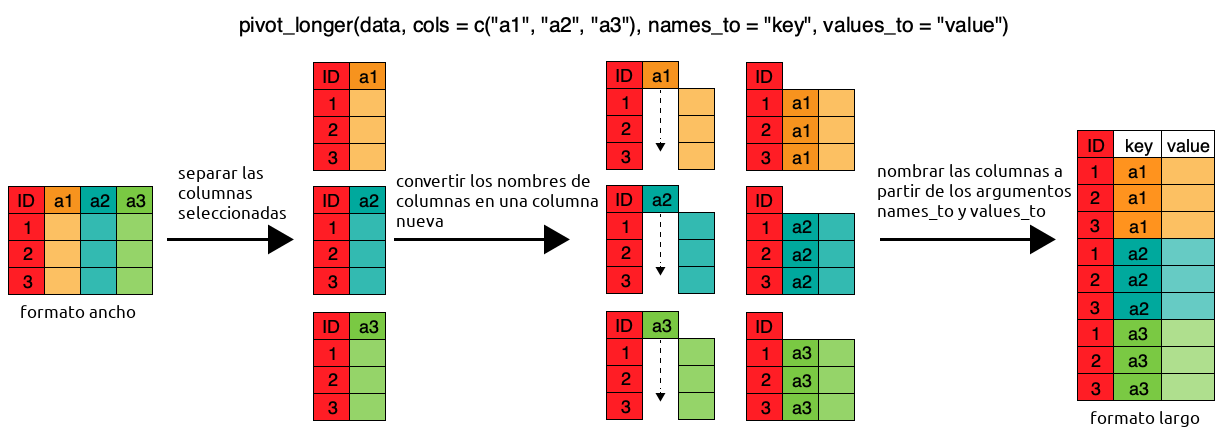
\includegraphics{img/ancho-a-largo.png}
\caption{Proceso de largo a ancho}
\end{figure}

La columna \texttt{variable\_anio} todavía no es muy útil porque contiene 2 datos, la variable (población, expectativa de vida o PBI per cápita) y el año.
Sería mejor separar esta información en dos columnas llamadas ``variable'' y ``anio''.
Para eso está la función \texttt{separate()}.

\begin{Shaded}
\begin{Highlighting}[]
\FunctionTok{separate}\NormalTok{(paises\_largo, }
         \AttributeTok{col =}\NormalTok{ variable\_anio, }
         \AttributeTok{into =} \FunctionTok{c}\NormalTok{(}\StringTok{"variable"}\NormalTok{, }\StringTok{"anio"}\NormalTok{), }
         \AttributeTok{sep =} \SpecialCharTok{{-}}\DecValTok{4}\NormalTok{)}
\end{Highlighting}
\end{Shaded}

\begin{verbatim}
## # A tibble: 5,112 x 5
##    continente pais    variable   anio     valor
##    <chr>      <chr>   <chr>      <chr>    <dbl>
##  1 Africa     Algeria poblacion_ 1952   9279525
##  2 Africa     Algeria poblacion_ 1957  10270856
##  3 Africa     Algeria poblacion_ 1962  11000948
##  4 Africa     Algeria poblacion_ 1967  12760499
##  5 Africa     Algeria poblacion_ 1972  14760787
##  6 Africa     Algeria poblacion_ 1977  17152804
##  7 Africa     Algeria poblacion_ 1982  20033753
##  8 Africa     Algeria poblacion_ 1987  23254956
##  9 Africa     Algeria poblacion_ 1992  26298373
## 10 Africa     Algeria poblacion_ 1997  29072015
## # ... with 5,102 more rows
\end{verbatim}

El primer argumento, como siempre, es la tabla a procesar.
El segundo, \texttt{col}, es la columna a separar en dos (o más) columnas nuevas.
El tercero, \texttt{into} es el nombre de las nuevas columnas que \texttt{separate()} va a crear.
El último argumento es \texttt{sep} que define cómo realizar la separación.
Por defecto, \texttt{sep} es una \href{https://es.wikipedia.org/wiki/Expresi\%C3\%B3n_regular}{expresión regular} que captura cualquier caracter no alfanumérico.
En el caso de \texttt{variable\_anio} no sirve, porque para valores como \texttt{"esperanza\_de\_vida\_1952"}, separaría en \texttt{"esperanza"}, \texttt{"de"}, \texttt{"vida"} y \texttt{"1952"}.
Como el año tiene siempre 4 caracteres, una solución simple es usar \texttt{sep\ =\ -4}, que significa que la separación es 4 caracteres contando desde el final.

Habrás notado un problema.
El texto en la columnas \texttt{variable} todavía tiene un ``\_'' al final.
Podrías usar \texttt{mutate()} y un poco de funciones de manipulación de caracteres para quitarlo, pero hay una forma un poco más simple y es separando la columna \texttt{variable\_anio} en tres, incluyendo una columna con el guión:

\begin{Shaded}
\begin{Highlighting}[]
\NormalTok{paises\_largo }\OtherTok{\textless{}{-}} \FunctionTok{separate}\NormalTok{(paises\_largo, }
         \AttributeTok{col =}\NormalTok{ variable\_anio, }
         \AttributeTok{into =} \FunctionTok{c}\NormalTok{(}\StringTok{"variable"}\NormalTok{, }\StringTok{"guion"}\NormalTok{, }\StringTok{"anio"}\NormalTok{), }
         \AttributeTok{sep =} \FunctionTok{c}\NormalTok{(}\SpecialCharTok{{-}}\DecValTok{5}\NormalTok{, }\SpecialCharTok{{-}}\DecValTok{4}\NormalTok{))}
\NormalTok{paises\_largo}
\end{Highlighting}
\end{Shaded}

\begin{verbatim}
## # A tibble: 5,112 x 6
##    continente pais    variable  guion anio     valor
##    <chr>      <chr>   <chr>     <chr> <chr>    <dbl>
##  1 Africa     Algeria poblacion _     1952   9279525
##  2 Africa     Algeria poblacion _     1957  10270856
##  3 Africa     Algeria poblacion _     1962  11000948
##  4 Africa     Algeria poblacion _     1967  12760499
##  5 Africa     Algeria poblacion _     1972  14760787
##  6 Africa     Algeria poblacion _     1977  17152804
##  7 Africa     Algeria poblacion _     1982  20033753
##  8 Africa     Algeria poblacion _     1987  23254956
##  9 Africa     Algeria poblacion _     1992  26298373
## 10 Africa     Algeria poblacion _     1997  29072015
## # ... with 5,102 more rows
\end{verbatim}

Y ya casi.
Hay que eliminar la columna \texttt{guion}, que no sirve para nada.
Pero fijate que debajo de la columna \texttt{anio} dice \texttt{\textless{}chr\textgreater{}}; eso significa que el tipo de la columna es caracter, pero los años son números.
Usando \texttt{mutate()} podés eliminar la columna \texttt{guion} asignándole el valor \texttt{NULL} (nulo) y coercer (recordá \href{04-lectura-datos.html\#Vectores}{esta sección}) la columna \texttt{anio} a entero usando \texttt{as.integer()}:

\begin{Shaded}
\begin{Highlighting}[]
\NormalTok{paises\_largo }\OtherTok{\textless{}{-}} \FunctionTok{mutate}\NormalTok{(paises\_largo, }
                       \AttributeTok{guion =} \ConstantTok{NULL}\NormalTok{,}
                       \AttributeTok{anio =} \FunctionTok{as.integer}\NormalTok{(anio))}
\NormalTok{paises\_largo}
\end{Highlighting}
\end{Shaded}

\begin{verbatim}
## # A tibble: 5,112 x 5
##    continente pais    variable   anio    valor
##    <chr>      <chr>   <chr>     <int>    <dbl>
##  1 Africa     Algeria poblacion  1952  9279525
##  2 Africa     Algeria poblacion  1957 10270856
##  3 Africa     Algeria poblacion  1962 11000948
##  4 Africa     Algeria poblacion  1967 12760499
##  5 Africa     Algeria poblacion  1972 14760787
##  6 Africa     Algeria poblacion  1977 17152804
##  7 Africa     Algeria poblacion  1982 20033753
##  8 Africa     Algeria poblacion  1987 23254956
##  9 Africa     Algeria poblacion  1992 26298373
## 10 Africa     Algeria poblacion  1997 29072015
## # ... with 5,102 more rows
\end{verbatim}

\textbf{Desafío}

Juntá todos los pasos anteriores en una sola cadena de operaciones usando \texttt{\%\textgreater{}\%}.

\hypertarget{de-largo-a-ancho-con-pivot_wider-1}{%
\section{\texorpdfstring{De largo a ancho con \texttt{pivot\_wider()}}{De largo a ancho con pivot\_wider()}}\label{de-largo-a-ancho-con-pivot_wider-1}}

Ahora la variable \texttt{paises\_largo} está en el formato más largo posible.
Tiene 5 columnas, de las cuales sólo una es la columnas con valores.
Pero con los datos así no podrías hacer un gráfico de puntos que muestre la relación entre el PBI per cápita y la expectativa de vida como en la \href{06-graficos-I.html\#Segunda_capa:_geometrías}{sección de gráficos}.
Fijate que los valores de la columna \texttt{valor} no tienen todos las mismas unidades, por lo que operar con ese vector podría dar resultados sin sentido.
Muchas veces es conveniente y natural tener los datos en un formato intermedio en donde hay múltiples columnas con los valores de distintas variables observadas.

Pasa ``ensanchar'' una tabla está la función \texttt{pivot\_wider()} (``wider'' es ``más ancha'' en inglés) y el código para conseguir este formato intermedio es:

\begin{Shaded}
\begin{Highlighting}[]
\NormalTok{paises\_medio }\OtherTok{\textless{}{-}} \FunctionTok{pivot\_wider}\NormalTok{(paises\_largo, }\AttributeTok{names\_from =}\NormalTok{ variable, }\AttributeTok{values\_from =}\NormalTok{ valor)}
\NormalTok{paises\_medio}
\end{Highlighting}
\end{Shaded}

\begin{verbatim}
## # A tibble: 1,704 x 6
##    continente pais     anio poblacion esperanza_de_vida pib_per_capita
##    <chr>      <chr>   <int>     <dbl>             <dbl>          <dbl>
##  1 Africa     Algeria  1952   9279525              43.1          2449.
##  2 Africa     Algeria  1957  10270856              45.7          3014.
##  3 Africa     Algeria  1962  11000948              48.3          2551.
##  4 Africa     Algeria  1967  12760499              51.4          3247.
##  5 Africa     Algeria  1972  14760787              54.5          4183.
##  6 Africa     Algeria  1977  17152804              58.0          4910.
##  7 Africa     Algeria  1982  20033753              61.4          5745.
##  8 Africa     Algeria  1987  23254956              65.8          5681.
##  9 Africa     Algeria  1992  26298373              67.7          5023.
## 10 Africa     Algeria  1997  29072015              69.2          4797.
## # ... with 1,694 more rows
\end{verbatim}

Nuevamente el primer argumento es la tabla original.
El segundo, \texttt{names\_from} es la columna cuyos valores únicos van a convertirse en nuevas columnas.
La columna \texttt{variable} tiene los valores \texttt{"población"}, \texttt{"esperanza\_de\_vida"} y \texttt{"pib\_per\_capita"} y entonces la tabla nueva tendrá tres columnas con esos nombres.
El tercer argumento, \texttt{values\_from}, es la columna de la cual sacar los valores.

Para volver al formato más ancho, basta con agregar más columnas en el argumento \texttt{names\_from}:

\begin{Shaded}
\begin{Highlighting}[]
\FunctionTok{pivot\_wider}\NormalTok{(paises\_largo, }
            \AttributeTok{names\_from =} \FunctionTok{c}\NormalTok{(variable, anio), }
            \AttributeTok{names\_sep =} \StringTok{"\_"}\NormalTok{,}
            \AttributeTok{values\_from =}\NormalTok{ valor)}
\end{Highlighting}
\end{Shaded}

\begin{verbatim}
## # A tibble: 142 x 38
##    continente pais   poblacion_1952 poblacion_1957 poblacion_1962 poblacion_1967
##    <chr>      <chr>           <dbl>          <dbl>          <dbl>          <dbl>
##  1 Africa     Alger~        9279525       10270856       11000948       12760499
##  2 Africa     Angola        4232095        4561361        4826015        5247469
##  3 Africa     Benin         1738315        1925173        2151895        2427334
##  4 Africa     Botsw~         442308         474639         512764         553541
##  5 Africa     Burki~        4469979        4713416        4919632        5127935
##  6 Africa     Burun~        2445618        2667518        2961915        3330989
##  7 Africa     Camer~        5009067        5359923        5793633        6335506
##  8 Africa     Centr~        1291695        1392284        1523478        1733638
##  9 Africa     Chad          2682462        2894855        3150417        3495967
## 10 Africa     Comor~         153936         170928         191689         217378
## # ... with 132 more rows, and 32 more variables: poblacion_1972 <dbl>,
## #   poblacion_1977 <dbl>, poblacion_1982 <dbl>, poblacion_1987 <dbl>,
## #   poblacion_1992 <dbl>, poblacion_1997 <dbl>, poblacion_2002 <dbl>,
## #   poblacion_2007 <dbl>, esperanza_de_vida_1952 <dbl>,
## #   esperanza_de_vida_1957 <dbl>, esperanza_de_vida_1962 <dbl>,
## #   esperanza_de_vida_1967 <dbl>, esperanza_de_vida_1972 <dbl>,
## #   esperanza_de_vida_1977 <dbl>, esperanza_de_vida_1982 <dbl>, ...
\end{verbatim}

En esta llamada también está el argumento \texttt{names\_sep}, que determina el caracter que se usa para crear el nombre de las nuevas columnas.

\textbf{Desafío}

\begin{itemize}
\item
  Creá una nueva tabla, llamada \texttt{paises\_superduper\_ancho} que tenga una columna para cada variable, anio y país.
  (Consejo: la tabla final tiene que tener 5 filas).
\item
  ¿Cómo es la tabla más ancha posible que podés generar con estos datos?
  ¿Cuántas filas y columnas tiene?
\end{itemize}

\hypertarget{uniendo-tablas-1}{%
\section{Uniendo tablas}\label{uniendo-tablas-1}}

Hasta ahora todo lo que usaste de \{dplyr\} involucra trabajar y modificar con una sola tabla a la vez, pero es muy común tener dos o más tablas con datos relacionados.
En ese caso, tenemos que \emph{unir} estas tablas.
a partir de una o más variables en común o \emph{keys}.
En Excel u otro programa de hojas de cálculo, esto se resuelve con la función ``VLOOKUP'' o ``BUSCARV'', en R y en particular dentro del mundo de \{dplyr\} hay que usar la familia de funciones \texttt{*\_join()}.
Hay una función cada tipo de unión que queramos hacer.

Asumiendo que querés unir dos data.frames o tablas \texttt{x} e \texttt{y} que tienen en común una variable \texttt{A}:

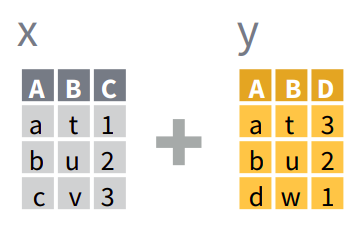
\includegraphics{img/join.png}

\begin{itemize}
\item
  \texttt{full\_join()}: devuelve todas las filas y todas las columnas de ambas tablas \texttt{x} e \texttt{y}.
  Cuando no coinciden los elementos en \texttt{x1}, devuelve \texttt{NA} (dato faltante).
  Esto significa que no se pierden filas de ninguna de las dos tablas aún cuando no hay coincidencia.
  Está es la manera más segura de unir tablas.
\item
  \texttt{left\_join()}: devuelve todas las filas de \texttt{x} y todas las columnas de \texttt{x} e \texttt{y}.
  Las filas en \texttt{x} que no tengan coincidencia con \texttt{y} tendrán \texttt{NA} en las nuevas columnas.
  Si hay múltiples coincidencias entre \texttt{x}e \texttt{y}, devuelve todas las coincidencias posibles.
\item
  \texttt{right\_join()}: es igual que \texttt{left\_join()} pero intercambiando el orden de \texttt{x} e \texttt{y}.
  En otras palabras, \texttt{right\_join(x,\ y)} es idéntico a \texttt{left\_join(y,\ x)}.
\item
  \texttt{inner\_join()}: devuelve todas las filas de \texttt{x} donde hay coincidencias con \texttt{y} y todas las columnas de \texttt{x} e \texttt{y}.
  Si hay múltiples coincidencias entre \texttt{x} e \texttt{y}, entonces devuelve todas las coincidencias.
  Esto significa que eliminará las filas (observaciones) que no coincidan en ambas tablas, lo que puede ser peligroso.
\end{itemize}

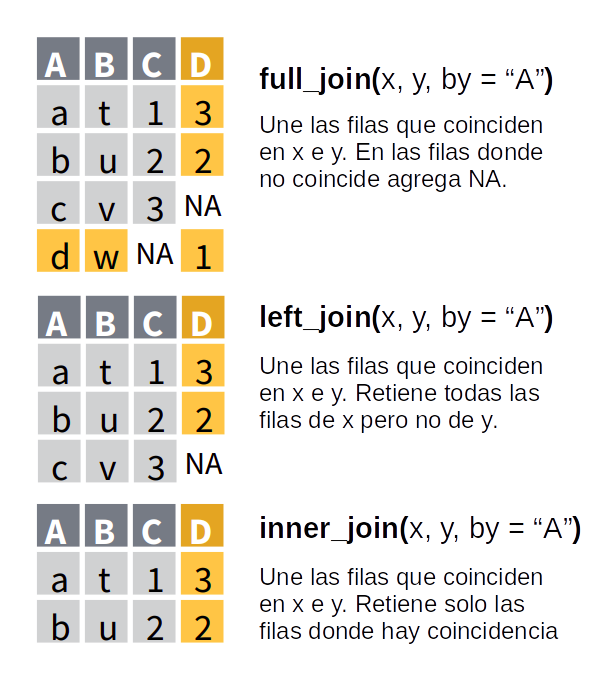
\includegraphics{img/join_family.png}

Ahora vamos a seguir trabajando con las base de datos de \texttt{paises} pero nos vamos a quedar solo con las observaciones del 2007 y de paso unirlo a una nueva base de datos \texttt{co2} que contiene información de la emisión de dióxido de carbono de cada país para ese mismo año.

\begin{Shaded}
\begin{Highlighting}[]
\NormalTok{paises\_2007 }\OtherTok{\textless{}{-}}\NormalTok{ readr}\SpecialCharTok{::}\FunctionTok{read\_csv}\NormalTok{(}\StringTok{"datos/paises.csv"}\NormalTok{) }\SpecialCharTok{\%\textgreater{}\%} 
  \FunctionTok{filter}\NormalTok{(anio }\SpecialCharTok{==} \DecValTok{2007}\NormalTok{) }

\NormalTok{co2\_2007 }\OtherTok{\textless{}{-}}\NormalTok{ readr}\SpecialCharTok{::}\FunctionTok{read\_csv}\NormalTok{(}\StringTok{"datos/co2\_2007.csv"}\NormalTok{)}
\NormalTok{co2\_2007}
\end{Highlighting}
\end{Shaded}

\begin{verbatim}
## # A tibble: 218 x 3
##    codigo_iso emision_co2 pais                  
##    <chr>            <dbl> <chr>                 
##  1 ABW            27.9    Aruba                 
##  2 AFG             0.0854 Afghanistán           
##  3 AGO             1.20   Angola                
##  4 ALB             1.32   Albania               
##  5 AND             6.52   Andorra               
##  6 ARB             4.10   Mundo Árabe           
##  7 ARE            22.4    Emiratos Árabes Unidos
##  8 ARG             4.38   Argentina             
##  9 ARM             1.73   Armenia               
## 10 ATG             5.14   Antigua y Barbuda     
## # ... with 208 more rows
\end{verbatim}

Esta nueva tabla tiene 3 columnas: \texttt{codigo\_iso} tiene el código ISO de 3 letras de (abreviaturas que se usan internacionalmente), \texttt{emision\_co2} tiene las emisiones anuales per cápita de CO2 en toneladas, \texttt{pais} tiene el nombre del país.
Esta última columna también está presente en la tabla \texttt{paises\_2007} y es la que va a servir como variable llave para unir las dos tablas.

Para unir las dos tablas, cualquier función \emph{join} requiere cierta información:

\begin{itemize}
\tightlist
\item
  las tablas a unir: son los dos primeros argumentos.
\item
  qué variable o variables (se puede usar más de una!) usar para identificar coincidencias: el argumento \texttt{by}.
\end{itemize}

Unamos \texttt{paises\_2007} y \texttt{co2\_2007} primero con \texttt{full\_join()}:

\begin{Shaded}
\begin{Highlighting}[]
\NormalTok{paises\_co2\_2007 }\OtherTok{\textless{}{-}} \FunctionTok{full\_join}\NormalTok{(paises\_2007, co2\_2007, }\AttributeTok{by =} \StringTok{"pais"}\NormalTok{)}
\NormalTok{paises\_co2\_2007}
\end{Highlighting}
\end{Shaded}

\begin{verbatim}
## # A tibble: 241 x 8
##    pais       continente  anio esperanza_de_vi~ poblacion pib_per_capita codigo_iso
##    <chr>      <chr>      <dbl>            <dbl>     <dbl>          <dbl> <chr>     
##  1 Afganistán Asia        2007             43.8  31889923           975. <NA>      
##  2 Albania    Europa      2007             76.4   3600523          5937. ALB       
##  3 Argelia    África      2007             72.3  33333216          6223. <NA>      
##  4 Angola     África      2007             42.7  12420476          4797. AGO       
##  5 Argentina  Américas    2007             75.3  40301927         12779. ARG       
##  6 Australia  Oceanía     2007             81.2  20434176         34435. AUS       
##  7 Austria    Europa      2007             79.8   8199783         36126. AUT       
##  8 Baréin     Asia        2007             75.6    708573         29796. <NA>      
##  9 Bangladesh Asia        2007             64.1 150448339          1391. BGD       
## 10 Bélgica    Europa      2007             79.4  10392226         33693. BEL       
## # ... with 231 more rows, and 1 more variable: emision_co2 <dbl>
\end{verbatim}

Si miramos de cerca la tabla unida veremos un par de cosas:

\begin{itemize}
\tightlist
\item
  Todas las columnas de \texttt{paises\_2007} y de \texttt{co2\_2007} están presentes.
\item
  Todas las observaciones están presentes, aún los países que están presentes en \texttt{co2\_2007} pero no en \texttt{paises\_2007} y viceversa. En esos casos ahora tenemos \texttt{NA}. Esto genera una tabla con 241 filas.
\end{itemize}

Esta es la opción más segura si no sabemos si todas las observaciones de una tabla están presente en a otra.

Si solo nos interesa conservar las filas de la tabla \emph{de la izquierda}, en este caso \texttt{paises\_2007} entonces:

\begin{Shaded}
\begin{Highlighting}[]
\NormalTok{paises\_co2\_2007 }\OtherTok{\textless{}{-}} \FunctionTok{left\_join}\NormalTok{(paises\_2007, co2\_2007, }\AttributeTok{by =} \StringTok{"pais"}\NormalTok{)}
\NormalTok{paises\_co2\_2007}
\end{Highlighting}
\end{Shaded}

\begin{verbatim}
## # A tibble: 142 x 8
##    pais       continente  anio esperanza_de_vi~ poblacion pib_per_capita codigo_iso
##    <chr>      <chr>      <dbl>            <dbl>     <dbl>          <dbl> <chr>     
##  1 Afganistán Asia        2007             43.8  31889923           975. <NA>      
##  2 Albania    Europa      2007             76.4   3600523          5937. ALB       
##  3 Argelia    África      2007             72.3  33333216          6223. <NA>      
##  4 Angola     África      2007             42.7  12420476          4797. AGO       
##  5 Argentina  Américas    2007             75.3  40301927         12779. ARG       
##  6 Australia  Oceanía     2007             81.2  20434176         34435. AUS       
##  7 Austria    Europa      2007             79.8   8199783         36126. AUT       
##  8 Baréin     Asia        2007             75.6    708573         29796. <NA>      
##  9 Bangladesh Asia        2007             64.1 150448339          1391. BGD       
## 10 Bélgica    Europa      2007             79.4  10392226         33693. BEL       
## # ... with 132 more rows, and 1 more variable: emision_co2 <dbl>
\end{verbatim}

Ahora esperamos que la tabla resultante tenga la misma cantidad de filas que \texttt{paises\_2007} y efectivamente eso ocurre.
Pero al mismo tiempo varios países en esa tabla no encontraron coincidencia en \texttt{co2\_2007} y por esa razón, la columna nueva columna \texttt{emisiones\_co2} tiene \texttt{NA}.

Finalmente, si quisiéramos quedarnos solo con las observaciones que están presentes en ambas tablas usamos \texttt{inner\_join()}.

\begin{Shaded}
\begin{Highlighting}[]
\NormalTok{paises\_co2\_2007 }\OtherTok{\textless{}{-}} \FunctionTok{inner\_join}\NormalTok{(paises\_2007, co2\_2007, }\AttributeTok{by =} \StringTok{"pais"}\NormalTok{)}
\NormalTok{paises\_co2\_2007}
\end{Highlighting}
\end{Shaded}

\begin{verbatim}
## # A tibble: 119 x 8
##    pais    continente  anio esperanza_de_vi~ poblacion pib_per_capita codigo_iso
##    <chr>   <chr>      <dbl>            <dbl>     <dbl>          <dbl> <chr>     
##  1 Albania Europa      2007             76.4   3600523          5937. ALB       
##  2 Angola  África      2007             42.7  12420476          4797. AGO       
##  3 Argent~ Américas    2007             75.3  40301927         12779. ARG       
##  4 Austra~ Oceanía     2007             81.2  20434176         34435. AUS       
##  5 Austria Europa      2007             79.8   8199783         36126. AUT       
##  6 Bangla~ Asia        2007             64.1 150448339          1391. BGD       
##  7 Bélgica Europa      2007             79.4  10392226         33693. BEL       
##  8 Bolivia Américas    2007             65.6   9119152          3822. BOL       
##  9 Bosnia~ Europa      2007             74.9   4552198          7446. BIH       
## 10 Botswa~ África      2007             50.7   1639131         12570. BWA       
## # ... with 109 more rows, and 1 more variable: emision_co2 <dbl>
\end{verbatim}

En este caso, perdemos las filas de \texttt{co2\_2007} que no encontraron coincidencia en \texttt{paises\_2007} y viceversa y la tabla resultante tiene aún menos filas (119).

\textbf{Desafío}

Estuvimos trabajando con una parte de la base de datos de emisiones.
Pero también está disponible \texttt{co2\_completo.csv} que contiene las emisiones para distintos años.
El objetivo es que unas \texttt{paises} y \texttt{co2} teniendo en cuenta tanto el país como el año.
Para eso:

\begin{enumerate}
\def\labelenumi{\arabic{enumi}.}
\tightlist
\item
  Lee la base de datos \texttt{co2\_completo.csv} en una nueva variable que se llame \texttt{co2}.
\item
  Revisá el nombre de las variables en esta base de datos, ¿se llaman igual que las variables en \texttt{paises}?
\item
  Uní las dos tablas usando \texttt{full\_join()}, tené en cuenta que ahora usamos dos variables llave \texttt{pais} y \texttt{anio}. Buscá en la documentación cómo indicarle eso a la función \texttt{full\_join()}.\\
\end{enumerate}

\hypertarget{reportes-ii}{%
\chapter{Reportes II}\label{reportes-ii}}

Durante este curso fuiste creando varios documentos con R Markdown en HTML. Este es un formato que tiene un montón de flexibilidad, pero seguramente no es el único que necesitás. Casi seguro que los informes los tengas que presentar en formato PDF o, incluso, ¡en papel impreso! \{Rmarkdown\}, y todo un amplio ecosistema de otros paquetes, permite generar documentos en múltiples formatos usando el mismo archivo de texto plano.

\hypertarget{eligiendo-el-formato-de-salida}{%
\section{Eligiendo el formato de salida}\label{eligiendo-el-formato-de-salida}}

Ya habrás visto esto cuando creás un archivo markdown nuevo, RStudio te permite elegir entre tres formatos de salida:

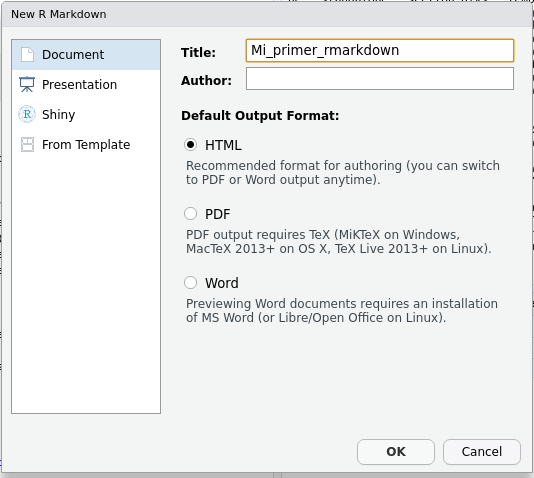
\includegraphics{img/nuevo-rmd.png}

Cuál es el formato de salida de un archivo de R Markdown se determina principalmente con la opción \texttt{output} en el encabezado yaml. Si mirás el encabezado del \href{files/mi-primer-rmarkdown.Rmd}{archivo R Markdown de ejemplo} vas a ver que la opción \texttt{output} dice \texttt{html\_document}.

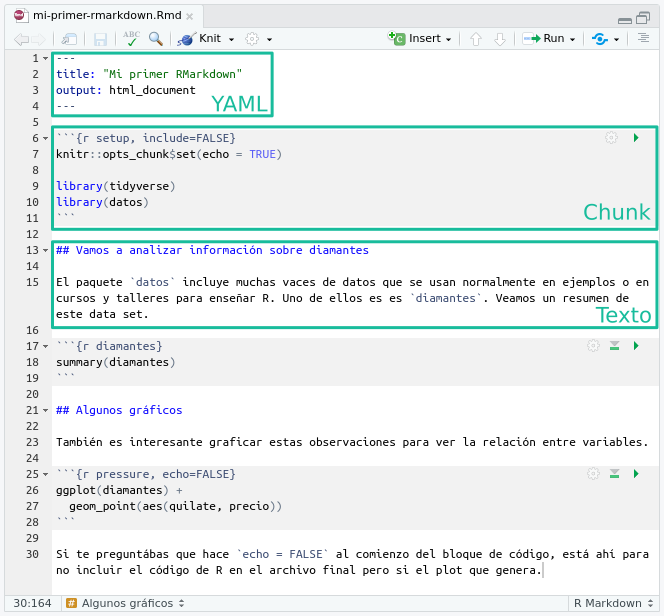
\includegraphics{img/rmd-ejemplo-secciones.png}

Ese \texttt{html\_document} no es otra cosa que una función de \{Rmarkdown\} llamada \texttt{html\_document}. Como te podrás imaginar, \{Rmarkdown\} tiene una serie de otras funciones que definen formatos de salida. Los dos que seguramente te van a servir más son \texttt{pdf\_document} y \texttt{word\_document} que justamente generan PDFs y archivos de Word, respectivamente.

Para crear un documento de R Markdown que genere un archivo PDF basta con cambiar el \texttt{output} en el encabezado por esto:

\begin{Shaded}
\begin{Highlighting}[]
\PreprocessorTok{{-}{-}{-}}
\FunctionTok{output}\KeywordTok{:}\AttributeTok{ pdf\_document}
\PreprocessorTok{{-}{-}{-}}
\end{Highlighting}
\end{Shaded}

Para que el documento se genere correctamente hace falta instalar LaTeX, que es un sistema de composición de textos. Aunque parezca mentira, la mejor forma de instalar LaTeX para usar R Markdown es instalando el paquete \{\href{https://yihui.org/tinytex/}{tinytex}\} con \texttt{install.packages("tinytex")} y luego correr \texttt{tinytex::install\_tinytex()}. Esto va a instalar una versión pequeña de LaTeX en un lugar donde luego \{Rmarkdown\} lo puede usar. Esta es la forma altamente recomendada para generar PDFs con R Markdown que va a evitarte un montón de dolores de cabeza.

Análogamente, podés generar un archivo de word cambiando el \texttt{output} así:

\begin{Shaded}
\begin{Highlighting}[]
\PreprocessorTok{{-}{-}{-}}
\FunctionTok{output}\KeywordTok{:}\AttributeTok{ word\_document}
\PreprocessorTok{{-}{-}{-}}
\end{Highlighting}
\end{Shaded}

Y ya está. En la gran mayoría de los casos no vas a tener que modificar nada más del código ni el texto.

\textbf{Desafío}

Agarrá el reporte que estuviste armando en los desafíos o alguno que usaste durante el curso y compilalo en PDF y luego en Word.

\hypertarget{personalizando-la-salida}{%
\section{Personalizando la salida}\label{personalizando-la-salida}}

Cada función de formato viene con sus opciones de personalización que podés acceder leyendo su documentación. Para ver la documentación de \texttt{html\_document}, usa este comando:

\begin{Shaded}
\begin{Highlighting}[]
\NormalTok{?rmarkdown}\SpecialCharTok{::}\NormalTok{html\_document}
\end{Highlighting}
\end{Shaded}

Vas a ver que tiene un montón de argumentos que modifican la salida. La forma de setear estos argumentos en un documento de R Markdown es, de nuevo, en el encabezado. Cada argumento de la función de salida (\texttt{html\_document} en este caso) es un elemento debajo de la función de output.

Por ejemplo, para que un documento de html tenga una tabla de contenidos hay que setear el argumento \texttt{toc} (de \textbf{t}able \textbf{o}f \textbf{c}ontents) a \texttt{TRUE}. En el encabezado, esto queda así:

\begin{Shaded}
\begin{Highlighting}[]
\PreprocessorTok{{-}{-}{-}}
\FunctionTok{output}\KeywordTok{:}\AttributeTok{ }
\AttributeTok{  }\FunctionTok{html\_document}\KeywordTok{:}
\AttributeTok{    }\FunctionTok{toc}\KeywordTok{:}\AttributeTok{ }\CharTok{TRUE}
\PreprocessorTok{{-}{-}{-}}
\end{Highlighting}
\end{Shaded}

Conviene mirar eso con un poco de detenimiento porque requiere ``traducir'' código de R --cual los argumentos de una función se fijan entre paréntesis y con \texttt{=}-- en código de yaml --donde los argumentos de la función son una lista cuyos elementos se definen con \texttt{:}.

En R lo que vemos como \texttt{html\_document(toc\ =\ TRUE)} se traduce a yaml como

\begin{Shaded}
\begin{Highlighting}[]
\FunctionTok{html\_document}\KeywordTok{:}
\AttributeTok{  }\FunctionTok{toc}\KeywordTok{:}\AttributeTok{ }\CharTok{TRUE}
\end{Highlighting}
\end{Shaded}

Si vas a la ayuda de \texttt{pdf\_document} vas a ver que también tiene un argumento llamado \texttt{toc}. Algunos argumentos son compartidos, lo cual hace que se aún más fácil generar un mismo reporte en muchos formatos haciendo muy pocos cambios.

Una forma rápida de hacer tus informes más vistosos es cambiarle el tema visual. \texttt{html\_document} permite elegir entre una serie de temas usando el argumento \texttt{theme}. Por ejemplo, poniendo esto en el encabezado, generás un documento HTML con un fondo oscuro

\begin{Shaded}
\begin{Highlighting}[]
\FunctionTok{output}\KeywordTok{:}\AttributeTok{ }
\AttributeTok{  }\FunctionTok{html\_document}\KeywordTok{:}
\AttributeTok{    }\FunctionTok{toc}\KeywordTok{:}\AttributeTok{ }\CharTok{TRUE}
\AttributeTok{    }\FunctionTok{theme}\KeywordTok{:}\AttributeTok{ darkly}
\end{Highlighting}
\end{Shaded}

\textbf{Desafío}

Andá a la ayuda de \texttt{html\_document} y fijate cuáles son los valores válidos para el argumento \texttt{theme}. ¡Probá algunos!

\hypertarget{reportes-parametrizados}{%
\section{Reportes parametrizados}\label{reportes-parametrizados}}

Es muy común tener que hacer un reporte cuyo resultado dependa de ciertos parámetros.

Por ejemplo, podrías tener un reporte que analiza la evolución de la expectativa de vida de Argentina con el siguiente código

\begin{Shaded}
\begin{Highlighting}[]
\FunctionTok{library}\NormalTok{(readr)}
\FunctionTok{library}\NormalTok{(dplyr)}
\FunctionTok{library}\NormalTok{(ggplot2)}

\NormalTok{paises }\OtherTok{\textless{}{-}} \FunctionTok{read\_csv}\NormalTok{(}\StringTok{"datos/paises.csv"}\NormalTok{)}

\NormalTok{paises }\SpecialCharTok{\%\textgreater{}\%} 
  \FunctionTok{filter}\NormalTok{(pais }\SpecialCharTok{==} \StringTok{"Argentina"}\NormalTok{) }\SpecialCharTok{\%\textgreater{}\%} 
  \FunctionTok{ggplot}\NormalTok{(}\FunctionTok{aes}\NormalTok{(anio, esperanza\_de\_vida)) }\SpecialCharTok{+}
  \FunctionTok{geom\_line}\NormalTok{()}
\end{Highlighting}
\end{Shaded}

\begin{center}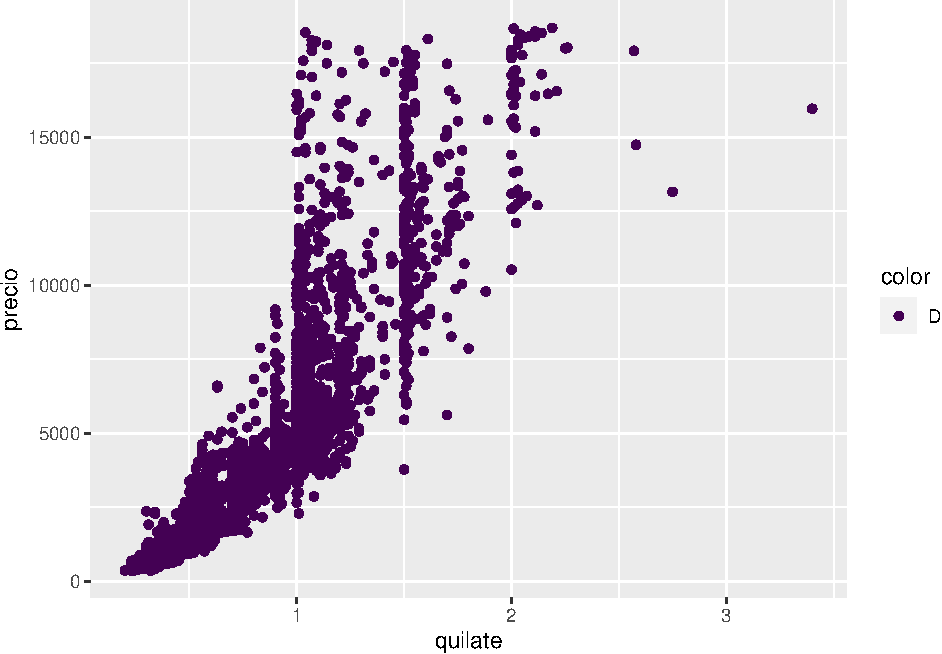
\includegraphics[width=1\linewidth]{DT6_files/figure-latex/unnamed-chunk-72-1} \end{center}

Si ahora querés hacer el mismo reporte pero para Uruguay, tenés que abrir el archivo y modificar la llamada a \texttt{filter} para quedarte sólo con ese país:

\begin{Shaded}
\begin{Highlighting}[]
\FunctionTok{library}\NormalTok{(readr)}
\FunctionTok{library}\NormalTok{(dplyr)}
\FunctionTok{library}\NormalTok{(ggplot2)}

\NormalTok{paises }\OtherTok{\textless{}{-}} \FunctionTok{read\_csv}\NormalTok{(}\StringTok{"datos/paises.csv"}\NormalTok{)}

\NormalTok{paises }\SpecialCharTok{\%\textgreater{}\%} 
  \FunctionTok{filter}\NormalTok{(pais }\SpecialCharTok{==} \StringTok{"Uruguay"}\NormalTok{) }\SpecialCharTok{\%\textgreater{}\%} 
  \FunctionTok{ggplot}\NormalTok{(}\FunctionTok{aes}\NormalTok{(anio, esperanza\_de\_vida)) }\SpecialCharTok{+}
  \FunctionTok{geom\_line}\NormalTok{()}
\end{Highlighting}
\end{Shaded}

Si el reporte es largo y usa el nombre del país en múltiples lugares cambiar ``Argentina'' por ``Uruguay'' puede ser tedioso y propenso a error, ya que te obliga a modificar muchas partes del código. Y si después tenés que hacer el mismo reporte para Chile\ldots{}

En estas situaciones podés crear un reporte parametrizado. La idea es que el reporte tiene una serie de parámetros que puede modificar la salida. Es como si el archivo de R Markdown fuera una gran función con sus argumentos!

Para generar un reporte parametrizado hay que agregar un elemento llamado \texttt{params} al encabezado con la lista de parámetros y sus valores por default.

\begin{Shaded}
\begin{Highlighting}[]
\FunctionTok{params}\KeywordTok{:}
\AttributeTok{  }\FunctionTok{pais}\KeywordTok{:}\AttributeTok{ Argentina}
\end{Highlighting}
\end{Shaded}

Luego, en el código de R vas a tener acceso a una variable llamada \texttt{params} que es una lista que contiene los parámetros y su valor. Para acceder al valor de cada parámetros se usa el operador \texttt{\$} de la siguiente manera:

\begin{Shaded}
\begin{Highlighting}[]
\NormalTok{params}\SpecialCharTok{$}\NormalTok{pais}
\end{Highlighting}
\end{Shaded}

\begin{verbatim}
## [1] "Argentina"
\end{verbatim}

De esta manera, el código original se puede modificar para usar el valor del país almacenado en \texttt{params\$pais}

\begin{Shaded}
\begin{Highlighting}[]
\FunctionTok{library}\NormalTok{(readr)}
\FunctionTok{library}\NormalTok{(dplyr)}
\FunctionTok{library}\NormalTok{(ggplot2)}

\NormalTok{paises }\OtherTok{\textless{}{-}} \FunctionTok{read\_csv}\NormalTok{(}\StringTok{"datos/paises.csv"}\NormalTok{)}

\NormalTok{paises }\SpecialCharTok{\%\textgreater{}\%} 
  \FunctionTok{filter}\NormalTok{(pais }\SpecialCharTok{==}\NormalTok{ params}\SpecialCharTok{$}\NormalTok{pais) }\SpecialCharTok{\%\textgreater{}\%} 
  \FunctionTok{ggplot}\NormalTok{(}\FunctionTok{aes}\NormalTok{(anio, esperanza\_de\_vida)) }\SpecialCharTok{+}
  \FunctionTok{geom\_line}\NormalTok{()}
\end{Highlighting}
\end{Shaded}

Y ahora el mismo código puede funcionar para distintos países. Para crear reportes distintos para cada país sólo hay que modificar el valor del parámetro en el encabezado:

\begin{Shaded}
\begin{Highlighting}[]
\FunctionTok{params}\KeywordTok{:}
\AttributeTok{  }\FunctionTok{pais}\KeywordTok{:}\AttributeTok{ Uruguay}
\end{Highlighting}
\end{Shaded}

\textbf{Desafío}

Agregá al menos un parámetro al reporte que venís armando.

\hypertarget{control-de-chunks}{%
\section{Control de chunks}\label{control-de-chunks}}

Si te acordás, en la sección de \href{10-reportes-I.html}{reportes I} te dijimos que un chunk tiene una pinta como esta:

\begin{verbatim}
```{r nombre-del-chunk}

```
\end{verbatim}

Ponerle nombre al chunk no es obligatorio pero está bueno para tener una idea de qué hace cada uno, lo cual se vuelve más importante a medida que un reporte se vuelve más largo y complejo. Pero lo que no dijimos es que además del nombre, entre las llave se pueden poner un montón de opciones que cambian el comportamiento y la apariencia del resultado del chunk.

Para cambiar las opciones de un chunk, lo único que hay que hacer es listarlas dentro de los corchetes. Por ejemplo:

\begin{verbatim}
```{r nombre-del-chunk, echo = FALSE, message = FALSE}

```
\end{verbatim}

Hay una serie de opciones particularmente importante es la que controla si el código se ejecuta y si el resultado del código va a quedar en el reporte o no:

\begin{itemize}
\item
  \texttt{eval\ =\ FALSE} evita que se corra el código del chunk, de manera que tampoco va a mostrar resultados. Es útil para mostrar códigos de ejemplo si estás escribiendo, por ejemplo un documento para enseñar R.
\item
  \texttt{echo\ =\ FALSE} corre el código del chunk y muestra los resultados, pero oculta el código en el reporte. Esto es útil para escribir reportes para personas que no necesitan ver el código de R que generó el gráfico o tabla.
\item
  \texttt{include\ =\ FALSE} corre el código pero oculta tanto el código como los resultados. Es útil para usar en chunks de configuración general donde cargas las librerías.
\end{itemize}

Si estás escribiendo un informe en el que no querés que se muestre ningún código, agregarle \texttt{echo\ =\ FALSE} a cada chunk nuevo se vuelve tedioso. La solución es cambiar la opción de forma global de manera que aplique a todos los chunks. Esto se hace mediante la función \texttt{knitr::opts\_chunk\$set()}, que setea las opciones globales de los chunks que le siguen. Si queŕes que todos los chunks tengan \texttt{echo\ =\ TRUE} crearías un chunk así:

\begin{verbatim}
```{r setup, include = FALSE}
knitr::opts_chunk$set(echo = TRUE)
```
\end{verbatim}

Generalmente tiene sentido poner esto en el primer chunk de un documento, que como suele ser cuestiones de configuración del reporte, también conviene ponerle \texttt{include\ =\ FALSE}.

Habrás visto que a vece algunas funciones escupen mensajes sobre lo que hacen. Por ejemplo, cuando \texttt{read\_csv} lee un archivo describe el tipo de dato de cada columna:

\begin{Shaded}
\begin{Highlighting}[]
\NormalTok{paises }\OtherTok{\textless{}{-}} \FunctionTok{read\_csv}\NormalTok{(}\StringTok{"datos/paises.csv"}\NormalTok{)}
\end{Highlighting}
\end{Shaded}

\begin{verbatim}
## Rows: 1704 Columns: 6
\end{verbatim}

\begin{verbatim}
## -- Column specification --------------------------------------------------------
## Delimiter: ","
## chr (2): pais, continente
## dbl (4): anio, esperanza_de_vida, poblacion, pib_per_capita
\end{verbatim}

\begin{verbatim}
## 
## i Use `spec()` to retrieve the full column specification for this data.
## i Specify the column types or set `show_col_types = FALSE` to quiet this message.
\end{verbatim}

Esto es útil cuando uno está haciendo trabajo interactivo pero en general no quiere que quede en el reporte. Para que no muestre estos mensajes basta con poner la opción \texttt{message\ =\ FALSE}

\begin{verbatim}
```{r message = FALSE}
paises <- read_csv("datos/paises.csv")
```
\end{verbatim}

En general no pasa nada si ignorás los mensajes. Son cuestiones diagnósticas extra que sirven para que vos, como humano, te enteres de lo que hizo una función. Distinto son las advertencias, o ``warnings''. Una advertencia te está diciendo que hay algo ``raro'' en el código que puede significar que hay algo mal. No llega al nivel de error, que es algo que literalmente ``no computa''. Por ejemplo, \texttt{sqrt} tira una advertencia cuando recibe números negativos.

\begin{Shaded}
\begin{Highlighting}[]
\NormalTok{i }\OtherTok{\textless{}{-}} \FunctionTok{sqrt}\NormalTok{(}\SpecialCharTok{{-}}\DecValTok{1}\NormalTok{)}
\end{Highlighting}
\end{Shaded}

\begin{verbatim}
## Warning in sqrt(-1): NaNs produced
\end{verbatim}

Si un chunk tira una advertencia que es esperable pero no querés que aparezca en el reporte, podés ocultarlas con la opción \texttt{warning\ =\ FALSE}.

\begin{verbatim}
```{r warning = FALSE}
i <- sqrt(-1)
```
\end{verbatim}

Finalmente, una opción tan poderosa como peligrosa es \texttt{cache\ =\ TRUE}. Lo que hace es que en vez de correr el código de un chunk cada vez que \emph{kniteás} el documento, guarda el resultado del chunk en el disco para reutilizar la próxima vez que crees el reporte. Esto es muy cómo si un chunk se un código que tarda mucho en correr. Por ejemplo el siguiente chunk va a tardar 10 minutos en correr la primera vez que knitees el reporte, pero luego va a ser mucho más rápido:

\begin{verbatim}
```{r cache = FALSE}
datos <- funcion_que_tarda_10_minutos(x)
```
\end{verbatim}

\{knitr\} es bastante inteligente y va a invalidar la cache si cambia el código del chunk. Pero, ¿qué pasa si cambiás algo del código previo que cambia el valor de \texttt{x} o incluso el funcionamiento de \texttt{function\_que\_targa\_10\_minutos}? \{knitr\} no se da cuenta y va a usar la cache, resultando que \texttt{datos} va a tener un valor incorrecto. Hay formas de decirle a \{knitr\} de qué depende cada chunk y así obtener una cache más ``inteligente'' pero es algo que se vuelve complicado muy rápido.

El resumen es usar la cache sólo cuando es imprescindible.

\textbf{Desafío}

Guardá el cógido de esta u otra sección yendo a Código → Descargar Rmd arriba de todo a la derecha. Mirá los chunks y las opciones que están puestas. ¿Por qué usamos cada opción en cada chunk?

Anterior
Siguiente

\hypertarget{tablas}{%
\chapter{Tablas}\label{tablas}}

Por defecto, la forma en que R Markdown muestra tablas es bastante feo porque muestra lo que verías si corrieras el código en la consola.

\begin{Shaded}
\begin{Highlighting}[]
\FunctionTok{library}\NormalTok{(dplyr)}
\NormalTok{paises }\OtherTok{\textless{}{-}}\NormalTok{ readr}\SpecialCharTok{::}\FunctionTok{read\_csv}\NormalTok{(}\StringTok{"datos/paises.csv"}\NormalTok{)}
\NormalTok{paises\_seleccion }\OtherTok{\textless{}{-}}\NormalTok{ paises }\SpecialCharTok{\%\textgreater{}\%} 
  \FunctionTok{filter}\NormalTok{(pais }\SpecialCharTok{\%in\%} \FunctionTok{c}\NormalTok{(}\StringTok{"Argentina"}\NormalTok{, }\StringTok{"Uruguay"}\NormalTok{, }\StringTok{"Chile"}\NormalTok{)) }\SpecialCharTok{\%\textgreater{}\%} 
  \FunctionTok{filter}\NormalTok{(anio }\SpecialCharTok{\%in\%} \FunctionTok{c}\NormalTok{(}\DecValTok{2007}\NormalTok{, }\DecValTok{2002}\NormalTok{)) }\SpecialCharTok{\%\textgreater{}\%}
  \FunctionTok{select}\NormalTok{(}\SpecialCharTok{{-}}\NormalTok{continente)}
\NormalTok{paises\_seleccion}
\end{Highlighting}
\end{Shaded}

\begin{verbatim}
## # A tibble: 6 x 5
##   pais       anio esperanza_de_vida poblacion pib_per_capita
##   <chr>     <dbl>             <dbl>     <dbl>          <dbl>
## 1 Argentina  2002              74.3  38331121          8798.
## 2 Argentina  2007              75.3  40301927         12779.
## 3 Chile      2002              77.9  15497046         10779.
## 4 Chile      2007              78.6  16284741         13172.
## 5 Uruguay    2002              75.3   3363085          7727.
## 6 Uruguay    2007              76.4   3447496         10611.
\end{verbatim}

\hypertarget{tablas-simples-con-kable}{%
\section{\texorpdfstring{Tablas simples con \texttt{kable}}{Tablas simples con kable}}\label{tablas-simples-con-kable}}

Existen varios paquetes para mostrar tablas lindas pero una forma simple y sin vueltas es usando la función \texttt{kable} del paquete \{knitr\}.
Sólo usando esta función ya devuelve una tabla más que razonable:

\begin{Shaded}
\begin{Highlighting}[]
\FunctionTok{library}\NormalTok{(knitr)}
\FunctionTok{kable}\NormalTok{(paises\_seleccion)}
\end{Highlighting}
\end{Shaded}

\begin{tabular}{l|r|r|r|r}
\hline
pais & anio & esperanza\_de\_vida & poblacion & pib\_per\_capita\\
\hline
Argentina & 2002 & 74.340 & 38331121 & 8797.641\\
\hline
Argentina & 2007 & 75.320 & 40301927 & 12779.380\\
\hline
Chile & 2002 & 77.860 & 15497046 & 10778.784\\
\hline
Chile & 2007 & 78.553 & 16284741 & 13171.639\\
\hline
Uruguay & 2002 & 75.307 & 3363085 & 7727.002\\
\hline
Uruguay & 2007 & 76.384 & 3447496 & 10611.463\\
\hline
\end{tabular}

La mayoría de las veces, el nombre de las columnas que queremos mostrar no va a ser igual que el nombre de las columnas en R.
En la tabla \texttt{paises}, los nombres están en minúscula, sin espacios y sin ``caracteres especiales'' como ``ñ'' o ``í''.
Esto es útil para comunicarse con R, pero no está bueno para comunicados a seres humanos.
El argumento \texttt{col.names} permite especificar el nombre de las columnas para mostrar:

\begin{Shaded}
\begin{Highlighting}[]
\FunctionTok{kable}\NormalTok{(paises\_seleccion, }
      \AttributeTok{col.names =} \FunctionTok{c}\NormalTok{(}\StringTok{"País"}\NormalTok{, }\StringTok{"Año"}\NormalTok{, }\StringTok{"Esperanza de vida"}\NormalTok{, }\StringTok{"Población"}\NormalTok{, }\StringTok{"PBI per cápita"}\NormalTok{))}
\end{Highlighting}
\end{Shaded}

\begin{tabular}{l|r|r|r|r}
\hline
País & Año & Esperanza de vida & Población & PBI per cápita\\
\hline
Argentina & 2002 & 74.340 & 38331121 & 8797.641\\
\hline
Argentina & 2007 & 75.320 & 40301927 & 12779.380\\
\hline
Chile & 2002 & 77.860 & 15497046 & 10778.784\\
\hline
Chile & 2007 & 78.553 & 16284741 & 13171.639\\
\hline
Uruguay & 2002 & 75.307 & 3363085 & 7727.002\\
\hline
Uruguay & 2007 & 76.384 & 3447496 & 10611.463\\
\hline
\end{tabular}

En Español, en general usamos la coma para separar los decimales y el punto como separador de miles.
Para eso, hay que modificar el argumento \texttt{format.args} de esta manera:

\begin{Shaded}
\begin{Highlighting}[]
\FunctionTok{kable}\NormalTok{(paises\_seleccion, }
      \AttributeTok{col.names =} \FunctionTok{c}\NormalTok{(}\StringTok{"País"}\NormalTok{, }\StringTok{"Año"}\NormalTok{, }\StringTok{"Esperanza de vida"}\NormalTok{, }\StringTok{"Población"}\NormalTok{, }\StringTok{"PBI per cápita"}\NormalTok{),}
      \AttributeTok{format.args =} \FunctionTok{list}\NormalTok{(}\AttributeTok{decimal.mark =} \StringTok{","}\NormalTok{, }\AttributeTok{big.mark =} \StringTok{"."}\NormalTok{))}
\end{Highlighting}
\end{Shaded}

\begin{tabular}{l|r|r|r|r}
\hline
País & Año & Esperanza de vida & Población & PBI per cápita\\
\hline
Argentina & 2.002 & 74,340 & 38.331.121 & 8.797,641\\
\hline
Argentina & 2.007 & 75,320 & 40.301.927 & 12.779,380\\
\hline
Chile & 2.002 & 77,860 & 15.497.046 & 10.778,784\\
\hline
Chile & 2.007 & 78,553 & 16.284.741 & 13.171,639\\
\hline
Uruguay & 2.002 & 75,307 & 3.363.085 & 7.727,002\\
\hline
Uruguay & 2.007 & 76,384 & 3.447.496 & 10.611,463\\
\hline
\end{tabular}

Uff\ldots{} pero ponerle el punto de miles a los años queda raro.
La solución es convertir la columna \texttt{anio} en caracter.
De esta manera, no se ve afectada por el formato numérico.

\begin{Shaded}
\begin{Highlighting}[]
\NormalTok{paises\_seleccion }\SpecialCharTok{\%\textgreater{}\%} 
  \FunctionTok{mutate}\NormalTok{(}\AttributeTok{anio =} \FunctionTok{as.character}\NormalTok{(anio)) }\SpecialCharTok{\%\textgreater{}\%} 
  \FunctionTok{kable}\NormalTok{(}\AttributeTok{col.names =} \FunctionTok{c}\NormalTok{(}\StringTok{"País"}\NormalTok{, }\StringTok{"Año"}\NormalTok{, }\StringTok{"Esperanza de vida"}\NormalTok{, }\StringTok{"Población"}\NormalTok{, }\StringTok{"PBI per cápita"}\NormalTok{),}
        \AttributeTok{format.args =} \FunctionTok{list}\NormalTok{(}\AttributeTok{decimal.mark =} \StringTok{","}\NormalTok{, }\AttributeTok{big.mark =} \StringTok{"."}\NormalTok{))}
\end{Highlighting}
\end{Shaded}

\begin{tabular}{l|l|r|r|r}
\hline
País & Año & Esperanza de vida & Población & PBI per cápita\\
\hline
Argentina & 2002 & 74,340 & 38.331.121 & 8.797,641\\
\hline
Argentina & 2007 & 75,320 & 40.301.927 & 12.779,380\\
\hline
Chile & 2002 & 77,860 & 15.497.046 & 10.778,784\\
\hline
Chile & 2007 & 78,553 & 16.284.741 & 13.171,639\\
\hline
Uruguay & 2002 & 75,307 & 3.363.085 & 7.727,002\\
\hline
Uruguay & 2007 & 76,384 & 3.447.496 & 10.611,463\\
\hline
\end{tabular}

hacer \texttt{kable}, que es una función diseñada para ser simple y hacer pocas cosas.
Para hacer cosas un poco mas complicadas está el paquete \{kableExtra\}.

\hypertarget{supertablas-con-kableextra}{%
\section{Supertablas con \{kableExtra\}}\label{supertablas-con-kableextra}}

El paquete \{kableExtra\}, como su nombre lo indica, nació para extender el poder de la función \texttt{kable}.

\begin{Shaded}
\begin{Highlighting}[]
\FunctionTok{library}\NormalTok{(kableExtra)  }\CommentTok{\# instalar con install.packages("kableExtra")}
\end{Highlighting}
\end{Shaded}

\begin{verbatim}
## 
## Attaching package: 'kableExtra'
\end{verbatim}

\begin{verbatim}
## The following object is masked from 'package:dplyr':
## 
##     group_rows
\end{verbatim}

\begin{Shaded}
\begin{Highlighting}[]
\NormalTok{paises\_tabla }\OtherTok{\textless{}{-}}\NormalTok{ paises\_seleccion }\SpecialCharTok{\%\textgreater{}\%} 
  \FunctionTok{mutate}\NormalTok{(}\AttributeTok{anio =} \FunctionTok{as.character}\NormalTok{(anio)) }\SpecialCharTok{\%\textgreater{}\%} 
  \FunctionTok{kable}\NormalTok{(}\AttributeTok{col.names =} \FunctionTok{c}\NormalTok{(}\StringTok{"País"}\NormalTok{, }\StringTok{"Año"}\NormalTok{, }\StringTok{"Esperanza de vida"}\NormalTok{, }\StringTok{"Población"}\NormalTok{, }\StringTok{"PBI per cápita"}\NormalTok{),}
        \AttributeTok{format.args =} \FunctionTok{list}\NormalTok{(}\AttributeTok{decimal.mark =} \StringTok{","}\NormalTok{, }\AttributeTok{big.mark =} \StringTok{"."}\NormalTok{))}
\end{Highlighting}
\end{Shaded}

La primera columna de la tabla de arriba es un tanto redundante.
Sería mejor agrupar las filas según el país.
Esto se consigue con la función \texttt{collapse\_rows}:

\begin{Shaded}
\begin{Highlighting}[]
\NormalTok{paises\_tabla }\SpecialCharTok{\%\textgreater{}\%} 
  \FunctionTok{collapse\_rows}\NormalTok{(}\AttributeTok{columns =} \DecValTok{1}\NormalTok{, }\AttributeTok{valign =} \StringTok{"top"}\NormalTok{)  }\SpecialCharTok{\%\textgreater{}\%} 
  \FunctionTok{kable\_styling}\NormalTok{() }
\end{Highlighting}
\end{Shaded}

\begin{table}
\centering
\begin{tabular}{l|l|r|r|r}
\hline
País & Año & Esperanza de vida & Población & PBI per cápita\\
\hline
 & 2002 & 74,340 & 38.331.121 & 8.797,641\\
\cline{2-5}
\multirow[t]{-2}{*}{\raggedright\arraybackslash Argentina} & 2007 & 75,320 & 40.301.927 & 12.779,380\\
\cline{1-5}
 & 2002 & 77,860 & 15.497.046 & 10.778,784\\
\cline{2-5}
\multirow[t]{-2}{*}{\raggedright\arraybackslash Chile} & 2007 & 78,553 & 16.284.741 & 13.171,639\\
\cline{1-5}
 & 2002 & 75,307 & 3.363.085 & 7.727,002\\
\cline{2-5}
\multirow[t]{-2}{*}{\raggedright\arraybackslash Uruguay} & 2007 & 76,384 & 3.447.496 & 10.611,463\\
\hline
\end{tabular}
\end{table}

El primer argumento es el número de la columna que queremos agrupar.
En este caso, la columna \texttt{pais} es la primera.
El segundo argumento es la alineación vertical.
Por defecto, \texttt{collapse\_rows} pone las etiquetas en el centro, pero la convención más general es ponerlas arriba.

¿Qué es esa \texttt{kable\_styling()}?
\{kableExtra\} permite cambiar el estilo de las tablas muy fácilmente.
\texttt{kable\_styling} es el estilo por defecto, que es igual al que produce \texttt{kable}, pero tiene muchos otros.
Si viste tablas hechas en LaTeX, quizás este estilo te resulte familiar:

\begin{Shaded}
\begin{Highlighting}[]
\NormalTok{paises\_tabla }\SpecialCharTok{\%\textgreater{}\%} 
  \FunctionTok{collapse\_rows}\NormalTok{(}\AttributeTok{columns =} \DecValTok{1}\NormalTok{, }\AttributeTok{valign =} \StringTok{"top"}\NormalTok{)  }\SpecialCharTok{\%\textgreater{}\%} 
  \FunctionTok{kable\_classic\_2}\NormalTok{()}
\end{Highlighting}
\end{Shaded}

\begin{table}
\centering
\begin{tabular}{l|l|r|r|r}
\hline
País & Año & Esperanza de vida & Población & PBI per cápita\\
\hline
 & 2002 & 74,340 & 38.331.121 & 8.797,641\\
\cline{2-5}
\multirow[t]{-2}{*}{\raggedright\arraybackslash Argentina} & 2007 & 75,320 & 40.301.927 & 12.779,380\\
\cline{1-5}
 & 2002 & 77,860 & 15.497.046 & 10.778,784\\
\cline{2-5}
\multirow[t]{-2}{*}{\raggedright\arraybackslash Chile} & 2007 & 78,553 & 16.284.741 & 13.171,639\\
\cline{1-5}
 & 2002 & 75,307 & 3.363.085 & 7.727,002\\
\cline{2-5}
\multirow[t]{-2}{*}{\raggedright\arraybackslash Uruguay} & 2007 & 76,384 & 3.447.496 & 10.611,463\\
\hline
\end{tabular}
\end{table}

La función \texttt{column\_spec} permite cambiar los parámetros gráficos de una o más columnas.
En este caso cambiamos la primera columna (\texttt{column\ =\ 1}) para que las palabras aparezcan italizadas (\texttt{italic\ =\ TRUE}):

\begin{Shaded}
\begin{Highlighting}[]
\NormalTok{paises\_tabla }\SpecialCharTok{\%\textgreater{}\%} 
  \FunctionTok{column\_spec}\NormalTok{(}\AttributeTok{column =} \DecValTok{1}\NormalTok{, }\AttributeTok{italic =} \ConstantTok{TRUE}\NormalTok{) }\SpecialCharTok{\%\textgreater{}\%}
  \FunctionTok{collapse\_rows}\NormalTok{(}\AttributeTok{columns =} \DecValTok{1}\NormalTok{, }\AttributeTok{valign =} \StringTok{"top"}\NormalTok{)  }\SpecialCharTok{\%\textgreater{}\%}
  \FunctionTok{kable\_styling}\NormalTok{() }
\end{Highlighting}
\end{Shaded}

\begin{table}
\centering
\begin{tabular}{>{}l|l|r|r|r}
\hline
País & Año & Esperanza de vida & Población & PBI per cápita\\
\hline
 & 2002 & 74,340 & 38.331.121 & 8.797,641\\
\cline{2-5}
\multirow[t]{-2}{*}{\raggedright\arraybackslash \em{Argentina}} & 2007 & 75,320 & 40.301.927 & 12.779,380\\
\cline{1-5}
 & 2002 & 77,860 & 15.497.046 & 10.778,784\\
\cline{2-5}
\multirow[t]{-2}{*}{\raggedright\arraybackslash \em{Chile}} & 2007 & 78,553 & 16.284.741 & 13.171,639\\
\cline{1-5}
 & 2002 & 75,307 & 3.363.085 & 7.727,002\\
\cline{2-5}
\multirow[t]{-2}{*}{\raggedright\arraybackslash \em{Uruguay}} & 2007 & 76,384 & 3.447.496 & 10.611,463\\
\hline
\end{tabular}
\end{table}

Lo notable de \texttt{column\_spec} es que en sus argumentos se pueden poner vectores de manera de generar formato condicional.
Para resaltar con negrita únicamente el país ``Argentina'':

\begin{Shaded}
\begin{Highlighting}[]
\NormalTok{paises\_tabla }\SpecialCharTok{\%\textgreater{}\%} 
  \FunctionTok{column\_spec}\NormalTok{(}\AttributeTok{column =} \DecValTok{1}\NormalTok{, }\AttributeTok{bold =}\NormalTok{ (paises\_seleccion}\SpecialCharTok{$}\NormalTok{pais }\SpecialCharTok{==} \StringTok{"Argentina"}\NormalTok{)) }\SpecialCharTok{\%\textgreater{}\%}
  \FunctionTok{collapse\_rows}\NormalTok{(}\AttributeTok{columns =} \DecValTok{1}\NormalTok{, }\AttributeTok{valign =} \StringTok{"top"}\NormalTok{)  }\SpecialCharTok{\%\textgreater{}\%}
  \FunctionTok{kable\_styling}\NormalTok{() }
\end{Highlighting}
\end{Shaded}

\begin{table}
\centering
\begin{tabular}{>{}l|l|r|r|r}
\hline
País & Año & Esperanza de vida & Población & PBI per cápita\\
\hline
 & 2002 & 74,340 & 38.331.121 & 8.797,641\\
\cline{2-5}
\multirow[t]{-2}{*}{\raggedright\arraybackslash \textbf{Argentina}} & 2007 & 75,320 & 40.301.927 & 12.779,380\\
\cline{1-5}
 & 2002 & 77,860 & 15.497.046 & 10.778,784\\
\cline{2-5}
\multirow[t]{-2}{*}{\raggedright\arraybackslash Chile} & 2007 & 78,553 & 16.284.741 & 13.171,639\\
\cline{1-5}
 & 2002 & 75,307 & 3.363.085 & 7.727,002\\
\cline{2-5}
\multirow[t]{-2}{*}{\raggedright\arraybackslash Uruguay} & 2007 & 76,384 & 3.447.496 & 10.611,463\\
\hline
\end{tabular}
\end{table}

Conviene detenerse para mirar un poco con detalle el código.
La llamada a \texttt{column\_spec} está cambiando el formato de la columna 1.
En particular, va a determinar si el texto es en negrita (bold) o no.
Y la forma para determinarlo es el vector \texttt{paises\$pais\ ==\ "Argentina"}.
¿Qué es ese vector?

\begin{Shaded}
\begin{Highlighting}[]
\NormalTok{paises\_seleccion}\SpecialCharTok{$}\NormalTok{pais }\SpecialCharTok{==} \StringTok{"Argentina"}
\end{Highlighting}
\end{Shaded}

\begin{verbatim}
## [1]  TRUE  TRUE FALSE FALSE FALSE FALSE
\end{verbatim}

Por lo tanto, \texttt{column\_spec(column\ =\ 1,\ bold\ =\ (paises\$pais\ ==\ "Argentina"))} va a hacer que las dos primera filas de la columna uno estén en negrita, y las demás no.
Luego, \texttt{collapse\_rows} colapsa las filas según el país y entonces esas dos primeras filas se transforman en una.

Esto da un montón de flexibilidad en el estilo del texto.
Por ejemplo, se puede hacer que el color del texto cambie según el valor usando \texttt{column\_spec} y \texttt{spec\_color}.

\begin{Shaded}
\begin{Highlighting}[]
\NormalTok{paises\_tabla }\SpecialCharTok{\%\textgreater{}\%} 
  \FunctionTok{column\_spec}\NormalTok{(}\DecValTok{3}\NormalTok{, }\AttributeTok{color =} \FunctionTok{spec\_color}\NormalTok{(paises\_seleccion}\SpecialCharTok{$}\NormalTok{esperanza\_de\_vida)) }\SpecialCharTok{\%\textgreater{}\%} 
  \FunctionTok{collapse\_rows}\NormalTok{(}\AttributeTok{columns =} \DecValTok{1}\NormalTok{, }\AttributeTok{valign =} \StringTok{"top"}\NormalTok{)  }\SpecialCharTok{\%\textgreater{}\%}
  \FunctionTok{kable\_styling}\NormalTok{() }
\end{Highlighting}
\end{Shaded}

\begin{table}
\centering
\begin{tabular}{l|l|>{}r|r|r}
\hline
País & Año & Esperanza de vida & Población & PBI per cápita\\
\hline
 & 2002 & \textcolor[HTML]{440154}{74,340} & 38.331.121 & 8.797,641\\
\cline{2-5}
\multirow[t]{-2}{*}{\raggedright\arraybackslash Argentina} & 2007 & \textcolor[HTML]{3D4D8A}{75,320} & 40.301.927 & 12.779,380\\
\cline{1-5}
 & 2002 & \textcolor[HTML]{90D743}{77,860} & 15.497.046 & 10.778,784\\
\cline{2-5}
\multirow[t]{-2}{*}{\raggedright\arraybackslash Chile} & 2007 & \textcolor[HTML]{FDE725}{78,553} & 16.284.741 & 13.171,639\\
\cline{1-5}
 & 2002 & \textcolor[HTML]{3D4D8A}{75,307} & 3.363.085 & 7.727,002\\
\cline{2-5}
\multirow[t]{-2}{*}{\raggedright\arraybackslash Uruguay} & 2007 & \textcolor[HTML]{228D8D}{76,384} & 3.447.496 & 10.611,463\\
\hline
\end{tabular}
\end{table}

La función nueva, \texttt{spec\_color} genera colores a partir de un vector.
Podés ver cómo funciona en esta linea:

\begin{Shaded}
\begin{Highlighting}[]
\FunctionTok{spec\_color}\NormalTok{(paises\_seleccion}\SpecialCharTok{$}\NormalTok{esperanza\_de\_vida)}
\end{Highlighting}
\end{Shaded}

\begin{verbatim}
## [1] "#440154FF" "#3D4D8AFF" "#90D743FF" "#FDE725FF" "#3D4D8AFF" "#228D8DFF"
\end{verbatim}

Esos números son representaciones en hexadecimal de los colores que ves en la tabla.
Podés pasarle cualquier serie de colores, no sólo la creada con \texttt{spec\_color}.

Así como se puede cambiar el estilo de las columnas con \texttt{column\_spec}, se puede cambiar el estilo de las filas con \texttt{row\_spec}.
Por ejemplo, se puede resaltar cada 2 líneas con este código:

\begin{Shaded}
\begin{Highlighting}[]
\NormalTok{paises\_tabla }\SpecialCharTok{\%\textgreater{}\%} 
  \FunctionTok{row\_spec}\NormalTok{(}\AttributeTok{row =} \FunctionTok{seq}\NormalTok{(}\DecValTok{2}\NormalTok{, }\FunctionTok{nrow}\NormalTok{(paises\_seleccion), }\AttributeTok{by =} \DecValTok{2}\NormalTok{), }\AttributeTok{background =} \StringTok{"azure"}\NormalTok{) }\SpecialCharTok{\%\textgreater{}\%} 
  \FunctionTok{collapse\_rows}\NormalTok{(}\AttributeTok{columns =} \DecValTok{1}\NormalTok{, }\AttributeTok{valign =} \StringTok{"top"}\NormalTok{)  }\SpecialCharTok{\%\textgreater{}\%}
  \FunctionTok{kable\_styling}\NormalTok{() }
\end{Highlighting}
\end{Shaded}

\begin{table}
\centering
\begin{tabular}{l|l|r|r|r}
\hline
País & Año & Esperanza de vida & Población & PBI per cápita\\
\hline
Argentina & 2002 & 74,340 & 38.331.121 & 8.797,641\\
\cline{1-5}
\cellcolor{azure}{Argentina} & \cellcolor{azure}{2007} & \cellcolor{azure}{75,320} & \cellcolor{azure}{40.301.927} & \cellcolor{azure}{12.779,380}\\
\cline{1-5}
Chile & 2002 & 77,860 & 15.497.046 & 10.778,784\\
\cline{1-5}
\cellcolor{azure}{Chile} & \cellcolor{azure}{2007} & \cellcolor{azure}{78,553} & \cellcolor{azure}{16.284.741} & \cellcolor{azure}{13.171,639}\\
\cline{1-5}
Uruguay & 2002 & 75,307 & 3.363.085 & 7.727,002\\
\cline{1-5}
\cellcolor{azure}{Uruguay} & \cellcolor{azure}{2007} & \cellcolor{azure}{76,384} & \cellcolor{azure}{3.447.496} & \cellcolor{azure}{10.611,463}\\
\hline
\end{tabular}
\end{table}

\texttt{row\_spec} está cambiando el fondo (background) al color ``azure'' (que es ese celestito) a las filas indicadas por \texttt{seq(2,\ nrow(paises\_seleccion),\ by\ =\ 2)}.
¿Qué es eso?
\texttt{seq} genera una secuencia (de \textbf{seq}uence) de números empezando en 2, terminando en la cantidad de filas de \texttt{paises\_seleccion} y saltando de a dos.
En resumen:

\begin{Shaded}
\begin{Highlighting}[]
\FunctionTok{seq}\NormalTok{(}\DecValTok{2}\NormalTok{, }\FunctionTok{nrow}\NormalTok{(paises\_seleccion), }\AttributeTok{by =} \DecValTok{2}\NormalTok{)}
\end{Highlighting}
\end{Shaded}

\begin{verbatim}
## [1] 2 4 6
\end{verbatim}

Como caso especial, se puede usar \texttt{row\ =\ 0} en \texttt{row\_spec} para cambiar el formato del encabezado.

\begin{Shaded}
\begin{Highlighting}[]
\NormalTok{paises\_tabla }\SpecialCharTok{\%\textgreater{}\%} 
  \FunctionTok{row\_spec}\NormalTok{(}\AttributeTok{row =} \DecValTok{0}\NormalTok{, }\AttributeTok{underline =} \ConstantTok{TRUE}\NormalTok{) }\SpecialCharTok{\%\textgreater{}\%} 
  \FunctionTok{collapse\_rows}\NormalTok{(}\AttributeTok{columns =} \DecValTok{1}\NormalTok{, }\AttributeTok{valign =} \StringTok{"top"}\NormalTok{)  }\SpecialCharTok{\%\textgreater{}\%}
  \FunctionTok{kable\_styling}\NormalTok{() }
\end{Highlighting}
\end{Shaded}

\begin{table}
\centering
\begin{tabular}{l|l|r|r|r}
\hline
\underline{País} & \underline{Año} & \underline{Esperanza de vida} & \underline{Población} & \underline{PBI per cápita}\\
\hline
 & 2002 & 74,340 & 38.331.121 & 8.797,641\\
\cline{2-5}
\multirow[t]{-2}{*}{\raggedright\arraybackslash Argentina} & 2007 & 75,320 & 40.301.927 & 12.779,380\\
\cline{1-5}
 & 2002 & 77,860 & 15.497.046 & 10.778,784\\
\cline{2-5}
\multirow[t]{-2}{*}{\raggedright\arraybackslash Chile} & 2007 & 78,553 & 16.284.741 & 13.171,639\\
\cline{1-5}
 & 2002 & 75,307 & 3.363.085 & 7.727,002\\
\cline{2-5}
\multirow[t]{-2}{*}{\raggedright\arraybackslash Uruguay} & 2007 & 76,384 & 3.447.496 & 10.611,463\\
\hline
\end{tabular}
\end{table}

Esto es sólo una mínima parte de lo que se puede hacer con el paquete \{kableExtra\}.
Para ejemplos mucho más detallados, te recomendamos leer \href{https://cran.r-project.org/web/packages/kableExtra/vignettes/awesome_table_in_html.html}{la viñeta completa}

\hypertarget{apariencia-de-gruxe1ficos}{%
\chapter{Apariencia de gráficos}\label{apariencia-de-gruxe1ficos}}

\begin{Shaded}
\begin{Highlighting}[]
\FunctionTok{library}\NormalTok{(ggplot2)}
\FunctionTok{library}\NormalTok{(dplyr)}
\end{Highlighting}
\end{Shaded}

\hypertarget{escalas}{%
\section{Escalas}\label{escalas}}

\href{06-graficos-I.html}{Previamente} comentamos que el \emph{mapeo} de una variable en un elemento geométrico, por ejemplo cuando le asignamos distintos colores a los puntos que representan cada continente, usa una \textbf{escala} para definir, en este caso, que color le corresponde a cada elemento.

También cambiamos la apariencia del relleno (o \texttt{fill}) de barras y la forma de los puntos (o \texttt{shape}).
Para esto, \{ggplot2\} siempre usa una escala que podemos modificar de acuerdo a nuestro gusto y teniendo en cuenta cómo queremos comunicar nuestros resultados.

Por supuesto, modificar una escala implica sumar una nueva capa al gráfico sumando una nueva función.
Todas las funciones de escala comienzan con \texttt{scale} (de escala en inglés), el tipo de apariencia que queremos modificar (\texttt{color}, \texttt{fill}, \texttt{shape}, etc) y en muchos casos un nombre o una característica de esa escala.

Para mostrar como funciona, vamos a utilizar la base de datos de países y con suerte al final de este documento tendremos un gráfico listo para publicar.

\begin{Shaded}
\begin{Highlighting}[]
\NormalTok{paises }\OtherTok{\textless{}{-}}\NormalTok{ readr}\SpecialCharTok{::}\FunctionTok{read\_csv}\NormalTok{(}\StringTok{"datos/paises.csv"}\NormalTok{)}
\end{Highlighting}
\end{Shaded}

\begin{verbatim}
## Rows: 1704 Columns: 6
\end{verbatim}

\begin{verbatim}
## -- Column specification --------------------------------------------------------
## Delimiter: ","
## chr (2): pais, continente
## dbl (4): anio, esperanza_de_vida, poblacion, pib_per_capita
\end{verbatim}

\begin{verbatim}
## 
## i Use `spec()` to retrieve the full column specification for this data.
## i Specify the column types or set `show_col_types = FALSE` to quiet this message.
\end{verbatim}

\begin{Shaded}
\begin{Highlighting}[]
\NormalTok{paises }\SpecialCharTok{\%\textgreater{}\%} 
  \FunctionTok{filter}\NormalTok{(anio }\SpecialCharTok{==} \DecValTok{2007}\NormalTok{) }\SpecialCharTok{\%\textgreater{}\%} 
  \FunctionTok{ggplot}\NormalTok{(}\FunctionTok{aes}\NormalTok{(pib\_per\_capita, esperanza\_de\_vida)) }\SpecialCharTok{+}
  \FunctionTok{geom\_point}\NormalTok{()}
\end{Highlighting}
\end{Shaded}

\begin{center}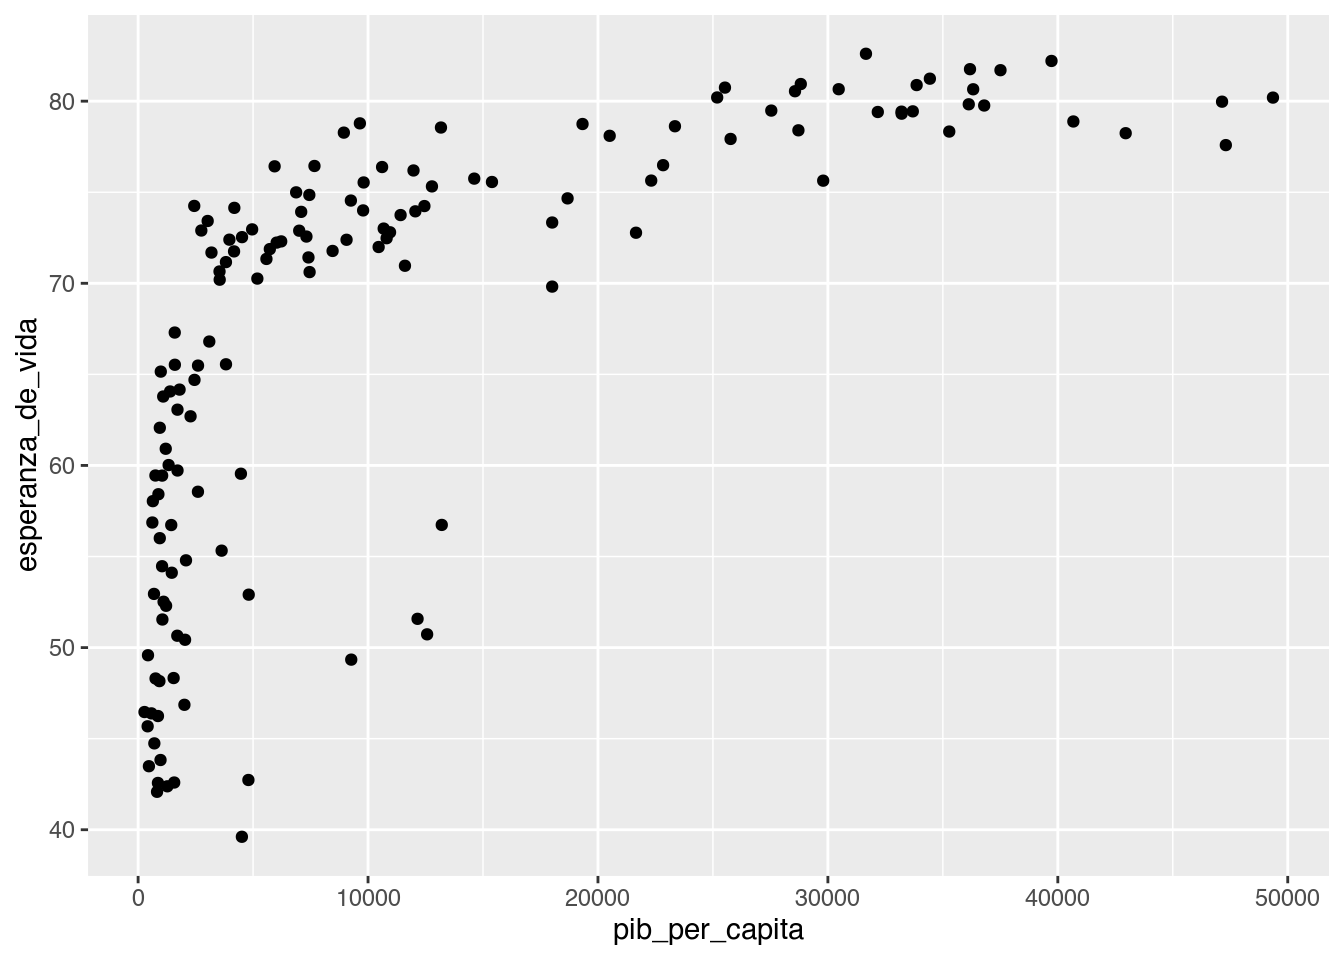
\includegraphics[width=1\linewidth]{DT6_files/figure-latex/unnamed-chunk-97-1} \end{center}

\hypertarget{escala-de-colores-y-otras}{%
\subsection{Escala de colores y otras}\label{escala-de-colores-y-otras}}

Lo primero que podemos hacer es cambiar el color de los puntos de a cuerdo al continente.

\begin{Shaded}
\begin{Highlighting}[]
\NormalTok{paises }\SpecialCharTok{\%\textgreater{}\%} 
  \FunctionTok{filter}\NormalTok{(anio }\SpecialCharTok{==} \DecValTok{2007}\NormalTok{) }\SpecialCharTok{\%\textgreater{}\%} 
  \FunctionTok{ggplot}\NormalTok{(}\FunctionTok{aes}\NormalTok{(pib\_per\_capita, esperanza\_de\_vida)) }\SpecialCharTok{+}
  \FunctionTok{geom\_point}\NormalTok{(}\FunctionTok{aes}\NormalTok{(}\AttributeTok{color =}\NormalTok{ continente))}
\end{Highlighting}
\end{Shaded}

\begin{center}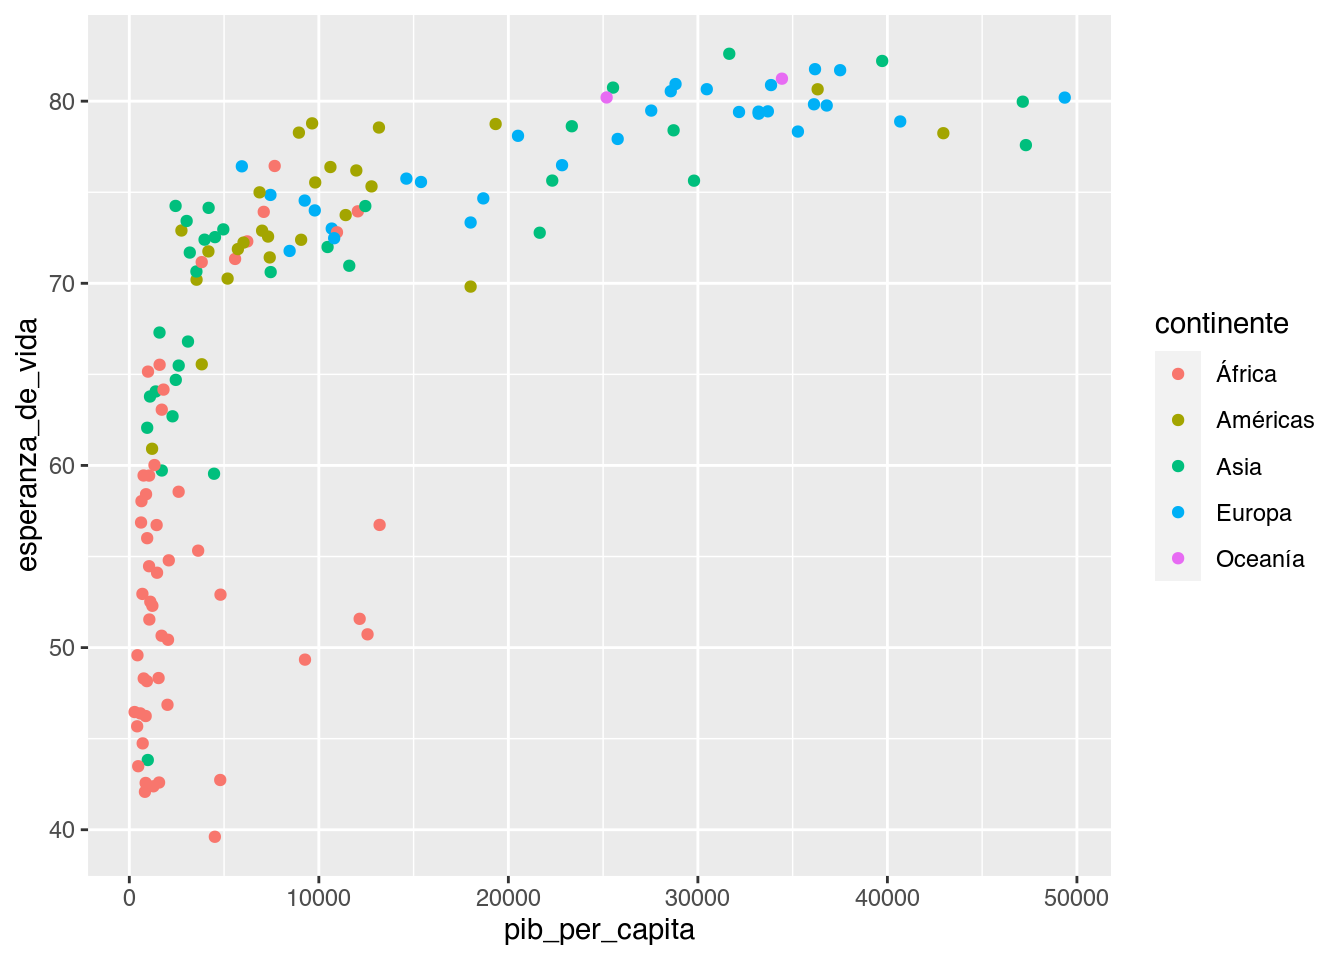
\includegraphics[width=1\linewidth]{DT6_files/figure-latex/unnamed-chunk-98-1} \end{center}

Pero esta escala de colores que usa \{ggplot2\} por defecto no es de las mejores, de hecho las personas que tienen daltonísmo muy posiblemente no logren diferenciar todos los puntos.
Una escala o paleta de colores muy usada es \href{https://cran.r-project.org/web/packages/viridis/vignettes/intro-to-viridis.html}{\textbf{viridis}} que fue creada justamente para resolver este y otros problemas.
También existe otra gran familia de paletas de colores llamada \href{https://colorbrewer2.org/}{\textbf{ColorBrewer}}.

Vamos a probar la paleta ``Dark2'' de ColorBrewer, esta paleta es \emph{qualitativa} y es justo lo que necesitamos para identificar elementos en categorías como los continentes.
Cómo estamos modificando el \emph{color}, la función a usar será \texttt{scale\_color\_brewer()}:

\begin{Shaded}
\begin{Highlighting}[]
\NormalTok{paises }\SpecialCharTok{\%\textgreater{}\%} 
  \FunctionTok{filter}\NormalTok{(anio }\SpecialCharTok{==} \DecValTok{2007}\NormalTok{) }\SpecialCharTok{\%\textgreater{}\%} 
  \FunctionTok{ggplot}\NormalTok{(}\FunctionTok{aes}\NormalTok{(pib\_per\_capita, esperanza\_de\_vida)) }\SpecialCharTok{+}
  \FunctionTok{geom\_point}\NormalTok{(}\FunctionTok{aes}\NormalTok{(}\AttributeTok{color =}\NormalTok{ continente)) }\SpecialCharTok{+}
  \FunctionTok{scale\_color\_brewer}\NormalTok{(}\AttributeTok{type =} \StringTok{"qual"}\NormalTok{, }\AttributeTok{palette =} \StringTok{"Dark2"}\NormalTok{)}
\end{Highlighting}
\end{Shaded}

\begin{center}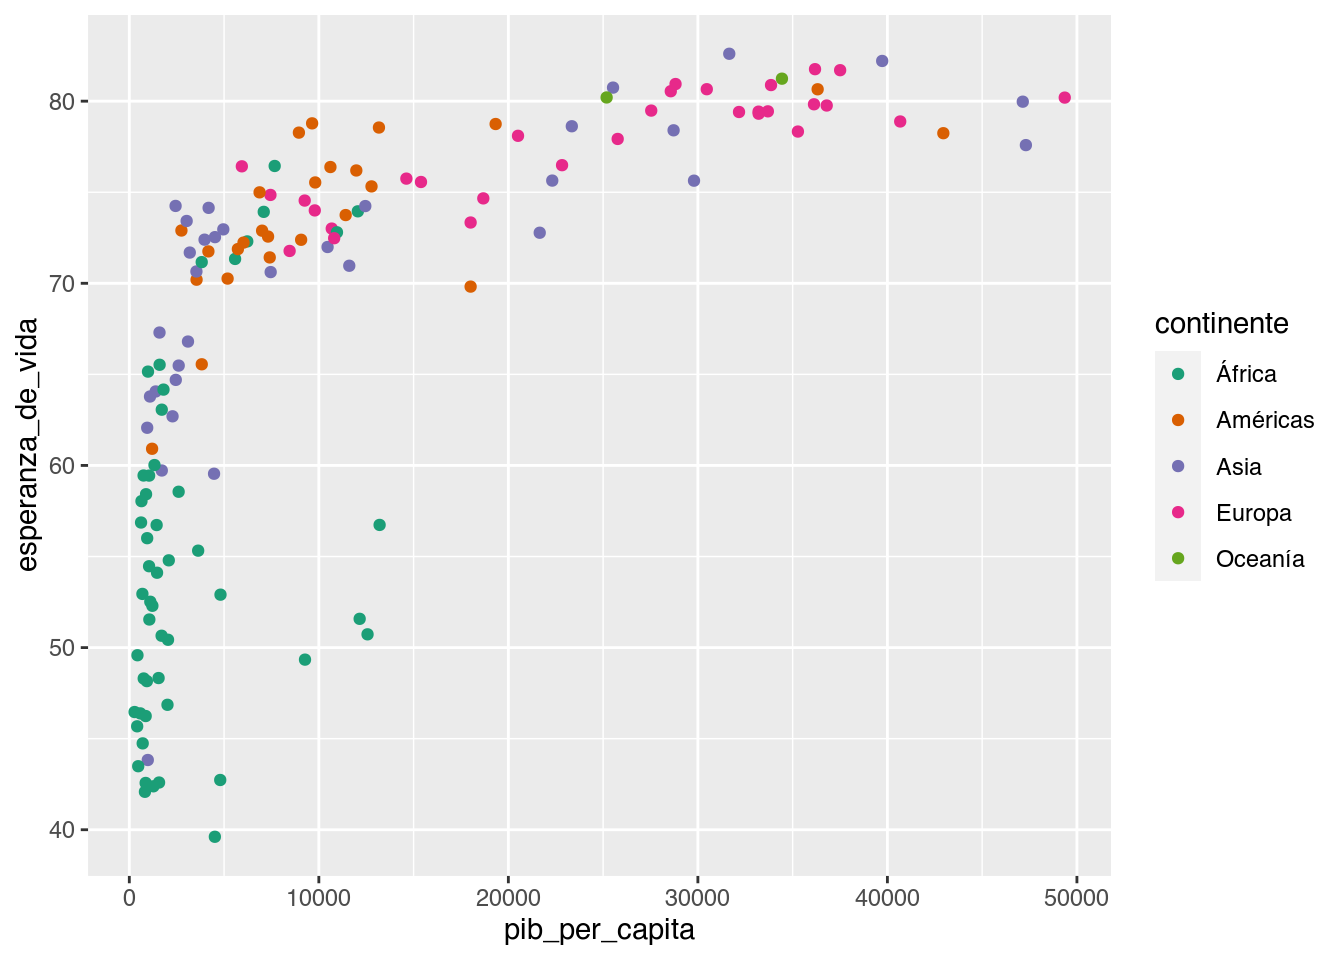
\includegraphics[width=1\linewidth]{DT6_files/figure-latex/unnamed-chunk-99-1} \end{center}

Nuestro gráfico va quedando mejor y podemos aprovechar la capacidad de \{ggplot2\} de \emph{mapear} variables a los elementos del gráfico y mostrar la población de cada país.

\textbf{Desafío}

A modo de prueba, cambia la paleta de colores actual por la de Viridis.
Para eso tenés que usar \texttt{scale\_color\_viridis\_d()}.
La ``d'' del final viene de \emph{discrete} y se usa para variables discretas o categorías, mientas que si los datos son continuos, se usa ``c''.

\begin{Shaded}
\begin{Highlighting}[]
\NormalTok{paises }\SpecialCharTok{\%\textgreater{}\%} 
  \FunctionTok{filter}\NormalTok{(anio }\SpecialCharTok{==} \DecValTok{2007}\NormalTok{) }\SpecialCharTok{\%\textgreater{}\%} 
  \FunctionTok{ggplot}\NormalTok{(}\FunctionTok{aes}\NormalTok{(pib\_per\_capita, esperanza\_de\_vida)) }\SpecialCharTok{+}
  \FunctionTok{geom\_point}\NormalTok{(}\FunctionTok{aes}\NormalTok{(}\AttributeTok{color =}\NormalTok{ continente, }\AttributeTok{size =}\NormalTok{ poblacion)) }\SpecialCharTok{+}
  \FunctionTok{scale\_color\_brewer}\NormalTok{(}\AttributeTok{type =} \StringTok{"qual"}\NormalTok{, }\AttributeTok{palette =} \StringTok{"Dark2"}\NormalTok{)}
\end{Highlighting}
\end{Shaded}

\begin{center}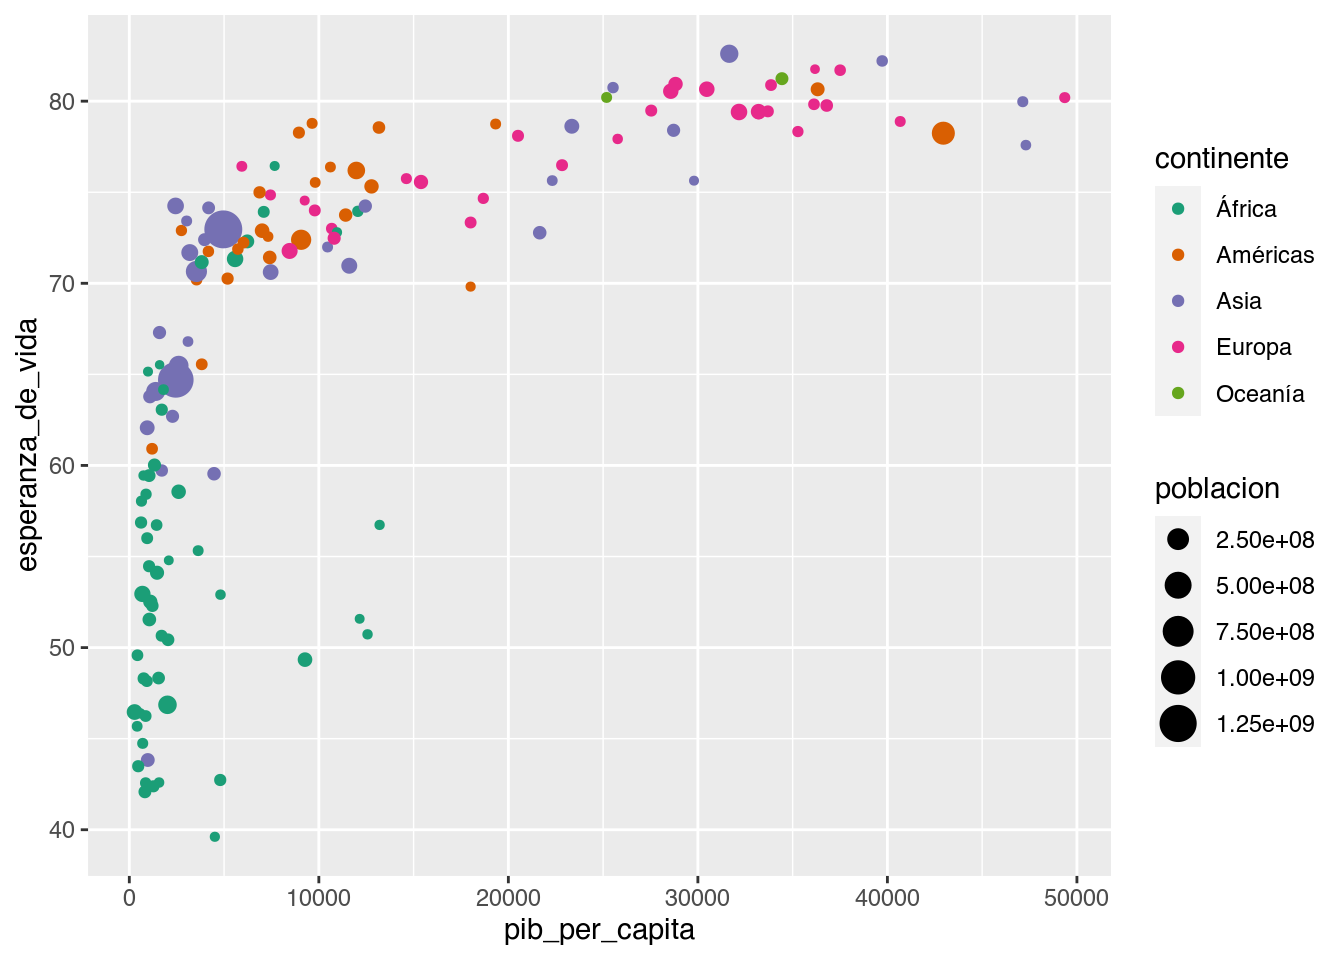
\includegraphics[width=1\linewidth]{DT6_files/figure-latex/unnamed-chunk-100-1} \end{center}

Esto nos da más información, pero al mismo tiempo vemos que los puntos se superponen.
Vamos a arreglar eso agregando transparencia y de paso modificar el tamaño de los puntos con la escala correspondiente \texttt{scale\_size()} y sacar la legenda con \texttt{guide\ =\ NULL}.

\begin{Shaded}
\begin{Highlighting}[]
\NormalTok{paises }\SpecialCharTok{\%\textgreater{}\%} 
  \FunctionTok{filter}\NormalTok{(anio }\SpecialCharTok{==} \DecValTok{2007}\NormalTok{) }\SpecialCharTok{\%\textgreater{}\%} 
  \FunctionTok{ggplot}\NormalTok{(}\FunctionTok{aes}\NormalTok{(pib\_per\_capita, esperanza\_de\_vida)) }\SpecialCharTok{+}
  \FunctionTok{geom\_point}\NormalTok{(}\FunctionTok{aes}\NormalTok{(}\AttributeTok{color =}\NormalTok{ continente, }\AttributeTok{size =}\NormalTok{ poblacion), }\AttributeTok{alpha =} \FloatTok{0.5}\NormalTok{) }\SpecialCharTok{+}
  \FunctionTok{scale\_color\_brewer}\NormalTok{(}\AttributeTok{type =} \StringTok{"qual"}\NormalTok{, }\AttributeTok{palette =} \StringTok{"Dark2"}\NormalTok{) }\SpecialCharTok{+}
  \FunctionTok{scale\_size\_area}\NormalTok{(}\AttributeTok{max\_size =} \DecValTok{15}\NormalTok{, }\AttributeTok{guide =} \ConstantTok{NULL}\NormalTok{)}
\end{Highlighting}
\end{Shaded}

\begin{center}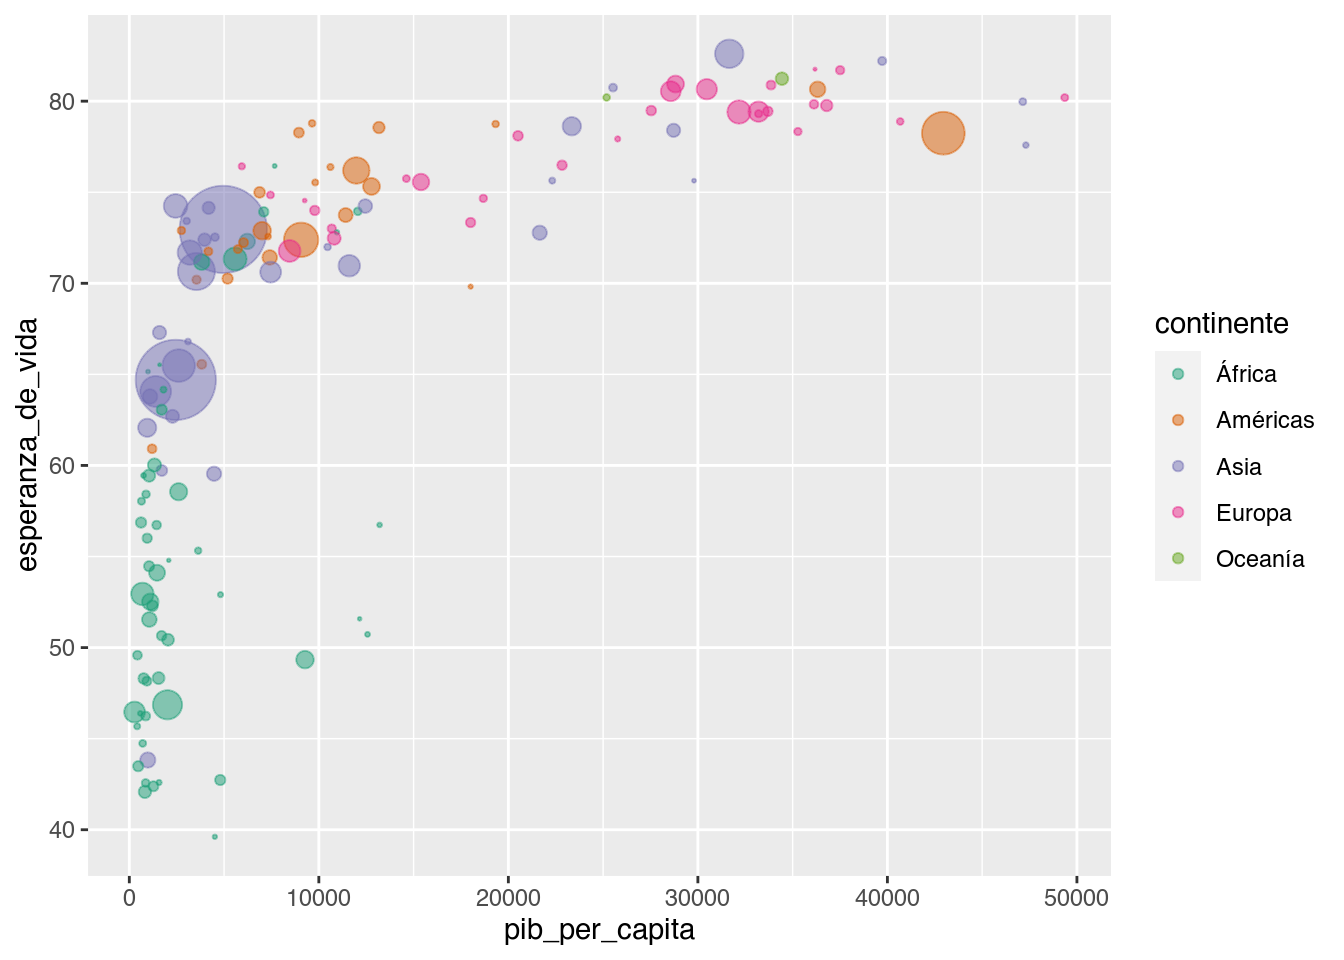
\includegraphics[width=1\linewidth]{DT6_files/figure-latex/unnamed-chunk-101-1} \end{center}

\hypertarget{escalas-de-ejes}{%
\subsection{Escalas de ejes}\label{escalas-de-ejes}}

Tal vez notaste que el comportamiento entre la esperanza de vida y el PBI no es lineal, de hecho el PBI varía mucho mientras que la esperanza de vida va apenas entre 40 y 80 y algo.
Eso puede esta indicando que el PBI tiene un comportamiento \emph{logarítmico} y si bien podríamos transformar los datos antes de hacer el gráfico, también podemos elegir una escala logarítmica para el eje del gráfico correspondiente.

\begin{Shaded}
\begin{Highlighting}[]
\NormalTok{paises }\SpecialCharTok{\%\textgreater{}\%} 
  \FunctionTok{filter}\NormalTok{(anio }\SpecialCharTok{==} \DecValTok{2007}\NormalTok{) }\SpecialCharTok{\%\textgreater{}\%} 
  \FunctionTok{ggplot}\NormalTok{(}\FunctionTok{aes}\NormalTok{(pib\_per\_capita, esperanza\_de\_vida)) }\SpecialCharTok{+}
  \FunctionTok{geom\_point}\NormalTok{(}\FunctionTok{aes}\NormalTok{(}\AttributeTok{color =}\NormalTok{ continente, }\AttributeTok{size =}\NormalTok{ poblacion), }\AttributeTok{alpha =} \FloatTok{0.5}\NormalTok{) }\SpecialCharTok{+}
  \FunctionTok{scale\_color\_brewer}\NormalTok{(}\AttributeTok{type =} \StringTok{"qual"}\NormalTok{, }\AttributeTok{palette =} \StringTok{"Dark2"}\NormalTok{) }\SpecialCharTok{+}
  \FunctionTok{scale\_size\_area}\NormalTok{(}\AttributeTok{max\_size =} \DecValTok{15}\NormalTok{, }\AttributeTok{guide =} \ConstantTok{NULL}\NormalTok{) }\SpecialCharTok{+}
  \FunctionTok{scale\_x\_log10}\NormalTok{()}
\end{Highlighting}
\end{Shaded}

\begin{center}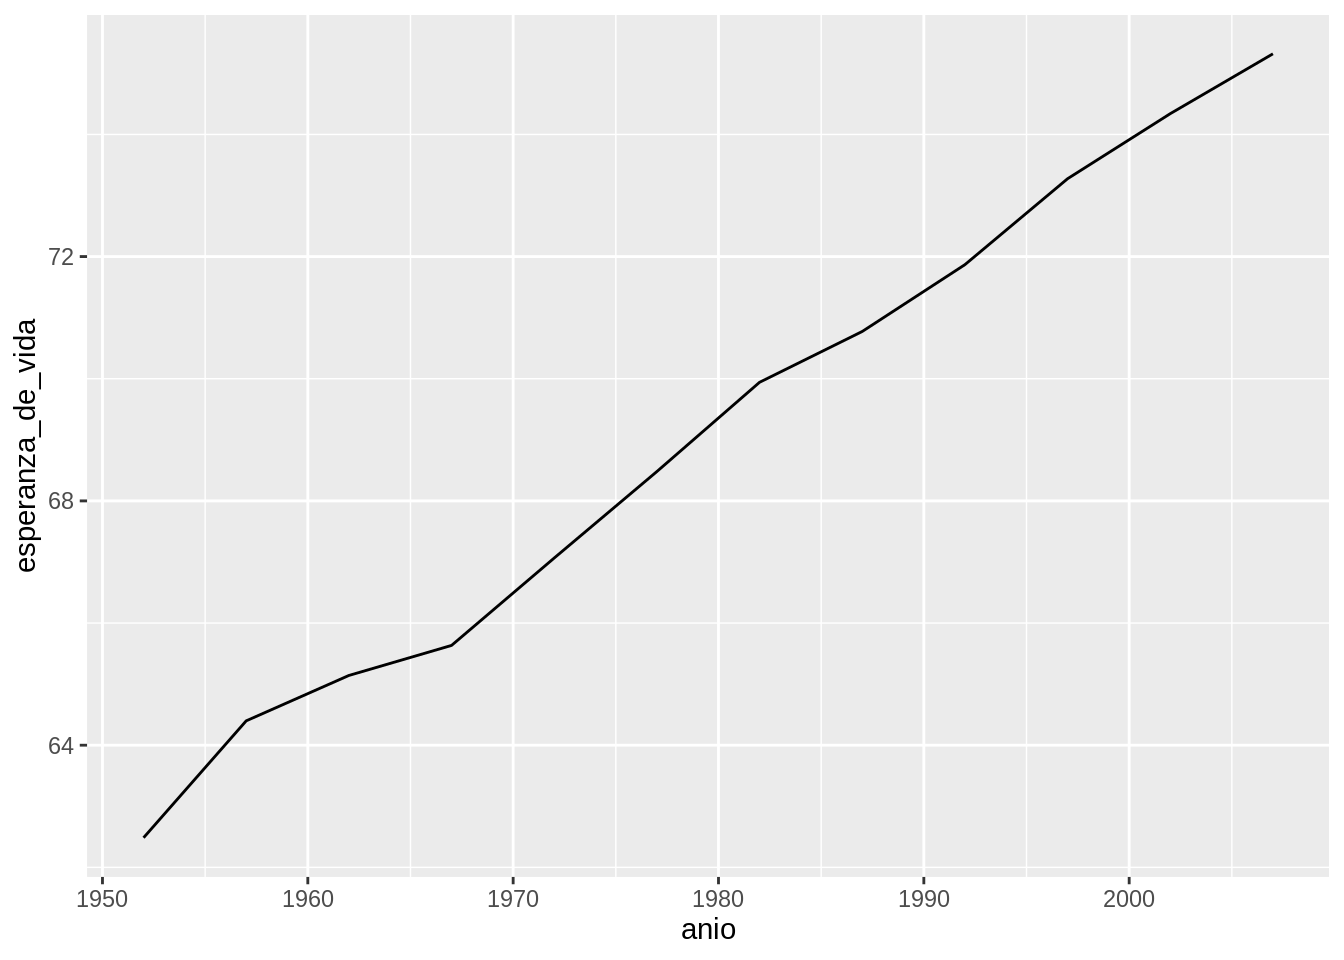
\includegraphics[width=1\linewidth]{DT6_files/figure-latex/unnamed-chunk-102-1} \end{center}

En este caso las escalas que modifican los ejes justamente comienzan con \texttt{scala\_x\_} o \texttt{scale\_y\_} según sea el caso.
Y por supuesto hay una variedad importante de escalas con muchas opciones.

\hypertarget{elementos-de-texto}{%
\section{Elementos de texto}\label{elementos-de-texto}}

Ya sumamos 3 escalas, pero el gráfico ya se ve muy bien.
¿Cómo hacemos si queremos identificar países individuales?
Por ahora es difícil, pero podríamos agregar etiquetas de texto con el nombre de cada país al lado de cada punto usando \texttt{geom\_text()}, y en este caso la apariencia está dada por \texttt{label} o etiqueta:

\begin{Shaded}
\begin{Highlighting}[]
\NormalTok{paises }\SpecialCharTok{\%\textgreater{}\%} 
  \FunctionTok{filter}\NormalTok{(anio }\SpecialCharTok{==} \DecValTok{2007}\NormalTok{) }\SpecialCharTok{\%\textgreater{}\%} 
  \FunctionTok{ggplot}\NormalTok{(}\FunctionTok{aes}\NormalTok{(pib\_per\_capita, esperanza\_de\_vida)) }\SpecialCharTok{+}
  \FunctionTok{geom\_point}\NormalTok{(}\FunctionTok{aes}\NormalTok{(}\AttributeTok{color =}\NormalTok{ continente, }\AttributeTok{size =}\NormalTok{ poblacion), }\AttributeTok{alpha =} \FloatTok{0.5}\NormalTok{) }\SpecialCharTok{+}
  \FunctionTok{scale\_color\_brewer}\NormalTok{(}\AttributeTok{type =} \StringTok{"qual"}\NormalTok{, }\AttributeTok{palette =} \StringTok{"Dark2"}\NormalTok{) }\SpecialCharTok{+}
  \FunctionTok{scale\_size\_area}\NormalTok{(}\AttributeTok{max\_size =} \DecValTok{15}\NormalTok{, }\AttributeTok{guide =} \ConstantTok{NULL}\NormalTok{) }\SpecialCharTok{+}
  \FunctionTok{scale\_x\_log10}\NormalTok{() }\SpecialCharTok{+}
  \FunctionTok{geom\_text}\NormalTok{(}\FunctionTok{aes}\NormalTok{(}\AttributeTok{label =}\NormalTok{ pais)) }
\end{Highlighting}
\end{Shaded}

\begin{center}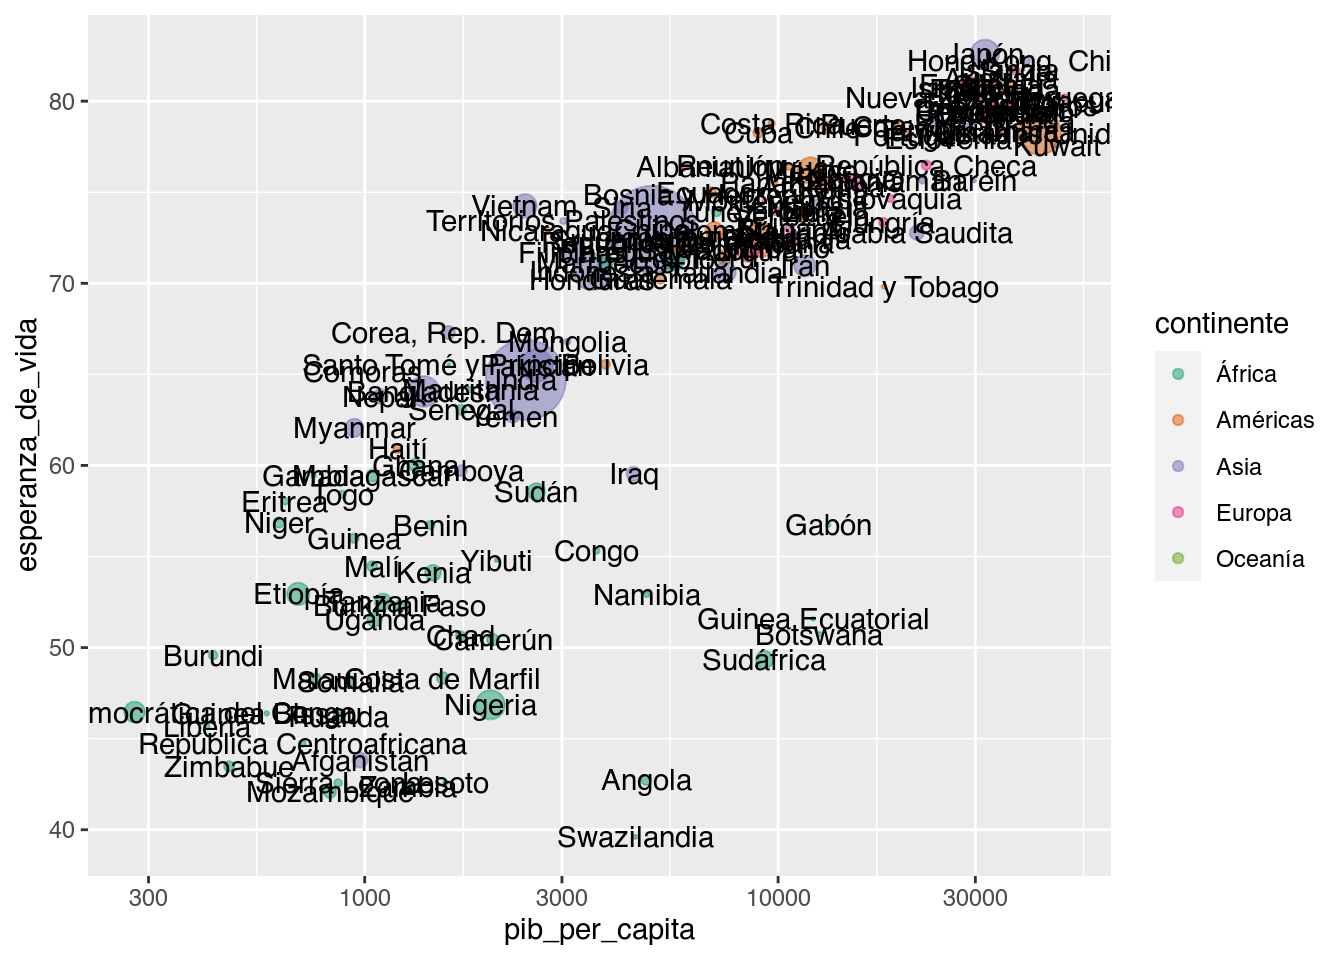
\includegraphics[width=1\linewidth]{DT6_files/figure-latex/unnamed-chunk-103-1} \end{center}

Pero nos olvidamos que tenemos casi 200 países, es razonable agregarle etiquetas a todos.
Pero podríamos querer resaltar algunos, tal vez los de un continente en particular o los que cumplen con la condición de tener las mayores poblaciones del mundo.
Para eso vamos a generarnos una nueva tabla con los países que queremos resaltar y de paso usarla dentro de \texttt{geom\_text()}.

\begin{Shaded}
\begin{Highlighting}[]
\NormalTok{mucha\_poblacion }\OtherTok{\textless{}{-}}\NormalTok{ paises }\SpecialCharTok{\%\textgreater{}\%} 
  \FunctionTok{filter}\NormalTok{(anio }\SpecialCharTok{==} \DecValTok{2007}\NormalTok{) }\SpecialCharTok{\%\textgreater{}\%} 
  \FunctionTok{filter}\NormalTok{(poblacion }\SpecialCharTok{\textgreater{}} \DecValTok{1000000000}\NormalTok{) }\CommentTok{\# Países con más de un billón de habitantes!}

\NormalTok{paises }\SpecialCharTok{\%\textgreater{}\%} 
  \FunctionTok{filter}\NormalTok{(anio }\SpecialCharTok{==} \DecValTok{2007}\NormalTok{) }\SpecialCharTok{\%\textgreater{}\%} 
  \FunctionTok{ggplot}\NormalTok{(}\FunctionTok{aes}\NormalTok{(pib\_per\_capita, esperanza\_de\_vida)) }\SpecialCharTok{+}
  \FunctionTok{geom\_point}\NormalTok{(}\FunctionTok{aes}\NormalTok{(}\AttributeTok{color =}\NormalTok{ continente, }\AttributeTok{size =}\NormalTok{ poblacion), }\AttributeTok{alpha =} \FloatTok{0.5}\NormalTok{) }\SpecialCharTok{+}
  \FunctionTok{scale\_color\_brewer}\NormalTok{(}\AttributeTok{type =} \StringTok{"qual"}\NormalTok{, }\AttributeTok{palette =} \StringTok{"Dark2"}\NormalTok{) }\SpecialCharTok{+}
  \FunctionTok{scale\_size\_area}\NormalTok{(}\AttributeTok{max\_size =} \DecValTok{15}\NormalTok{, }\AttributeTok{guide =} \ConstantTok{NULL}\NormalTok{) }\SpecialCharTok{+}
  \FunctionTok{scale\_x\_log10}\NormalTok{() }\SpecialCharTok{+}
  \FunctionTok{geom\_text}\NormalTok{(}\FunctionTok{aes}\NormalTok{(}\AttributeTok{label =}\NormalTok{ pais), }
            \AttributeTok{data =}\NormalTok{ mucha\_poblacion)  }\CommentTok{\# Esta capa usa la tabla mucha\_población!}
\end{Highlighting}
\end{Shaded}

\begin{center}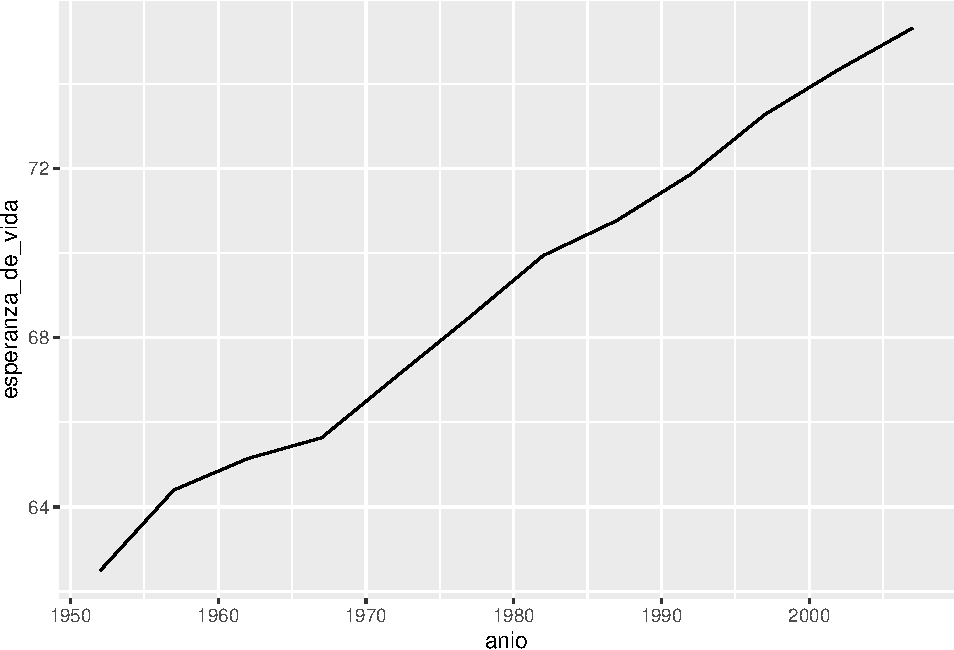
\includegraphics[width=1\linewidth]{DT6_files/figure-latex/unnamed-chunk-104-1} \end{center}

Del código anterior surge algo muy importante: es posible generar capas en un gráfico usando una data.frame \emph{distinto} al que usamos para graficar las capas anteriores.
Esto es útil principalmente para definir etiquetas o resaltar determinadas observaciones.

Y el truco está en que ambos data.frames tienen las variables \texttt{pib\_per\_capita} y \texttt{esperanza\_de\_vida} y entonces \{ggplot2\} puede identificar en que parte del gráfico (en que valores de x y en que valores de y) colocar cada elemento.

Veamos ahora una (de varias) maneras agregar o modificar elementos de texto en el gráfico.
Vamos a usar una nueva función (y una nueva capa!), \texttt{labs()}:

\begin{Shaded}
\begin{Highlighting}[]
\NormalTok{paises }\SpecialCharTok{\%\textgreater{}\%} 
  \FunctionTok{filter}\NormalTok{(anio }\SpecialCharTok{==} \DecValTok{2007}\NormalTok{) }\SpecialCharTok{\%\textgreater{}\%} 
  \FunctionTok{ggplot}\NormalTok{(}\FunctionTok{aes}\NormalTok{(pib\_per\_capita, esperanza\_de\_vida)) }\SpecialCharTok{+}
  \FunctionTok{geom\_point}\NormalTok{(}\FunctionTok{aes}\NormalTok{(}\AttributeTok{color =}\NormalTok{ continente, }\AttributeTok{size =}\NormalTok{ poblacion), }\AttributeTok{alpha =} \FloatTok{0.5}\NormalTok{) }\SpecialCharTok{+}
  \FunctionTok{scale\_color\_brewer}\NormalTok{(}\AttributeTok{type =} \StringTok{"qual"}\NormalTok{, }\AttributeTok{palette =} \StringTok{"Dark2"}\NormalTok{) }\SpecialCharTok{+}
  \FunctionTok{scale\_size\_area}\NormalTok{(}\AttributeTok{max\_size =} \DecValTok{15}\NormalTok{, }\AttributeTok{guide =} \ConstantTok{NULL}\NormalTok{) }\SpecialCharTok{+}
  \FunctionTok{scale\_x\_log10}\NormalTok{() }\SpecialCharTok{+}
  \FunctionTok{geom\_text}\NormalTok{(}\FunctionTok{aes}\NormalTok{(}\AttributeTok{label =}\NormalTok{ pais), }\AttributeTok{data =}\NormalTok{ mucha\_poblacion) }\SpecialCharTok{+}
  \FunctionTok{labs}\NormalTok{(}\AttributeTok{title =} \StringTok{"Paises del mundo"}\NormalTok{,}
       \AttributeTok{subtitle =} \StringTok{"Año 2007"}\NormalTok{,}
       \AttributeTok{caption =} \StringTok{"El tamaño de cada circulo representa la población."}\NormalTok{,}
       \AttributeTok{x =} \StringTok{"PBI per capita"}\NormalTok{,}
       \AttributeTok{y =} \StringTok{"Esperanza de vida"}\NormalTok{,}
       \AttributeTok{color =} \StringTok{""}\NormalTok{)}
\end{Highlighting}
\end{Shaded}

\begin{center}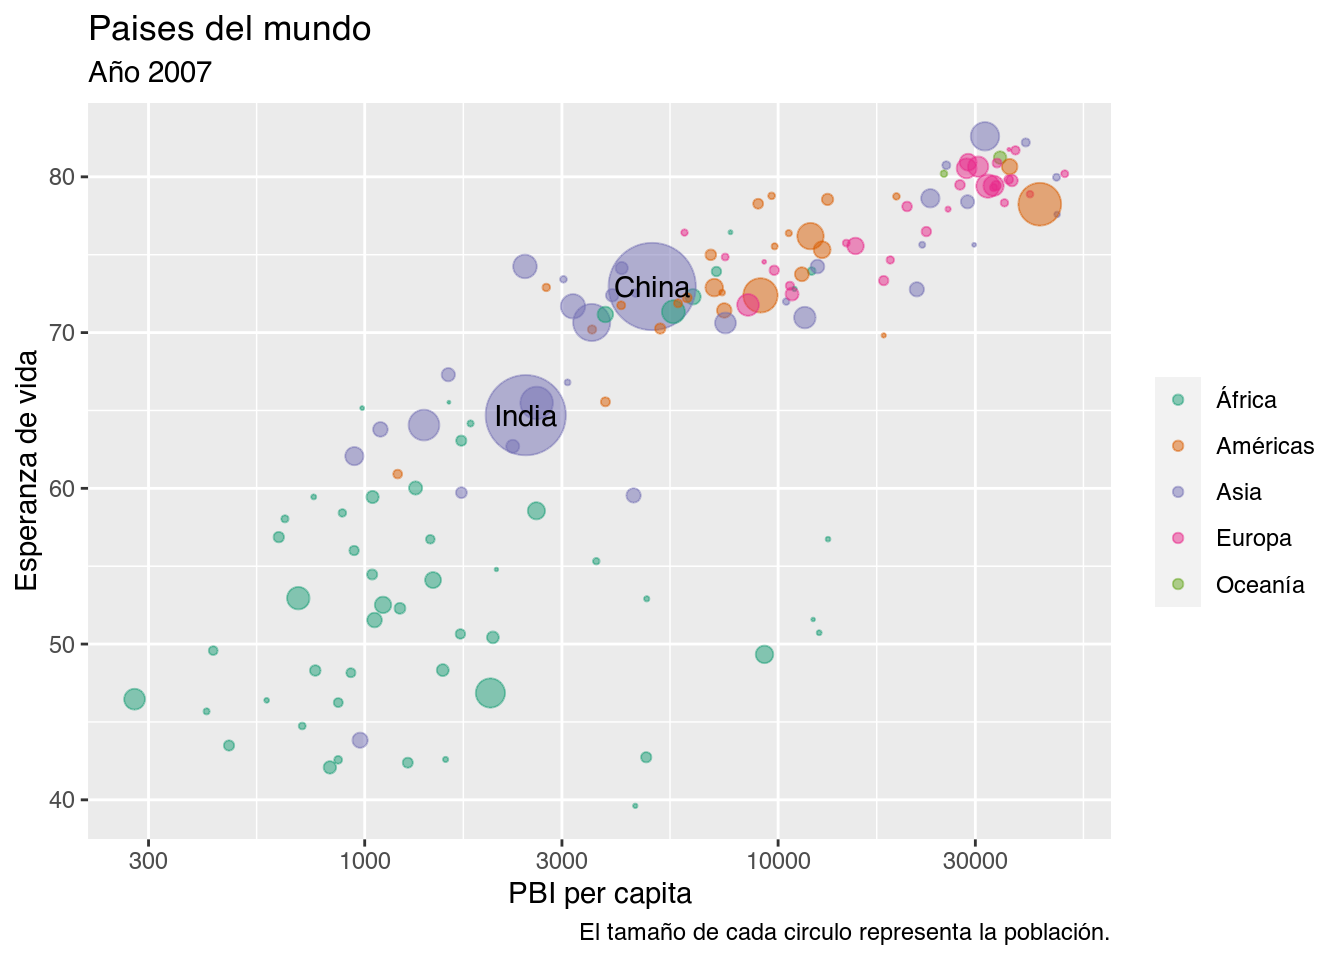
\includegraphics[width=1\linewidth]{DT6_files/figure-latex/unnamed-chunk-105-1} \end{center}

Agregamos un título, un subtítulo, el epígrafe de la figura (\emph{caption}) para las aclaraciones y cambiamos el nombre de los ejes para que se vean mejor.
Pero ademas eliminamos el nombre de la leyenda porque era un poco redundante.

\hypertarget{temas}{%
\section{Temas}\label{temas}}

Nos queda una última cosa por hacer, cambiar la apariencia global del gráfico.
\{ggplot2\} tiene muchos \emph{temas} disponibles y para todos los gustos.
Pero además hay otros paquetes que extienden las posibilidades, por ejemplo \href{https://github.com/jrnold/ggthemes}{\{ggthemes\}}.

Por defecto \{ggplot2\} usa \texttt{theme\_grey()}, probemos \texttt{theme\_light()}:

\begin{Shaded}
\begin{Highlighting}[]
\NormalTok{paises }\SpecialCharTok{\%\textgreater{}\%} 
  \FunctionTok{filter}\NormalTok{(anio }\SpecialCharTok{==} \DecValTok{2007}\NormalTok{) }\SpecialCharTok{\%\textgreater{}\%} 
  \FunctionTok{ggplot}\NormalTok{(}\FunctionTok{aes}\NormalTok{(pib\_per\_capita, esperanza\_de\_vida)) }\SpecialCharTok{+}
  \FunctionTok{geom\_point}\NormalTok{(}\FunctionTok{aes}\NormalTok{(}\AttributeTok{color =}\NormalTok{ continente, }\AttributeTok{size =}\NormalTok{ poblacion), }\AttributeTok{alpha =} \FloatTok{0.5}\NormalTok{) }\SpecialCharTok{+}
  \FunctionTok{scale\_color\_brewer}\NormalTok{(}\AttributeTok{type =} \StringTok{"qual"}\NormalTok{, }\AttributeTok{palette =} \StringTok{"Dark2"}\NormalTok{) }\SpecialCharTok{+}
  \FunctionTok{scale\_size\_area}\NormalTok{(}\AttributeTok{max\_size =} \DecValTok{15}\NormalTok{, }\AttributeTok{guide =} \ConstantTok{NULL}\NormalTok{) }\SpecialCharTok{+}
  \FunctionTok{scale\_x\_log10}\NormalTok{() }\SpecialCharTok{+}
  \FunctionTok{geom\_text}\NormalTok{(}\FunctionTok{aes}\NormalTok{(}\AttributeTok{label =}\NormalTok{ pais), }\AttributeTok{data =}\NormalTok{ mucha\_poblacion) }\SpecialCharTok{+}
  \FunctionTok{labs}\NormalTok{(}\AttributeTok{title =} \StringTok{"Paises del mundo"}\NormalTok{,}
       \AttributeTok{subtitle =} \StringTok{"Año 2007"}\NormalTok{,}
       \AttributeTok{caption =} \StringTok{"El tamaño de cada circulo representa la población."}\NormalTok{,}
       \AttributeTok{x =} \StringTok{"PBI per capita"}\NormalTok{,}
       \AttributeTok{y =} \StringTok{"Esperanza de vida"}\NormalTok{,}
       \AttributeTok{color =} \StringTok{""}\NormalTok{) }\SpecialCharTok{+}
  \FunctionTok{theme\_light}\NormalTok{()}
\end{Highlighting}
\end{Shaded}

\begin{center}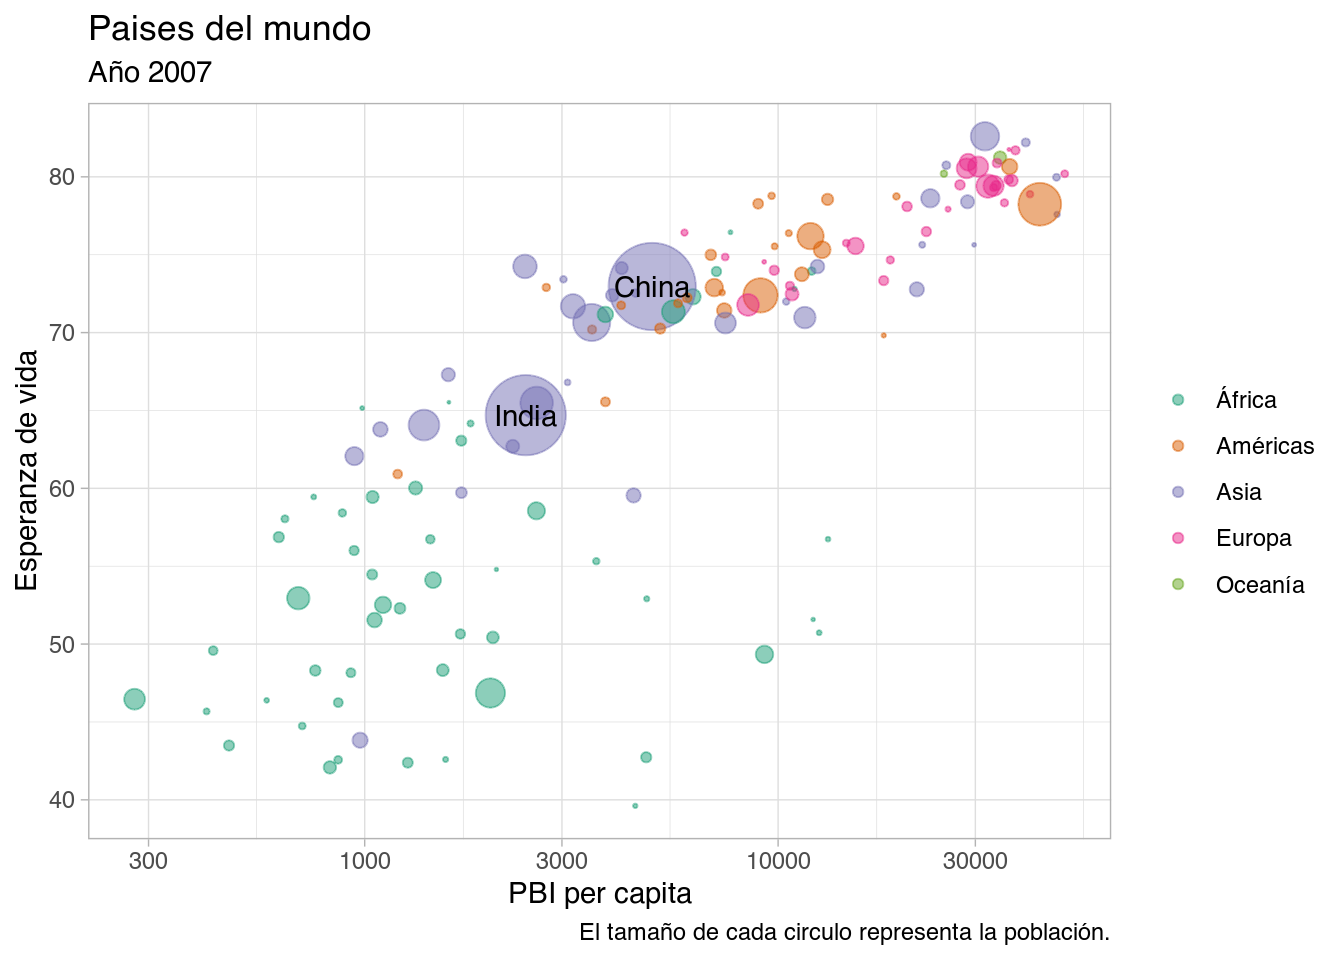
\includegraphics[width=1\linewidth]{DT6_files/figure-latex/unnamed-chunk-106-1} \end{center}

Ahora es tu turno.
Elegí un \href{https://es.r4ds.hadley.nz/images/visualization-themes.png}{tema que te guste} y probalo.
Además, si se te ocurre algún título mejor modificalo!

Junto con las funciones \texttt{theme\_...()}, hay una función llamada \texttt{theme()} que permite cambiar la apariencia de cualquier elemento del gráfico.
Tiene casi infinitas opciones y si algún momento te desvelas intentando cambiar esa línea o ese borde, seguro que \texttt{theme()} tiene alguna opción para hacer eso.

Anterior Hoja de ruta

\hypertarget{desafuxedos-de-pruxe1ctica}{%
\chapter{Desafíos de práctica}\label{desafuxedos-de-pruxe1ctica}}

En esta sección te proponemos desafíos y ejercicios para prácticar o revisar lo que vimos en los distintos capítulos. Cada una de las subsección estará asociada a un conjunto de capítulos y buscan relacionar los distintos temas y herramientas.

\hypertarget{desafuxedo-1}{%
\section{Desafío 1}\label{desafuxedo-1}}

\textbf{Capítulos asociados:} Instalación de R y Rstudio, Uso de proyectos, Reportes con RMarkdown y lectura de datos.

\begin{enumerate}
\def\labelenumi{\arabic{enumi}.}
\item
  Seguí las instrucciones que encontrarás en el \href{}{Anexo I} para instalar R y Rstudio. Tené en cuenta que la instalación en computadoras con Windows requieren algunos pasos extra.
\item
  Abrí RStudio y creá tu primer proyecto. Este proyecto te acompañará a lo largo de todos los desafíos y ejercicios de este libro, por lo que va a necesitar un nombre fácil de recordar. Podés revisar las instrucciones \href{}{acá}.
\item
  Ahora es momento de instalar algunos paquetes para poder usar luego. Por ahora instalemos readr, remotes y datos.
\end{enumerate}

\begin{Shaded}
\begin{Highlighting}[]
\FunctionTok{install.packages}\NormalTok{(}\StringTok{"readr"}\NormalTok{)}
\FunctionTok{install.packages}\NormalTok{(}\StringTok{"remotes"}\NormalTok{)}
\NormalTok{remotes}\SpecialCharTok{::}\FunctionTok{install\_github}\NormalTok{(}\StringTok{"ciencia\_datos/datos"}\NormalTok{)}
\end{Highlighting}
\end{Shaded}

La tercera linea, si bien distinta a las anteriores, también instala un paqute. La diferencia es que instala el paquete desde un repositorio de GitHub donde suelen estar los paquetes en desarrollo.

\begin{enumerate}
\def\labelenumi{\arabic{enumi}.}
\setcounter{enumi}{3}
\item
  Creá un nuevo archivo R Markdown que se llame ``01-lectura.Rmd'' desde File -\textgreater{} New File -\textgreater{} R Markdown. Si bien el archivo puede tener cualquer nombre, siempre que sea informativo, te proponemos nombrarlos como número-nombre para poder ordenarlos y que te resulte más fácil encontrarlo dentro del proyecto. Borrá la plantilla y guardá el archivo. Para guardar File -\textgreater{} Save o click en en el disquette 💾. Es posible que necesites darle permiso a RStudio para que instale nuevos paquetes asociados a R Markdown.
\item
  Aprovechemos el archivo recien creado para leer datos. Te proponemos que revises el capítulo de {[}lectura de datos{]} y sigas las instrucciones para leer los datos.
\item
  ¡Listo! En la próxima sección practicaremos con esos y otros datos.
\end{enumerate}

\hypertarget{desafuxedo-2}{%
\section{Desafío 2}\label{desafuxedo-2}}

\textbf{Capítulos asociados:} Manipulación de datos con dplyr y la primera parte de gráficos con ggplot2

\hypertarget{desafuxedo-3}{%
\section{Desafío 3}\label{desafuxedo-3}}

\textbf{Capítulos asociados:} Más gráficos con ggplot2 y manupulación de datos con dplyr y tidyr.

\hypertarget{desafuxedo-4}{%
\section{Desafío 4}\label{desafuxedo-4}}

\textbf{Capítulos asociados:} Tablas, gráficos e informes para publicar.

\hypertarget{appendix-apuxe9ndice}{%
\appendix}


\hypertarget{instalando-r-y-rstudio}{%
\chapter{Instalando R y RStudio}\label{instalando-r-y-rstudio}}

\hypertarget{windows}{%
\section{Windows}\label{windows}}

Entrá a \url{https://cran.r-project.org/bin/windows/base/} y bajate el instalador haciendo click en el link grandote que dice ``Download R 4.0.5 for Windows''. Una vez que se bajó, hacé doble click en el archivo y seguí las instrucciones del instalador.

Una vez que se termine de instalar, te va a aparecer un ícono como este en el escritorio o en los programas instalados R Programming Language icon PNG and SVG Vector Free Download

Al ejecturalo, les tiene que aparecer algo como esto:

R for Windows Descargar (2021 Última versión) para Windows 10, 8, 7

Para instalar algunos paquetes de R vas a necesitar instalar un adicional llamado rtools40. Entrá a \url{https://cran.r-project.org/bin/windows/Rtools/} y descargate el instalador en donde dice ``On Windows 64-bit: rtools40-x86\_64.exe (recommended: includes both i386 and x64 compilers)''

Finalmente abrí RStudio y en la consola poné esto y apretá enter:

writeLines(`PATH=``\({RTOOLS40_HOME}\\usr\\bin;\)\{PATH\}''\,', con = ``\textasciitilde/.Renviron'')

Finalmente, para chequear que todo esté bien, cerrá RStudio, volvé a abrirlo y escribí esto en la consolsa y apretá enter:

Sys.which(``make'')
Debería salir algo como esto:

``C:\textbackslash rtools40\textbackslash usr\textbackslash bin\textbackslash make.exe''

\end{document}
